% Options for packages loaded elsewhere
\PassOptionsToPackage{unicode}{hyperref}
\PassOptionsToPackage{hyphens}{url}
\PassOptionsToPackage{dvipsnames,svgnames,x11names}{xcolor}
%
\documentclass[
  12pt,
  a4paper,
]{scrreprt}

\usepackage{amsmath,amssymb}
\usepackage{iftex}
\ifPDFTeX
  \usepackage[T1]{fontenc}
  \usepackage[utf8]{inputenc}
  \usepackage{textcomp} % provide euro and other symbols
\else % if luatex or xetex
  \usepackage{unicode-math}
  \defaultfontfeatures{Scale=MatchLowercase}
  \defaultfontfeatures[\rmfamily]{Ligatures=TeX,Scale=1}
\fi
\usepackage{lmodern}
\ifPDFTeX\else  
    % xetex/luatex font selection
\fi
% Use upquote if available, for straight quotes in verbatim environments
\IfFileExists{upquote.sty}{\usepackage{upquote}}{}
\IfFileExists{microtype.sty}{% use microtype if available
  \usepackage[]{microtype}
  \UseMicrotypeSet[protrusion]{basicmath} % disable protrusion for tt fonts
}{}
\usepackage{xcolor}
\usepackage[left=3cm,,right=2cm,,top=3cm,,bottom=2cm]{geometry}
\setlength{\emergencystretch}{3em} % prevent overfull lines
\setcounter{secnumdepth}{5}

\usepackage{color}
\usepackage{fancyvrb}
\newcommand{\VerbBar}{|}
\newcommand{\VERB}{\Verb[commandchars=\\\{\}]}
\DefineVerbatimEnvironment{Highlighting}{Verbatim}{commandchars=\\\{\}}
% Add ',fontsize=\small' for more characters per line
\newenvironment{Shaded}{}{}
\newcommand{\AlertTok}[1]{\textcolor[rgb]{1.00,0.33,0.33}{\textbf{#1}}}
\newcommand{\AnnotationTok}[1]{\textcolor[rgb]{0.42,0.45,0.49}{#1}}
\newcommand{\AttributeTok}[1]{\textcolor[rgb]{0.84,0.23,0.29}{#1}}
\newcommand{\BaseNTok}[1]{\textcolor[rgb]{0.00,0.36,0.77}{#1}}
\newcommand{\BuiltInTok}[1]{\textcolor[rgb]{0.84,0.23,0.29}{#1}}
\newcommand{\CharTok}[1]{\textcolor[rgb]{0.01,0.18,0.38}{#1}}
\newcommand{\CommentTok}[1]{\textcolor[rgb]{0.42,0.45,0.49}{#1}}
\newcommand{\CommentVarTok}[1]{\textcolor[rgb]{0.42,0.45,0.49}{#1}}
\newcommand{\ConstantTok}[1]{\textcolor[rgb]{0.00,0.36,0.77}{#1}}
\newcommand{\ControlFlowTok}[1]{\textcolor[rgb]{0.84,0.23,0.29}{#1}}
\newcommand{\DataTypeTok}[1]{\textcolor[rgb]{0.84,0.23,0.29}{#1}}
\newcommand{\DecValTok}[1]{\textcolor[rgb]{0.00,0.36,0.77}{#1}}
\newcommand{\DocumentationTok}[1]{\textcolor[rgb]{0.42,0.45,0.49}{#1}}
\newcommand{\ErrorTok}[1]{\textcolor[rgb]{1.00,0.33,0.33}{\underline{#1}}}
\newcommand{\ExtensionTok}[1]{\textcolor[rgb]{0.84,0.23,0.29}{\textbf{#1}}}
\newcommand{\FloatTok}[1]{\textcolor[rgb]{0.00,0.36,0.77}{#1}}
\newcommand{\FunctionTok}[1]{\textcolor[rgb]{0.44,0.26,0.76}{#1}}
\newcommand{\ImportTok}[1]{\textcolor[rgb]{0.01,0.18,0.38}{#1}}
\newcommand{\InformationTok}[1]{\textcolor[rgb]{0.42,0.45,0.49}{#1}}
\newcommand{\KeywordTok}[1]{\textcolor[rgb]{0.84,0.23,0.29}{#1}}
\newcommand{\NormalTok}[1]{\textcolor[rgb]{0.14,0.16,0.18}{#1}}
\newcommand{\OperatorTok}[1]{\textcolor[rgb]{0.14,0.16,0.18}{#1}}
\newcommand{\OtherTok}[1]{\textcolor[rgb]{0.44,0.26,0.76}{#1}}
\newcommand{\PreprocessorTok}[1]{\textcolor[rgb]{0.84,0.23,0.29}{#1}}
\newcommand{\RegionMarkerTok}[1]{\textcolor[rgb]{0.42,0.45,0.49}{#1}}
\newcommand{\SpecialCharTok}[1]{\textcolor[rgb]{0.00,0.36,0.77}{#1}}
\newcommand{\SpecialStringTok}[1]{\textcolor[rgb]{0.01,0.18,0.38}{#1}}
\newcommand{\StringTok}[1]{\textcolor[rgb]{0.01,0.18,0.38}{#1}}
\newcommand{\VariableTok}[1]{\textcolor[rgb]{0.89,0.38,0.04}{#1}}
\newcommand{\VerbatimStringTok}[1]{\textcolor[rgb]{0.01,0.18,0.38}{#1}}
\newcommand{\WarningTok}[1]{\textcolor[rgb]{1.00,0.33,0.33}{#1}}

\providecommand{\tightlist}{%
  \setlength{\itemsep}{0pt}\setlength{\parskip}{0pt}}\usepackage{longtable,booktabs,array}
\usepackage{calc} % for calculating minipage widths
% Correct order of tables after \paragraph or \subparagraph
\usepackage{etoolbox}
\makeatletter
\patchcmd\longtable{\par}{\if@noskipsec\mbox{}\fi\par}{}{}
\makeatother
% Allow footnotes in longtable head/foot
\IfFileExists{footnotehyper.sty}{\usepackage{footnotehyper}}{\usepackage{footnote}}
\makesavenoteenv{longtable}
\usepackage{graphicx}
\makeatletter
\newsavebox\pandoc@box
\newcommand*\pandocbounded[1]{% scales image to fit in text height/width
  \sbox\pandoc@box{#1}%
  \Gscale@div\@tempa{\textheight}{\dimexpr\ht\pandoc@box+\dp\pandoc@box\relax}%
  \Gscale@div\@tempb{\linewidth}{\wd\pandoc@box}%
  \ifdim\@tempb\p@<\@tempa\p@\let\@tempa\@tempb\fi% select the smaller of both
  \ifdim\@tempa\p@<\p@\scalebox{\@tempa}{\usebox\pandoc@box}%
  \else\usebox{\pandoc@box}%
  \fi%
}
% Set default figure placement to htbp
\def\fps@figure{htbp}
\makeatother
% definitions for citeproc citations
\NewDocumentCommand\citeproctext{}{}
\NewDocumentCommand\citeproc{mm}{%
  \begingroup\def\citeproctext{#2}\cite{#1}\endgroup}
\makeatletter
 % allow citations to break across lines
 \let\@cite@ofmt\@firstofone
 % avoid brackets around text for \cite:
 \def\@biblabel#1{}
 \def\@cite#1#2{{#1\if@tempswa , #2\fi}}
\makeatother
\newlength{\cslhangindent}
\setlength{\cslhangindent}{1.5em}
\newlength{\csllabelwidth}
\setlength{\csllabelwidth}{3em}
\newenvironment{CSLReferences}[2] % #1 hanging-indent, #2 entry-spacing
 {\begin{list}{}{%
  \setlength{\itemindent}{0pt}
  \setlength{\leftmargin}{0pt}
  \setlength{\parsep}{0pt}
  % turn on hanging indent if param 1 is 1
  \ifodd #1
   \setlength{\leftmargin}{\cslhangindent}
   \setlength{\itemindent}{-1\cslhangindent}
  \fi
  % set entry spacing
  \setlength{\itemsep}{#2\baselineskip}}}
 {\end{list}}
\usepackage{calc}
\newcommand{\CSLBlock}[1]{\hfill\break\parbox[t]{\linewidth}{\strut\ignorespaces#1\strut}}
\newcommand{\CSLLeftMargin}[1]{\parbox[t]{\csllabelwidth}{\strut#1\strut}}
\newcommand{\CSLRightInline}[1]{\parbox[t]{\linewidth - \csllabelwidth}{\strut#1\strut}}
\newcommand{\CSLIndent}[1]{\hspace{\cslhangindent}#1}

\usepackage{pdfpages}
\usepackage{amsmath,amssymb}
\usepackage{dirtree}
\usepackage{amsmath}
\usepackage[explicit]{titlesec}
\usepackage{setspace}
\usepackage{caption}
\usepackage[hang,flushmargin]{footmisc}
\usepackage{etoolbox}
\usepackage[shortlabels]{enumitem}
\usepackage{booktabs}
\usepackage{ragged2e}
\usepackage{pdflscape}
\usepackage{fancyhdr}

\DeclareMathOperator{\E}{\mathbb{E}}
\newcommand{\blandscape}{\begin{landscape}}
\newcommand{\elandscape}{\end{landscape}}
\renewcommand{\footnotesize}{\scriptsize}
\renewcommand{\footnoterule}{\noindent\rule{5cm}{0.4pt}\vspace{0.2cm}}
\setlength{\footnotesep}{0.5em}

\setlength{\parskip}{0.0em}
\AtBeginEnvironment{quote}{\setstretch{1.0}}

\titleformat{\section}{\normalfont\large\bfseries}{}{0pt}{\thesection\quad#1}[]
\titleformat{\subsection}{\normalfont\normalsize\bfseries}{}{0pt}{\thesubsection\quad#1}[]
\titleformat{\subsubsection}{\normalfont\normalsize\itshape}{}{0pt}{#1}[]
\titleformat{\paragraph}[runin]{\normalfont\normalsize\bfseries}{}{0pt}{#1}[]
\titleformat{\subparagraph}[runin]{\normalfont\normalsize\itshape}{}{0pt}{#1}[]

\titlespacing*{\section}{0pt}{20pt}{10pt}
\titlespacing*{\subsection}{0pt}{15pt}{10pt}
\titlespacing*{\subsubsection}{0pt}{10pt}{10pt}
\titlespacing*{\paragraph}{0pt}{10pt}{10pt}
\titlespacing*{\subparagraph}{0pt}{10pt}{10pt}
\makeatletter
\@ifpackageloaded{float}{}{\usepackage{float}}
\floatstyle{plain}
\@ifundefined{c@chapter}{\newfloat{algo}{h}{loalgo}}{\newfloat{algo}{h}{loalgo}[chapter]}
\floatname{algo}{Algoritmo}
\newcommand*\listofalgos{\listof{algo}{List of Algoritmos}}
\makeatother
\makeatletter
\@ifpackageloaded{caption}{}{\usepackage{caption}}
\AtBeginDocument{%
\ifdefined\contentsname
  \renewcommand*\contentsname{Índice}
\else
  \newcommand\contentsname{Índice}
\fi
\ifdefined\listfigurename
  \renewcommand*\listfigurename{Lista de Figuras}
\else
  \newcommand\listfigurename{Lista de Figuras}
\fi
\ifdefined\listtablename
  \renewcommand*\listtablename{Lista de Tabelas}
\else
  \newcommand\listtablename{Lista de Tabelas}
\fi
\ifdefined\figurename
  \renewcommand*\figurename{Figura}
\else
  \newcommand\figurename{Figura}
\fi
\ifdefined\tablename
  \renewcommand*\tablename{Tabela}
\else
  \newcommand\tablename{Tabela}
\fi
}
\@ifpackageloaded{float}{}{\usepackage{float}}
\floatstyle{ruled}
\@ifundefined{c@chapter}{\newfloat{codelisting}{h}{lop}}{\newfloat{codelisting}{h}{lop}[chapter]}
\floatname{codelisting}{Listagem}
\newcommand*\listoflistings{\listof{codelisting}{Lista de Listagens}}
\makeatother
\makeatletter
\makeatother
\makeatletter
\@ifpackageloaded{caption}{}{\usepackage{caption}}
\@ifpackageloaded{subcaption}{}{\usepackage{subcaption}}
\makeatother
\makeatletter
\@ifpackageloaded{tcolorbox}{}{\usepackage[skins,breakable]{tcolorbox}}
\makeatother
\makeatletter
\@ifundefined{shadecolor}{\definecolor{shadecolor}{rgb}{.97, .97, .97}}{}
\makeatother
\makeatletter
\@ifundefined{codebgcolor}{\definecolor{codebgcolor}{HTML}{F0F2F4}}{}
\makeatother
\makeatletter
\ifdefined\Shaded\renewenvironment{Shaded}{\begin{tcolorbox}[sharp corners, boxrule=0pt, frame hidden, colback={codebgcolor}, enhanced, breakable]}{\end{tcolorbox}}\fi
\makeatother
\makeatletter
\@ifpackageloaded{algorithm}{}{\usepackage{algorithm}}
\makeatother
\makeatletter
\@ifpackageloaded{algpseudocode}{}{\usepackage{algpseudocode}}
\makeatother
\makeatletter
\@ifpackageloaded{caption}{}{\usepackage{caption}}
\makeatother

\ifLuaTeX
\usepackage[bidi=basic]{babel}
\else
\usepackage[bidi=default]{babel}
\fi
\babelprovide[main,import]{brazilian}
% get rid of language-specific shorthands (see #6817):
\let\LanguageShortHands\languageshorthands
\def\languageshorthands#1{}
\usepackage{bookmark}

\IfFileExists{xurl.sty}{\usepackage{xurl}}{} % add URL line breaks if available
\urlstyle{same} % disable monospaced font for URLs
\hypersetup{
  pdftitle={Uso de Aprendizado de Máquina na Modelagem Preditiva dos Valores de Imóveis na Cidade de João Pessoa},
  pdfauthor={Gabriel de Jesus Pereira},
  pdflang={pt-br},
  colorlinks=true,
  linkcolor={blue},
  filecolor={Maroon},
  citecolor={Blue},
  urlcolor={Blue},
  pdfcreator={LaTeX via pandoc}}


\title{Uso de Aprendizado de Máquina na Modelagem Preditiva dos Valores
de Imóveis na Cidade de João Pessoa}
\author{Gabriel de Jesus Pereira}
\date{maio, 2025}

\begin{document}
\cleardoublepage
\thispagestyle{empty}
{\centering
\noindent\rule{\textwidth}{0.5pt}

\vspace{2ex}

{\Large\bfseries Universidade Federal da Paraíba \par}
\vspace{1ex}
{\Large\bfseries Centro de Ciências Exatas e da Natureza \par}
\vspace{1ex}
{\Large\bfseries Departamento de Estatística \par}

\vfill

{\large\bfseries Uso de Aprendizado de Máquina na Modelagem Preditiva
dos Valores de Imóveis na Cidade de João Pessoa \par}

\vfill

{\large Gabriel de Jesus Pereira \par}
\vfill
{\normalsize maio, 2025 \par}


\noindent\rule{\textwidth}{0.5pt}

\newpage
\thispagestyle{empty}

{\normalsize\bfseries Gabriel de Jesus Pereira \par}

\vfill

{\large\bfseries Uso de Aprendizado de Máquina na Modelagem Preditiva
dos Valores de Imóveis na Cidade de João Pessoa \par}

\vfill

\hfill \parbox{8cm}{\normalsize{Trabalho de conclusão de curso apresentado ao Curso de Bacharelado em Estatística, do Departamento de Estatística, do Centro de Ciências Exatas e da Natureza, da Universidade Federal da Paraíba, como requisito para obtenção do título de Bacharel em Estatística.}}

\vfill

{\normalsize Orientador: Prof. Dr. Pedro Rafael Diniz Marinho}

\vfill

{\normalsize\bfseries João Pessoa \par}
{\normalsize\bfseries maio, 2025 \par}

}
\numberwithin{algorithm}{chapter}
\algrenewcommand{\algorithmiccomment}[1]{\hskip3em$\rightarrow$ #1}

\floatname{algorithm}{Algoritmo}


\pagenumbering{arabic}
\pagestyle{fancy}

\fancyhf{}
\fancyhead[RO, LE]{\thepage}
\fancyhead[LO]{\leftmark}
\fancyhead[RE]{\thepage}

\fancypagestyle{plain}{
  \pagestyle{fancy}
  \fancyhf{}
  \fancyhead[RO, LE]{\thepage}
  \fancyhead[RE]{\thepage}
  \renewcommand{\headrulewidth}{0pt}
}


\includepdf[pages={1}]{includes/flattened.pdf}

\chapter*{}
\thispagestyle{empty}

\vfill

\hfill \parbox{8cm}{\hspace{0.4cm} \textit{Dedico este trabalho à minha família, aos meus pais, à minha avó, ao meu irmão e à minha noiva. Agradeço por cada conselho, pelo incentivo constante e por sempre serem as pessoas mais especiais da minha vida. Aos meus pais, agradeço por serem tão presentes, por nunca medirem esforços para oferecer o melhor a mim e ao meu irmão. Vocês são o meu maior orgulho. Sem o apoio e amor de vocês, nada disso teria sido possível.}}

\begingroup
\pagestyle{empty}
\chapter*{\centering Agradecimentos}
\thispagestyle{empty}

~~~Aos meus pais, Simone Evangelista Pereira e Antônio Francisco
Pereira, e à minha segunda mãe, minha avó Célia Evangelista São Pedro,
agradeço profundamente por todo o incentivo aos estudos, pelos momentos
de alegria compartilhados, pelos conselhos e, sobretudo, por nunca
medirem esforços para oferecer o melhor a mim e ao meu irmão. Agradeço,
em especial, à minha avó por todas as oportunidades de vida que me
proporcionou, por despertar em mim o amor pela música e por cada
brincadeira e conselho que marcaram a minha infância.

\vspace{12pt}

Agradeço ao meu irmão, Bruno de Jesus Pereira - meu melhor amigo - pela
amizade incondicional. Sou grato por sempre me convidar para passar o
tempo juntos, pelas risadas, pelos momentos de diversão e pela
tranquilidade que isso trouxe ao meu dia a dia. Agradeço também pelo
incentivo durante a graduação, pelas horas em que nos divertimos jogando
- mesmo que por pouco tempo -, pelas conversas sobre teorias de jogos e
pelas conversas sobre filmes, que tornaram essa jornada muito mais leve
e especial.

\vspace{12pt}

À Ataline Soares Batista, agradeço por ser a melhor pessoa que poderia
estar ao meu lado - desde o ensino médio e, hoje, como minha noiva.
Obrigado por tornar meus dias mais leves, pelos momentos de diversão e
descontração. Ter você ao meu lado me fez uma pessoa melhor em todos os
aspectos da vida: mais feliz, mais criativo e com ainda mais vontade de
seguir em frente. Você é meu maior incentivo em muitas das escolhas que
faço ou desejo fazer. Sou grato pelas longas conversas, pelas
brincadeiras, pelos assuntos sobre cultura, livros e filmes de guerra.
Obrigado por todos esses sete anos incríveis ao seu lado. Eu te amo.

\vspace{12pt}

Ao meu orientador, Pedro Rafael Diniz Marinho, agradeço por me
acompanhar desde o início da graduação, sempre demonstrando grande
interesse em ensinar e compartilhando materiais que enriqueceram meu
aprendizado. Sou profundamente grato pelos conselhos valiosos, que me
ajudaram a tomar decisões mais acertadas em diversos aspectos da minha
vida e contribuíram significativamente para meu crescimento pessoal.
Agradeço, ainda, pela dedicação a este trabalho, pela constante
disposição em esclarecer dúvidas, indicar caminhos e, assim, contribuir
para que eu me tornasse um estatístico melhor. Obrigado por tudo,
professor!

\vspace{12pt}

Ao professor Jonas Otaviano Praça de Souza, meu sincero agradecimento
por ter me aceitado como bolsista PIBIC em duas ocasiões. Sou muito
grato por todas as oportunidades que me foram oferecidas ao longo da
graduação, desde o momento em que ingressei na universidade. Agradeço
por me inserir em um grupo de estudos tão incrível como o GEAFS, onde
tive a chance de conviver com pessoas que contribuíram imensamente para
o meu aprendizado, além de conhecer mais de perto o processo de pesquisa
e o ambiente acadêmico. Muito obrigado, também, por me proporcionar
oportunidades de aplicar, na prática, os conhecimentos adquiridos ao
longo do curso.

\vspace{12pt}

Agradeço ao professor Ulisses Umbelino dos Anjos pelos conselhos e pela
constante disposição em ajudar. Embora tenha sido por pouco tempo, o
senhor sempre demonstrou ser uma pessoa extraordinária e generosa.

\vspace{12pt}

Agradeço imensamente a todos os professores do departamento pelas aulas
ao longo da graduação. Um agradecimento especial aos professores Cláudio
Javier Tablada, Rodrigo Bernardo da Silva e Tarciana Liberal Pereira de
Araújo, por todas as aulas de Probabilidade e por contribuírem de forma
significativa para a minha formação. Meu muito obrigado ao professor
Pedro Rafael Diniz Marinho, pelas valiosas recomendações de materiais de
programação, pelas conversas sempre enriquecedoras sobre programação e
estatística, e por constantemente alimentar minha curiosidade e meu
desejo de aprender mais. Agradeço também às professoras Juliana e
Tatiene. À professora Juliana, por ter me ensinado Regressão com tanta
clareza e por nunca deixar dúvidas quando precisei aplicar os conteúdos.
À professora Tatiene, por oferecer uma base sólida em todas as
disciplinas que cursei com ela, fazendo com que eu realmente aprendesse
o conteúdo de forma profunda e não tivesse mais dúvidas.

\vspace{12pt}

Agradeço também ao amigo Jeferson, membro do grupo de estudos GEAFS,
pela oportunidade de desenvolver meu primeiro artigo e por me ajudar a
compreender melhor o funcionamento do processo de pesquisa - desde a
formulação das perguntas até a etapa de análise.

\vspace{12pt}

Agradeço com carinho aos meus amigos da graduação Paulo Ricardo
Seganfredo Campana, Rafhael, Daniel, Jéssika e Nielson, cuja companhia
nas conversas, brincadeiras e dias de jogos tornou essa jornada mais
leve e divertida. Expresso um agradecimento especial ao meu amigo Paulo
pelas conversas sobre programação, pelos estudos em conjunto e pela
constante troca de conhecimentos, que foram extremamente enriquecedores
para mim. Ao meu amigo Daniel, sou especialmente grato pelas longas
conversas, pelos conselhos e pelas oportunidades durante a graduação.
Sem você, eu não teria conquistado meu primeiro PIBIC.

\vspace{12pt}

Agradeço aos professores Eufrásio de Andrade Lima Neto, Luiz Medeiros de
Araújo Lima Filho e Tarciana Liberal Pereira de Araújo por aceitarem
compor a banca avaliadora. Meu agradecimento especial ao professor Pedro
Rafael Diniz Marinho, por sua orientação dedicada e constante desde o
início da graduação.

\clearpage
\endgroup

\chapter*{\centering Resumo}
\thispagestyle{empty}

~~~A trajetória urbana do Brasil passou por mudanças significativas ao
longo do século XX. Em 1940, apenas 31\% da população vivia em áreas
urbanas, mas esse número superou os 50\% já em 1970 (WAGNER; WARD,
1980). O crescimento acelerado das cidades intensificou a demanda por
habitação, impulsionando o surgimento de políticas públicas e mecanismos
de financiamento, como o Sistema Financeiro de Habitação (SFH) e,
posteriormente, o Sistema de Financiamento Imobiliário (SFI). Esse
processo impactou diretamente o desenvolvimento do mercado imobiliário
em diversas cidades, incluindo João Pessoa, capital da Paraíba, que vem
se destacando nacionalmente. Até novembro de 2024, nos 12 meses
anteriores, a cidade registrou uma valorização acumulada de 16,13\% nos
imóveis residenciais, posicionando-se entre as capitais com maior
crescimento no setor. Diante desse cenário de expansão e valorização,
este trabalho teve como objetivo desenvolver uma modelagem baseada em
algoritmos de aprendizagem de máquina para a predição de valores de
imóveis em João Pessoa, com base em dados coletados por meio de web
scraping em sites do mercado imobiliário. Foram utilizadas técnicas de
aprendizagem de máquina para construir e avaliar diferentes modelos
preditivos, com destaque para o modelo final baseado no algoritmo de
Gradient Boosting, que apresentou desempenho satisfatório, com \(R^2\)
de 85,42\%, MAPE de 18,21\% e RMSE de 227677,44. Além da modelagem,
foram aplicadas técnicas interpretativas como SHAP, LIME, ICE e PDP para
avaliar a importância das variáveis e padrão de comportamento na
estimativa dos preços. Os resultados indicaram que a área do imóvel foi
o fator que mais impactou a predição, seguido pela razão entre o número
de quartos e a área, quantidade de vagas de garagem, coordenadas
geográficas, número de quartos e valor médio do aluguel no bairro. Por
fim, os dados e o modelo preditivo foram integrados a uma aplicação web,
desenvolvida com o objetivo de auxiliar no processo de avaliação de
imóveis em João Pessoa. A aplicação permite ao usuário realizar
previsões com base nas características informadas, além de visualizar
mapas e gráficos descritivos, oferecendo uma abordagem orientada por
dados para o mercado imobiliário local.

\begin{flushleft}
\textbf{Palavras-chave}: Aprendizagem de máquina; modelagem; mercado imobiliário; aplicação web; João Pessoa.
\end{flushleft}

\thispagestyle{empty}

\newpage

\bgroup
\hypersetup{linkcolor = black}

\cleardoublepage
\renewcommand{\listfigurename}{\centering{Lista de Figuras}}
\listoffigures
\thispagestyle{empty}

\cleardoublepage
\renewcommand{\listtablename}{\centering{Lista de Tabelas}}
\listoftables
\thispagestyle{empty}

\cleardoublepage
\renewcommand{\listalgorithmname}{\centering{Lista de Algoritmos}}
\listofalgorithms
\thispagestyle{empty}

\cleardoublepage
\renewcommand{\contentsname}{\centering{Sumário}}
\pagenumbering{gobble}
\tableofcontents
\pagenumbering{arabic}
\thispagestyle{empty}

\egroup

\chapter{Introdução}\label{introduuxe7uxe3o}

~~~Assim como em todos os países, a maior parte da história do Brasil
foi marcada por uma predominância rural. Em 1940, apenas 31\% da
população vivia em áreas urbanas. No entanto, esse número cresceu
rapidamente, ultrapassando 50\% em 1970 (WAGNER; WARD, 1980). Essa
tendência se manteve nas décadas seguintes, até que, em 2014, 85,1\% da
população brasileira já residia em regiões urbanas.

\vspace{12pt}

No Brasil, o processo de urbanização ocorreu de forma tardia e
desordenada, quando comparada com os países pioneiros da Revolução
Industrial, que tiveram todo um planejamento para suportar a grande
transição demográfica que a população estava passando naquele momento.
Um dos principais fatores que impulsionaram essa rápida urbanização, no
Brasil, foram os chamados fatores de repulsão, característicos de nações
em desenvolvimento. Esses fatores estão ligados às precárias condições
de vida no meio rural, decorrentes da estrutura fundiária concentrada,
dos baixos salários, desemprego e mecanização do campo. Como
consequência, ocorreu o êxodo rural\footnote{Processo de transferência
  em larga escala da população do campo para as cidades.}, que resultou
no crescimento desordenado das grandes metrópoles e no agravamento de
problemas urbanos, como déficit habitacional, precariedade nos serviços
públicos e aumento das desigualdades sociais.

\vspace{12pt}

O êxodo rural no Brasil foi um processo gradual, mas ocorreu de forma
acelerada quando comparado a outros países, atingindo seu auge entre
1960 e 1980. No entanto, foi durante o governo de Getúlio Vargas, na
década de 1930, com o início do processo de industrialização, que
surgiram as condições específicas para o aumento do êxodo rural, mas
ainda era bastante limitado. Na década de 1950, o processo de
urbanização se intensificou com a industrialização impulsionada pelo
governo de Juscelino Kubitschek. Kubitschek implementou o Plano de
Metas, que tinha como principal objetivo modernizar e desenvolver a
infraestrutura do país. O Plano de Metas incluia investimentos estatais
em setores estratégicos como agricultura, saúde, educação, energia,
transporte, mineração e construção civil. Além dessas estratégias, o
plano também previa a transferência da capital federal do Rio de Janeiro
para Brasília, com o objetivo de promover a ocupação e o desenvolvimento
do interior do país. Kubitschek acreditava que a construção da nova
capital e o consequente desenvolvimento regional estimulariam a pesquisa
e o progresso em diversas outras áreas (HOLSTON, 1989).

\vspace{12pt}

Com os incentivos gerados pelo processo de industrialização e
urbanização no Brasil, a demanda por habitação aumentou
significativamente. Nesse cenário, surgiu a necessidade de se
estabelecer, ainda que tardiamente, um sistema imobiliário no país. A
criação desse sistema foi iniciada pela Lei nº 4.380, de 21 de agosto de
1964, que instituiu o Sistema Financeiro de Habitação (SFH). O sistema
propiciou diversas inovações, como a correção monetária, a criação do
Banco Nacional da Habitação (BNH) e as Sociedades de Crédito Imobiliário
(SCI). Além disso, a legislação estabeleceu, pela primeira vez, um
mecanismo de crédito habitacional capaz de articular a oferta e a
demanda de recursos necessários para a realização de investimentos
habitacionais.

\vspace{12pt}

O BNH tinha como objetivo oferecer incentivos ao mercado imobiliário,
promovendo a poupança no país, além de atrair o mercado privado e
regulamentar as condições de financiamento do Sistema Financeiro da
Habitação (SFH), como garantias, prazos e taxas praticadas no sistema
(ASSUMPÇÃO FILHO, 2011). As SCIs, subordinadas ao BNH, atuavam como
agentes financeiros e eram restritas a operar exclusivamente no
financiamento para construção, venda ou aquisição de bens destinados à
habitação. Nesse período, foi criado o Fundo de Garantia do Tempo de
Serviço (FGTS), uma forma de poupança compulsória que, junto à caderneta
de poupança, tornou-se a principal fonte de financiamento habitacional
no Brasil. As captações voluntárias realizadas por meio das cadernetas
de poupança compõem o Sistema Brasileiro de Poupança e Empréstimo
(SBPE), que reúne as instituições responsáveis pela captação de recursos
livres, como as Sociedades de Crédito Imobiliário e as Associações de
Poupança e Empréstimo.

\vspace{12pt}

A partir da década de 80 com o aumento da inflação no país, o SFH começa
a ser afetado, principalmente com as ações tomadas pelos governos para
combater a inflação. Em 1985, o reajuste das prestações foi de 112\% e a
inflação acumulada já alcançava os 246\%, porcentual aplicado na
correção dos saldos devedores (ABECIP, 2007a). Acuado pela inflação, os
governos passados deram início a uma série de planos heterodoxos.

\vspace{12pt}

O Plano Cruzado, implementado em 1986, converteu o valor das prestações
pela média dos 12 meses anteriores e, em seguida, congelou os reajustes
pelos 12 meses seguintes. Essa medida atingiu a totalidade dos contratos
e resultou em uma redução de cerca de 40\% no valor das prestações. No
entanto, a longo prazo, essa política afetou os contratos e os deixou
mais caros. Nos anos seguintes, novas medidas foram implementadas. Em
1987 e 1989, as prestações foram congeladas temporariamente pelo Plano
Bresser e pelo Plano Verão, respectivamente.

\vspace{12pt}

No Governo Collor, a medida mais prejudicial ao SFH foi o Plano Collor
I, de 1990, que bloqueou todos os ativos financeiros e 60\% do saldo das
cadernetas de poupança, a principal fonte de arrecadação para o setor. O
saldo da poupança na época correspondia a US\$ 30 bilhões. Dos 40\%
restantes, cerca de metade foi retirado pelos depositantes, uma vez que
a população ficou sem dinheiro disponível para arcar com despesas
correntes (ABECIP, 2015). Como consequência, o saldo das cadernetas de
poupança foi drasticamente reduzido, atingindo aproximadamente US\$ 7 a
US\$ 8 bilhões. Essa medida agravou intensamente a situação das
instituições financeiras, que, de repente, ficaram sem passivo e ficaram
com o ativo integral.

\vspace{12pt}

De acordo com a ABECIP (2007b), durante o período de auge do SFH, entre
1978 e 1982, o investimento habitacional por habitante manteve-se em
torno de R\$ 500. Contudo, com as políticas econômicas adotadas pelos
governos para combater a inflação, o investimento em habitação recuou e
retornou ao patamar de R\$ 300. Com a criação do Plano Real, em 1994,
observou-se uma pequena recuperação, embora ele permanecesse abaixo dos
R\$ 500 no auge.

\vspace{12pt}

Como consequência da crise econômica que marcou o período entre 1980 e
1990, o arrocho salarial, a queda do poder aquisitivo, as altas taxas de
juros e a inflação contribuíram significativamente para o aumento da
inadimplência no SFH. Em 1994, a taxa de inadimplência estava próxima de
9\%, enquanto em 2005 já havia se aproximado de 30\% (COSTA FARIAS,
2010). Diante desse cenário, surgiram novos esforços e iniciativas para
contornar a crise e reformular o modelo de financiamento habitacional no
Brasil.

\vspace{12pt}

Após a experiência acumulada com o SFH, a principal medida para
reformular o modelo de financiamento habitacional no Brasil foi a
criação do Sistema de Financiamento Imobiliário (SFI), que não
significou o fim do SFH. O SFI foi instituído em 1997, pela Lei nº
9.514, como um complemento ao SFH.

\vspace{12pt}

Os principais fundamentos do SFI são a securitização dos créditos
imobiliários e a maior segurança jurídica dos contratos. Diferentemente
do SFH, o novo sistema capta recursos diretamente no mercado por meio de
operações realizadas por entidades autorizadas, como caixas econômicas,
bancos comerciais, bancos de investimento, bancos com carteira de
crédito imobiliário, sociedades de crédito imobiliário, associações de
poupança e empréstimo e companhias hipotecárias. Essas entidades podem
aplicar os recursos utilizando instrumentos financeiros introduzidos com
o SFI, tais como o Certificado de Recebíveis Imobiliários (CRI), a Letra
de Crédito Imobiliário (LCI) e a Cédula de Crédito Imobiliário (CCI). A
segurança jurídica dos contratos passou a ser garantida pela introdução
da alienação fiduciária, um mecanismo que trouxe maior confiança e
eficiência ao processo de financiamento imobiliário. Assim, o SFI
representa a efetiva modernização do mercado imobiliário no País.

\vspace{12pt}

O mercado imobiliário tem demonstrado grande potencial em diversas
capitais brasileiras, com destaque para João Pessoa, capital da Paraíba,
que se tornou um dos destinos mais procurados para se viver devido à sua
qualidade de vida. João Pessoa foi fundada no atual bairro do Varadouro,
às margens do Rio Sanhauá, por Martim Leitão e colonos vindos de
Pernambuco, no dia 4 de novembro de 1585. Ao longo de sua história, a
cidade recebeu três nomes antes de adotar sua nomenclatura atual, Nossa
Senhora das Neves (1585), Frederickstadt (1634-1654) e Parahyba, nome
que permaneceu até 1930. Em julho desse ano, a cidade foi renomeada como
João Pessoa, em homenagem ao governador do estado da época. Durante o
período colonial, a cidade era dividida em Cidade Alta e Cidade Baixa,
interligadas por ladeiras (CAMPOS, 2014).

\vspace{12pt}

Atualmente, a cidade é detentora de um território de 211.475 \(km^2\) e
possui uma população de 833.932 habitantes, de acordo com o censo do
IBGE 2022. Segundo o FIPE -- FUNDAÇÃO INSTITUTO DE PESQUISAS ECONÔMICAS
(2024), João Pessoa apresentou a maior valorização acumulada nos imóveis
residenciais nos últimos 12 meses, até novembro de 2024, com uma
variação de 16,13\%. No mesmo período, considerando apenas o ano de
2024, a valorização acumulada foi de 15,15\%, com o valor médio do metro
quadrado residencial atingindo R\$ 6.867 no mês de novembro.

\vspace{12pt}

O crescimento do mercado imobiliário de João Pessoa traz consigo
inúmeras necessidades de melhor precificação de imóveis. Avaliar
corretamente o valor de um imóvel é crucial para uma série de
finalidades, como a negociação justa entre compradores e vendedores e a
determinação de valores tributários, como, por exemplo, o Imposto de
Transmissão de Bens Imóveis (ITBI). Assim, a determinação do valor de um
imóvel continua sendo um desafio, muitas vezes dependente de avaliações
subjetivas ou métodos tradicionais que nem sempre refletem a
complexidade dos fatores envolvidos.

\vspace{12pt}

Diante do cenário e dos desafios apresentados, este trabalho tem como
objetivo analisar e modelar os valores de diversos tipos de imóveis na
cidade de João Pessoa. Além disso, por meio do estudo e dos dados
utilizados em seu desenvolvimento, busca-se identificar os principais
fatores que influenciam os preços dos imóveis e criar modelos preditivos
capazes de auxiliar no processo de avaliação imobiliária, com potencial
aplicação em atividades como o cálculo do ITBI. Não obstante, o trabalho
propõe analisar e descrever diferentes algoritmos de aprendizado de
máquina, explorando suas características e desempenho no contexto
proposto. Por fim, será desenvolvida uma aplicação computacional com
múltiplas finalidades, visando servir como ferramenta para avaliação de
imóveis e outros usos relacionados ao mercado imobiliário.

\section{Objetivos}\label{objetivos}

\subsection{Objetivo Geral}\label{objetivo-geral}

~~~Realizar a predição dos valores dos imóveis na cidade de João Pessoa
utilizando métodos de aprendizado de máquina.

\subsection{Objetivos Específicos}\label{objetivos-especuxedficos}

\begin{itemize}
\item
  Realizar análise exploratória e visualização dos dados para
  identificar os bairros com imóveis mais valorizados, detectar
  variáveis com informações ausentes e avaliar as variáveis
  independentes mais correlacionadas com o valor do imóvel.
\item
  Modelar os valores dos imóveis utilizando técnicas de aprendizado de
  máquina, como Random Forest, Gradient Boosting, Light Gradient
  Boosting e Stacking.
\item
  Identificar, por meio de métodos de interpretação de modelos como
  SHAP, ICE e LIME, as variáveis que mais influenciam as predições.
\item
  Desenvolver uma aplicação web que permita a inserção das
  características dos imóveis e forneça estimativas de seus valores com
  base no modelo que obteve o melhor ajuste.
\end{itemize}

\section{Organização do Trabalho}\label{organizauxe7uxe3o-do-trabalho}

~~~Este trabalho é composto por seis capítulos, incluindo este capítulo
introdutório, que apresenta um panorama histórico do mercado
imobiliário, a região de estudo e os objetivos finais da pesquisa. No
Capítulo 2, são detalhadas as ferramentas computacionais utilizadas, as
linguagens de programação empregadas, as bibliotecas adotadas e o
processo de coleta de dados realizado por meio da técnica de raspagem de
dados.

\vspace{12pt}

O Capítulo 3 descreve teoricamente os algoritmos utilizados na modelagem
dos valores de imóveis, como Random Forest, Boosting, Gradient Boosting
e, por fim, o algoritmo de Stacking, que combina os algoritmos
anteriores para sua construção.

\vspace{12pt}

No Capítulo 4, é detalhado o processo de obtenção dos dados e a
descrição das variáveis. Além disso, são explicadas as etapas de
construção dos modelos, as transformações aplicadas às variáveis, e o
processo de otimização dos hiperparâmetros por meio de validação cruzada
e técnicas de otimização. Por fim, são descritas as técnicas de análise
do comportamento das predições, incluindo Individual Conditional
Expectation (ICE), Local Interpretable Model-Agnostic Explanations
(LIME) e Shapley Additive Explanations (SHAP).

\vspace{12pt}

O Capítulo 5 apresenta os resultados da análise exploratória, o ajuste
dos modelos, a aplicação final, bem como os efeitos e a importância das
variáveis na predição. Por fim, o Capítulo 6 discute os resultados
obtidos ao longo do trabalho, destacando o desempenho dos modelos, as
funcionalidades da aplicação e as relações e impactos das variáveis na
predição dos valores dos imóveis.

\chapter{Recursos Computacionais}\label{recursos-computacionais}

~~~Nesta seção, serão apresentados os recursos computacionais utilizados
no desenvolvimento deste trabalho. As ferramentas selecionadas incluem
linguagens de programação amplamente conhecidas, como \textbf{Python} e
\textbf{R}, e sistemas de publicação técnica, como o \texttt{Quarto}.
Cada uma dessas tecnologias será descrita em relação ao seu papel na
modelagem, coleta e manipulação de dados, bem como na criação da
aplicação final. Portanto, a primeira etapa será descrever as
tecnologias utilizadas para a coleta dos dados.

\section{Recursos utilizados para a coleta de
dados}\label{recursos-utilizados-para-a-coleta-de-dados}

~~~Uma das principais dificuldades no trabalho com dados do mercado
imobiliário é a escassez de informações disponíveis na internet, o que
exige a busca por alternativas para sua obtenção. Uma solução amplamente
utilizada é a extração direta de informações de sites especializados, um
processo conhecido como Web Scraping (raspagem de dados). Essa abordagem
não se restringe ao setor imobiliário, sendo igualmente aplicável a
outras áreas, como a obtenção de dados sobre automóveis, entre outros.

\vspace{12pt}

O web scraping é uma técnica utilizada para extrair informações de sites
na internet, salvando-as em arquivos ou sistemas de banco de dados para
realizar análise, construção de aplicações ou ter acesso a informações
de difícil disponibilização. Geralmente a raspagem de dados é realizada
utilizando o Hypertext Transfer Protocol (HTTP). O HTTP é o protocolo
responsável por fazer toda a comunicação cliente-servidor contida na
internet com base na definição de oito métodos de requisição: GET, HEAD,
POST, PUT, DELETE, TRACE, OPTIONS e CONNECT. Cada método indica a ação a
ser realizada no recurso especificado.

\begin{itemize}
\item
  GET: O método GET serve para requisitar uma representação do recurso
  especificado. Ou seja, ele serve para visualizar dados de um site.
\item
  HEAD: O HEAD é bastante semelhante ao GET, mas ele retorna apenas
  metadados sobre um recurso no servidor, sem que o recurso seja
  retornado. Ele retorna todos os cabeçalhos associados a um recurso em
  uma determinada URL.
\item
  POST: O método POST é utilizado para enviar dados ao servidor,
  geralmente com o objetivo de serem processados pelo recurso
  especificado. Um exemplo comum é o envio de informações por meio de
  formulários HTML\footnote{HTML (HyperText Markup Language) é a
    linguagem de marcação utilizada para estruturar e exibir conteúdo na
    web. Ele define elementos como títulos, parágrafos, links, imagens e
    tabelas, sendo a base para o desenvolvimento de páginas da internet.},
  como dados de login ou de cadastro.
\end{itemize}

\begin{itemize}
\item
  PUT: O PUT é bastante semelhante ao POST, ele envia os dados de forma
  semelhante. No entanto, caso seja necessário atualizar um usuário
  diversas vezes, o método PUT vai sobrescrever os dados e ficará apenas
  um único registro atualizado. Para o método POST, serão criados
  diversos registros para cada requisição realizada.
\item
  DELETE: Exclui o recurso.
\item
  TRACE: O método TRACE é usado para diagnóstico, depuração e solução de
  problemas. Ele retorna um rastreamento de diagnóstico que registra
  dados do ciclo de forma que o cliente possa saber o que os servidores
  intermediários estão mudando em sua requisição.
\item
  OPTIONS: O método OPTIONS retorna uma lista de quais métodos HTTP são
  suportados e permitidos pelo servidor.
\item
  CONNECT: O CONNECT é usado para criar uma conexão com um recurso do
  lado do servidor. O alvo mais comum do método CONNECT é um servidor
  proxy, que um cliente deve acessar para sair da rede local.
\end{itemize}

Toda raspagem de dados inicia com o envio de uma requisição HTTP para
adquirir recursos de um site. Geralmente, essa requisição utiliza o
método GET, embora também possa empregar POST, especialmente quando há
necessidade de enviar dados ao servidor. Se a requisição for
bem-sucedida, o servidor retorna o recurso solicitado, que pode estar em
formatos como HTML, XML, JSON ou arquivos multimídia. Após o recebimento
do conteúdo, o processo de extração prossegue com a transformação e
organização dos dados de forma estruturada.

\vspace{12pt}

Para realizar a raspagem de dados, foram utilizadas as linguagens de
programação \textbf{R} (R CORE TEAM, 2024) e \textbf{Python} (VAN
ROSSUM; DRAKE JR, 1995). \textbf{R} é uma linguagem voltada para
computação científica e visualização de dados, desenvolvida pelos
professores Ross Ihaka e Robert Gentleman. Ela foi criada inicialmente
para ensinar introdução à estatística na Universidade de Auckland. A
primeira versão do \textbf{R} foi lançada em 1993, e, em 1997, a
linguagem tornou-se oficialmente parte do Projeto GNU.

\vspace{12pt}

Embora o R seja amplamente utilizado para computação científica e
visualização de dados, a sua comunidade de desenvolvedores expandiu
significativamente seu escopo ao longo do tempo. Atualmente, há inúmeros
pacotes disponíveis que tornam o R útil em diversas áreas, como web
scraping, desenvolvimento web, ciência de dados, bioinformática, entre
outras aplicações. Em \textbf{R}, há diversos pacotes disponíveis para a
realização de web scraping. Neste trabalho, foi utilizado o pacote
\href{https://xml2.r-lib.org/}{\textbf{xml2}} (WICKHAM; HESTER; OOMS,
2023) e o \href{https://rvest.tidyverse.org/}{\textbf{rvest}} (WICKHAM,
2024).

\vspace{12pt}

O pacote \href{https://xml2.r-lib.org/}{\textbf{xml2}} foi inspirado no
\href{https://jquery.com/}{\textbf{jQuery}}, uma biblioteca
\textbf{JavaScript} projetada para facilitar tarefas como a manipulação
de documentos HTML. Ele é especialmente útil para lidar com arquivos
HTML e XML, oferecendo ferramentas eficientes para acessar, navegar e
modificar os nós de documentos estruturados. Essas funcionalidades
permitem, por exemplo, a extração de informações específicas de páginas
web ou arquivos XML. Ainda que o
\href{https://xml2.r-lib.org/}{\textbf{xml2}} não possua suporte direto
para compor requisições HTTP, ele se destaca por sua capacidade de
interpretar a estrutura hierárquica de sites e organizar os dados
extraídos de maneira estruturada e eficiente.

\vspace{12pt}

Embora o pacote \href{https://rvest.tidyverse.org/}{\textbf{rvest}}
compartilhe algumas funcionalidades com o
\href{https://xml2.r-lib.org/}{\textbf{xml2}}, ele oferece diversas
características adicionais que tornam o processo de web scraping ainda
mais simples. O \href{https://rvest.tidyverse.org/}{\textbf{rvest}}
facilita o acesso direto a páginas web e a extração de informações com o
uso de seletores \texttt{CSS} e \texttt{XPath}, permitindo a seleção
precisa de elementos específicos da página. Uma funcionalidade
particularmente interessante é o recurso \texttt{LiveHTML}, que
possibilita a interação direta com a página, abrindo-a em um navegador
para observar, em tempo real, as operações realizadas no site. Isso
torna o processo de coleta de dados mais intuitivo, uma vez que se torna
possível observar as operações que se deseja realizar em tempo real.

\vspace{12pt}

Apesar de os pacotes mencionados anteriormente oferecerem diversas
possibilidades para realizar a raspagem de dados, muitas páginas possuem
conteúdos dinâmicos que só podem ser acessados por meio de outros
pacotes, capazes de carregar o restante do conteúdo da página em
questão. Nesse contexto, foi utilizado o pacote
\href{https://cran.r-project.org/web/packages/selenium/index.html}{\textbf{selenium}}
(THORPE, 2024), que realiza requisições HTTP enquanto simula a
experiência de um usuário real. Ele permite automatizar interações com a
página, como clicar em botões, rolar a página automaticamente, lidar com
autenticação, cookies e redirecionamentos, além de simular navegadores
como
\href{https://www.google.com/chrome/dr/download/?brand=FHFK&ds_kid=43700077650614081&gclsrc=aw.ds&gad_source=1&gclid=Cj0KCQjwqv2_BhC0ARIsAFb5Ac8iSe-rhSTchZ2msE2z-JoowXEWygO93PuoGW7iiQS2AUY3cRexf14aAueTEALw_wcB}{\textbf{Google
Chrome}},
\href{https://www.mozilla.org/pt-BR/firefox/}{\textbf{Firefox}}, entre
outros. Por fim, um dos pacotes que também foi utilizado para fazer
requisições HTTP, mas que não teve o mesmo objetivo do
\href{https://cran.r-project.org/web/packages/selenium/index.html}{\textbf{selenium}},
foi o \href{https://httr.r-lib.org/}{\textbf{httr}} (WICKHAM, 2023).

\vspace{12pt}

Como mencionado anteriormente, \textbf{Python} também foi utilizado para
realizar a raspagem de dados, embora tenha sido empregado em momentos
subsequentes à utilização do \textbf{R}. \textbf{Python} (VAN ROSSUM;
DRAKE JR, 1995) é uma linguagem de programação criada por Guido van
Rossum, que iniciou seu desenvolvimento no final dos anos 1980 como
sucessora da linguagem \texttt{ABC}. A primeira versão oficial do
\textbf{Python} foi lançada em 1991. Trata-se de uma linguagem de alto
nível, de propósito geral, que prioriza a simplicidade e a legibilidade
do código, tornando-a amplamente adotada para diversas aplicações,
incluindo análise de dados e automação de tarefas, além de ser
amplamente utilizada para aprendizagem de máquina.

\vspace{12pt}

A linguagem de programação \textbf{Python} possui um ecossistema
diversificado de bibliotecas para a realização de diversas tarefas,
incluindo a raspagem de dados. Especificamente para essa finalidade, foi
utilizada a biblioteca
\href{https://docs.scrapy.org/en/latest}{\textbf{Scrapy}}
(KOUZIS-LOUKAS, 2016), um framework voltado para web scraping e crawling
que permite extrair dados de páginas da web de forma automatizada.

\vspace{12pt}

O \href{https://docs.scrapy.org/en/latest}{\textbf{Scrapy}} é uma
ferramenta robusta e completa, com suporte nativo para diversos métodos
HTTP. Ele foi projetado para ser rápido e eficiente, facilitando a
criação de spiders - programas que navegam automaticamente por páginas
web e extraem dados de forma estruturada. Além disso, o framework
permite a exportação dos dados coletados para diversos formatos, como
CSV, JSON ou bancos de dados, tornando-o uma solução ideal para projetos
de coleta de informações em grande escala.

\vspace{12pt}

O framework também possui seletores \texttt{XPath} e \texttt{CSS}, que
facilitam a localização e extração de informações específicas de páginas
HTML. Uma funcionalidade especialmente interessante é sua capacidade de
lidar com redirecionamentos de IP, permitindo superação de restrições
impostas por alguns sites durante o processo de raspagem. Além disso, o
\href{https://docs.scrapy.org/en/latest}{\textbf{Scrapy}} permite a
criação de \texttt{pipelines}, que são etapas de processamento dos dados
em tempo de execução. As \texttt{pipelines} são extremamente úteis para
transformar, limpar e organizar as informações antes de serem salvas,
garantindo que os dados extraídos já estejam em um formato estruturado e
pronto para análise ou armazenamento.

\vspace{12pt}

Os middlewares no
\href{https://docs.scrapy.org/en/latest}{\textbf{Scrapy}} são
componentes intermediários que permitem modificar e processar
requisições e respostas em tempo de execução. Elas são fundamentais para
personalizar o comportamento do framework durante o fluxo de raspagem.
Existem dois tipos principais de middlewares no
\href{https://docs.scrapy.org/en/latest}{\textbf{Scrapy}}: middlewares
de requisição e middlewares de download.

\vspace{12pt}

As middlewares de requisição são utilizadas, por exemplo, para adicionar
cabeçalhos personalizados às requisições ou alterar o agente do usuário
(\texttt{User-Agent}) para evitar bloqueios por parte dos servidores.
Uma API bastante interessante, que possui integração completa com o
\href{https://docs.scrapy.org/en/latest}{\textbf{Scrapy}} e foi
empregada neste trabalho, é a API gratuita oferecida pelos
desenvolvedores da ScrapeOps, que permite o rotacionamento automático de
cabeçalhos, como o \texttt{User-Agent}. Essa API está disponível em
\url{https://scrapeops.io/} e pode ser acessada após a criação de uma
conta.

\vspace{12pt}

Por outro lado, as middlewares de download têm a função de gerenciar o
processo de download das páginas. Elas podem ser configuradas para
evitar redirecionamentos indesejados, implementar atrasos entre
requisições para evitar sobrecarregar os servidores e diminuir as
chances de ser bloqueado. As middlewares tornam o
\href{https://docs.scrapy.org/en/latest}{\textbf{Scrapy}} altamente
flexível, permitindo ajustes específicos para atender às necessidades do
projeto.

\vspace{12pt}

Embora o \href{https://docs.scrapy.org/en/latest}{\textbf{Scrapy}}
ofereça uma ampla gama de funcionalidades, pode ser necessário recorrer
a ferramentas externas para lidar com conteúdos dinâmicos presentes em
algumas páginas web. O Scrapy possui integração com bibliotecas
especializadas que facilitam o tratamento desse tipo de conteúdo. Uma
dessas bibliotecas, utilizada neste trabalho, é o
\href{https://github.com/scrapy-plugins/scrapy-playwright}{\textbf{scrapy-playwright}},
que integra o poder do
\href{https://playwright.dev/python/}{\textbf{Playwright}} ao
\href{https://docs.scrapy.org/en/latest}{\textbf{Scrapy}}.

\vspace{12pt}

O \href{https://playwright.dev/python/}{\textbf{Playwright}} foi
originalmente desenvolvido para realizar testes em aplicações web e
executar tarefas de automação. No entanto, aqui ele foi empregado para
interagir com o conteúdo dinâmico de páginas, como carregar elementos
gerados por \textbf{JavaScript}. Sua utilização neste trabalho teve o
mesmo propósito que o pacote
\href{https://cran.r-project.org/web/packages/selenium/index.html}{\textbf{selenium}}
desempenhou na raspagem de dados feita com \textbf{R}, permitindo
capturar dados que não seriam acessíveis diretamente via requisições
HTTP convencionais. Além disso, ele também permite simular navegadores
para acompanhar em tempo real o que cada requisição está alterando. Por
fim, ao coletar os dados de imóveis, foi necessário realizar também a
geocodificação dos endereços. Para isso, foi utilizado o pacote
\href{https://jessecambon.github.io/tidygeocoder/}{\textbf{tidygeocoder}}
(CAMBON et al., 2021) da linguagem \textbf{R}, que também serviu para os
dados que estavam sendo coletados em \textbf{Python}.

\vspace{12pt}

Na próxima seção, apresenta-se um exemplo de como realizar web scraping
em \textbf{R} e \textbf{Python}. Para isso, são utilizados alguns dos
pacotes mencionados para a linguagem \textbf{R} e, no caso de
\textbf{Python}, dá-se preferência ao
\href{https://docs.scrapy.org/en/latest}{\textbf{Scrapy}}, a principal
biblioteca empregada para a extração dos dados. Além disso, esta seção
também abordará a estrutura de um HTML e o funcionamento dos seletores
para a extração de elementos.

\vspace{12pt}

É importante destacar que os códigos desenvolvidos para a raspagem de
dados podem deixar de funcionar com o tempo devido a possíveis mudanças
na estrutura dos sites. Assim, eventuais ajustes no código poderão ser
necessários.

\subsection{Exemplo de web scraping em
Python}\label{exemplo-de-web-scraping-em-python}

~~~Os exemplos de raspagem de dados em \textbf{R} e \textbf{Python}
utilizarão o mesmo site. O objetivo é extrair informações sobre todos os
pacotes de \textbf{R}, ordenados por data de publicação, disponíveis em:
\url{https://cran.r-project.org/web/packages/index.html}. A partir
desses dados, será gerado um arquivo \texttt{.csv} contendo as
informações extraídas.

\vspace{12pt}

Para instalar o
\href{https://docs.scrapy.org/en/latest}{\textbf{Scrapy}} e suas
dependências, pode-se utilizar o
\href{https://pip.pypa.io/en/stable/}{\textbf{pip}}, o gerenciador de
pacotes do \textbf{Python}. Para isso, basta executar o comando
\texttt{pip\ install\ Scrapy} no terminal.

\vspace{12pt}

Após a instalação do
\href{https://docs.scrapy.org/en/latest}{\textbf{Scrapy}}, sua
CLI\footnote{CLI (Command Line Interface) é uma interface de linha de
  comando que permite a interação com um sistema operacional ou software
  por meio de comandos digitados em um terminal, sem o uso de interface
  gráfica.} ficará disponível. A CLI disponibiliza diversas
funcionalidades para o
\href{https://docs.scrapy.org/en/latest}{\textbf{Scrapy}}, como
inspecionar o conteúdo de uma página para identificar seletores com mais
facilidade e, o mais importante, iniciar um projeto
\href{https://docs.scrapy.org/en/latest}{\textbf{Scrapy}}.

\vspace{12pt}

Antes de iniciar a raspagem dos dados com o
\href{https://docs.scrapy.org/en/latest}{\textbf{Scrapy}}, é necessário
iniciar um projeto utilizando sua CLI. Para isso, basta executar o
comando
\texttt{scrapy\ startproject\ \textless{}nome\_do\_projeto\textgreater{}}.
Esse comando gerará um diretório com todos os arquivos e configurações
iniciais necessários para a extração de dados com o
\href{https://docs.scrapy.org/en/latest}{\textbf{Scrapy}}. Por exemplo,
ao executar o comando \texttt{scrapy\ startproject\ scraping\_examples},
será criado um diretório com a seguinte estrutura:

\begin{verbatim}
scraping_examples/
|-- scraping_examples/
|   |-- __init__.py
|   |-- items.py                          # definição de tabelas
|   |-- middlewares.py                    # middlewares do projeto
|   |-- pipelines.py                      # pipelines do projeto
|   |-- __pycache__/
|   |   |-- __init__.cpython-310.pyc
|   |   |-- settings.cpython-310.pyc
|   |-- settings.py                       # configurações do projeto
|   |-- spiders/
|       |-- __init__.py
|       |-- __pycache__/
|           |-- __init__.cpython-310.pyc
|-- scrapy.cfg                            # parâmetros de configuração
\end{verbatim}

Ao observar a estrutura do diretório, é possível identificar algumas
funcionalidades essenciais já explicadas anteriormente. Por exemplo, o
arquivo \texttt{middlewares.py} é utilizado para modificar como as
requisições são feitas e como o
\href{https://docs.scrapy.org/en/latest}{\textbf{Scrapy}} lida com as
respostas. O arquivo \texttt{settings.py} contém todas as configurações
do projeto, como a ativação de \texttt{pipelines} e
\texttt{middlewares}, além de permitir ajustes como o delay entre
requisições e outras configurações avançadas. O arquivo
\texttt{items.py} é onde são definidas as estruturas dos dados que serão
coletados. O \texttt{pipelines.py}, como mencionado anteriormente, é
responsável pelo processamento dos dados coletados. Por fim, o arquivo
\texttt{scrapy.cfg} é um arquivo de configuração usado para ajustar
parâmetros relacionados ao deploy e outras configurações do projeto.

\vspace{12pt}

Com a estrutura do projeto criada, o próximo passo é criar o primeiro
spider do projeto. Para isso, utiliza-se o comando
\texttt{scrapy\ genspider\ \textless{}nome\_do\_spider\textgreater{}\ \textless{}website\textgreater{}}.
Neste exemplo, serão extraídas informações do site
\url{https://cran.r-project.org/web/packages/index.html}. Ao executar o
comando
\texttt{scrapy\ genspider\ packagescraper\ \textless{}url\textgreater{}},
utilizando a url
\url{https://cran.r-project.org/web/packages/index.html}, será gerado um
arquivo dentro do diretório spiders com o nome
\texttt{packagescraper.py}, que terá a seguinte estrutura:

\begin{Shaded}
\begin{Highlighting}[]
\ImportTok{import}\NormalTok{ scrapy}


\KeywordTok{class}\NormalTok{ PackagescraperSpider(scrapy.Spider):}
\NormalTok{    name }\OperatorTok{=} \StringTok{"packagescraper"}
\NormalTok{    allowed\_domains }\OperatorTok{=}\NormalTok{ [}\StringTok{"cran.r{-}project.org"}\NormalTok{]}
\NormalTok{    start\_urls }\OperatorTok{=}\NormalTok{ [}\StringTok{"https://cran.r{-}project.org/web/packages/index.html"}\NormalTok{]}

    \KeywordTok{def}\NormalTok{ parse(}\VariableTok{self}\NormalTok{, response):}
        \ControlFlowTok{pass}
\end{Highlighting}
\end{Shaded}

A classe \texttt{PackagescraperSpider} foi criada a partir do comando
executado anteriormente e possui três atributos e um método. O atributo
\texttt{name} define o nome do spider que será utilizado posteriormente
para inicializar a raspagem dos dados. O \texttt{allowed\_domains} é o
atributo que indica para o
\href{https://docs.scrapy.org/en/latest}{\textbf{Scrapy}} os domínios
que podem ser acessados, nesse caso, \texttt{cran.r-project.org}. O
atributo \texttt{start\_urls} define a url inicial a ser acessada pelo
spider. Por fim, o método \texttt{parse} é executado assim que uma
resposta é obtida após a requisição ao site alvo, sendo responsável pelo
processamento e extração dos dados desejados.

\vspace{12pt}

Para extrair dados do conteúdo HTML da página, é necessário utilizar os
seletores \texttt{CSS} ou \texttt{XPath}. Nesse caso, será utilizado o
seletor \texttt{CSS}. Para facilitar a seleção do conteúdo desejado,
será utilizado uma das grandes ferramentas do
\href{https://docs.scrapy.org/en/latest}{\textbf{Scrapy}}, o
\href{https://docs.scrapy.org/en/latest/topics/shell.html}{\textbf{Scrapy
Shell}}. Essa ferramenta permite testar seletores, inspecionar elementos
da página e até mesmo ajuda a debugar o código.

\vspace{12pt}

Para executar o
\href{https://docs.scrapy.org/en/latest/topics/shell.html}{\textbf{Scrapy
Shell}}, basta utilizar o comando \texttt{scrapy\ shell} no terminal.
Após a sua execução, aparecerão algumas informações de logs e de
configurações iniciais que estão sendo utilizadas no projeto. Agora, com
o shell ativado, é possível carregar o conteúdo HTML da página de
interesse utilizando o comando:
\texttt{fetch("https://cran.r-project.org/web/packages/index.html")}.

\begin{figure}

\begin{minipage}{0.50\linewidth}

\centering{

\pandocbounded{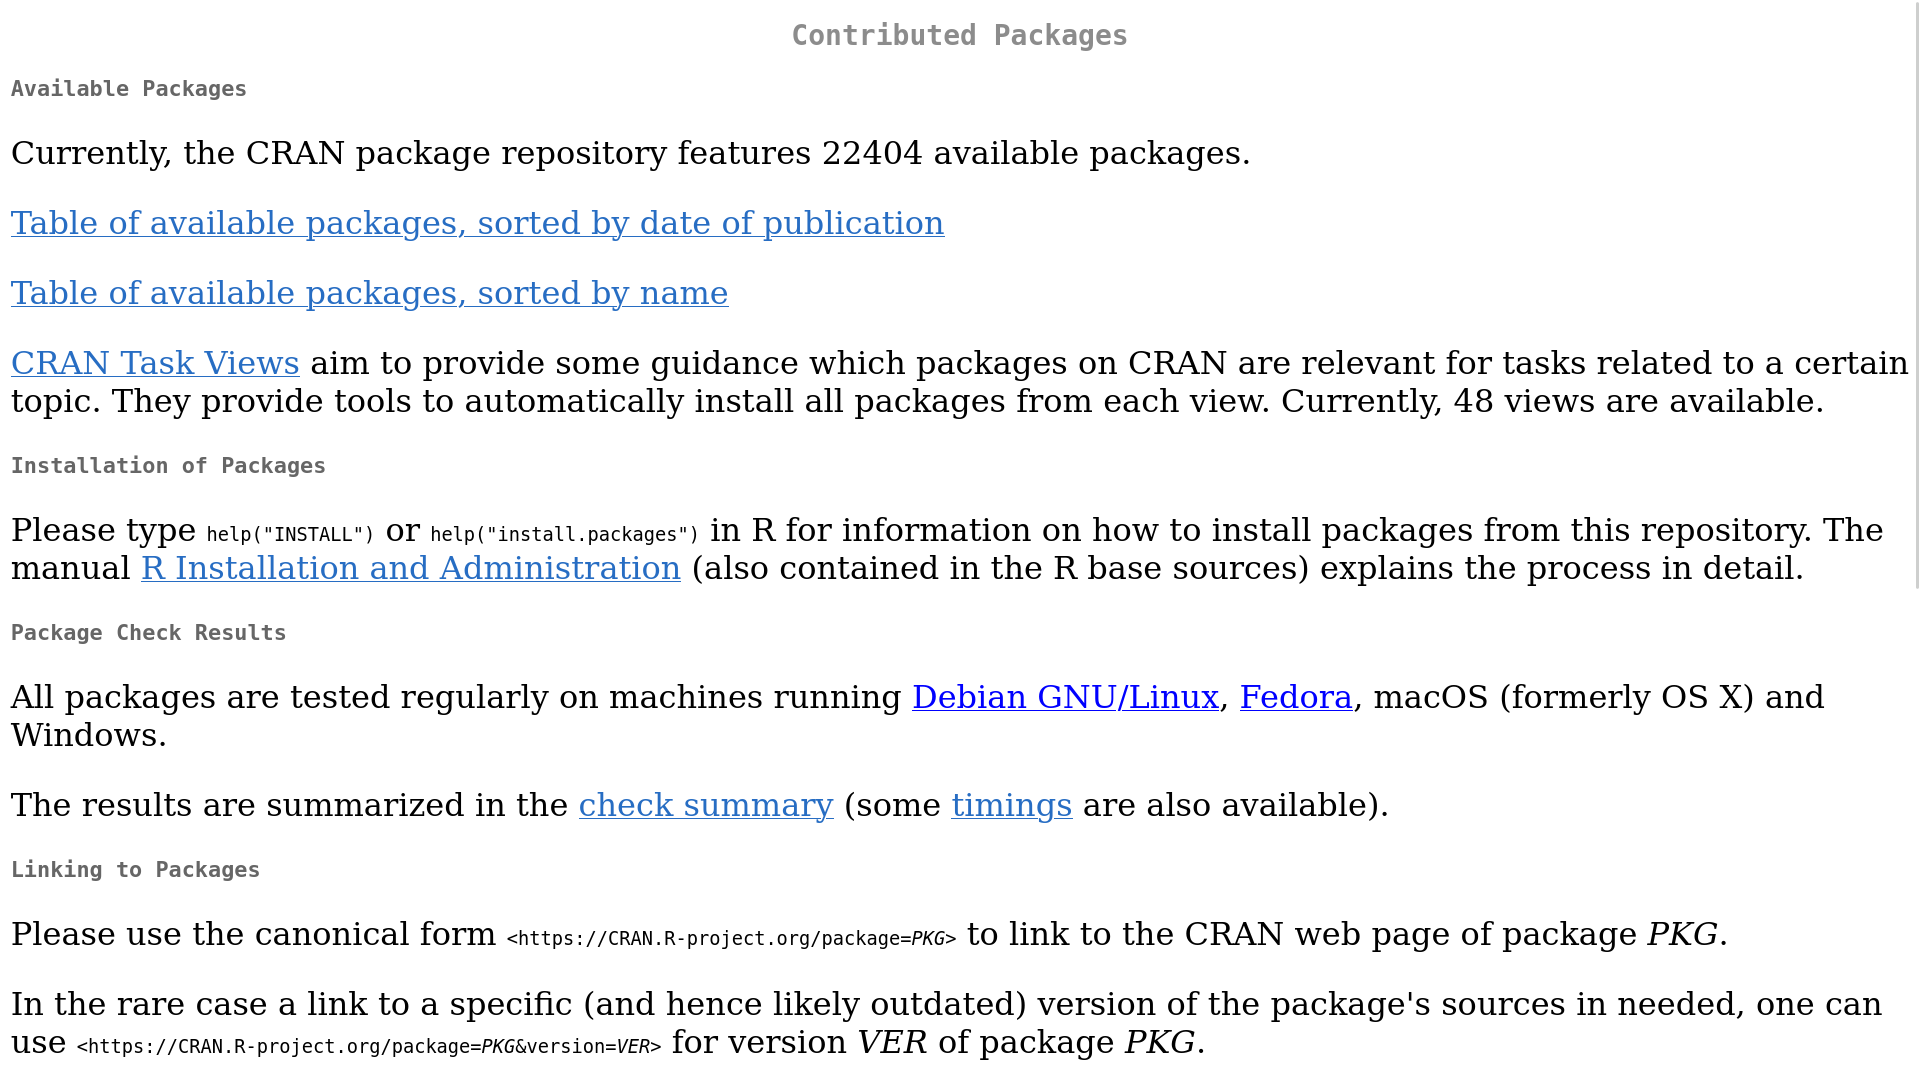
\includegraphics[keepaspectratio]{includes/page_r_scrape_new.png}}

}

\subcaption{\label{fig-page_contents}}

\end{minipage}%
%
\begin{minipage}{0.50\linewidth}

\centering{

\pandocbounded{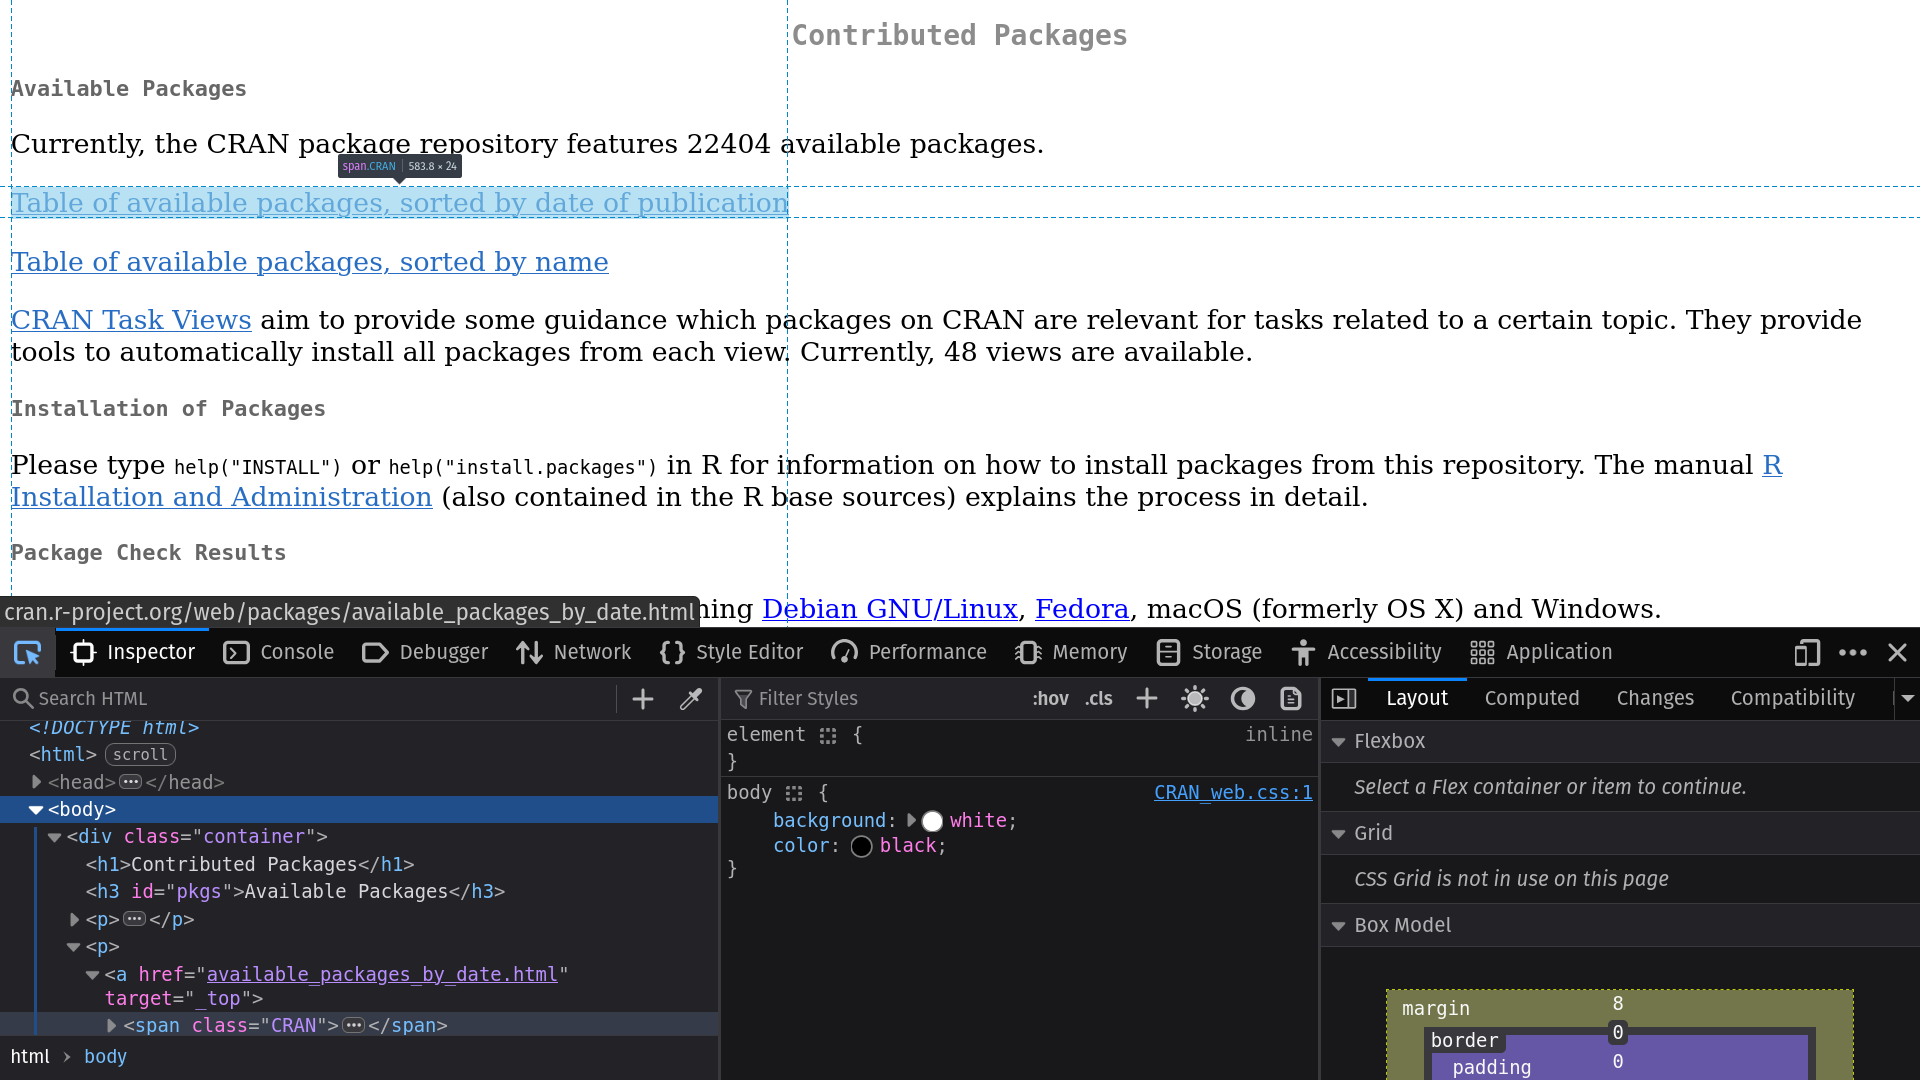
\includegraphics[keepaspectratio]{includes/new_webtools_r_scrape.png}}

}

\subcaption{\label{fig-page_contents_devtools}}

\end{minipage}%

\caption{\label{fig-pages_scrape}A Figura~\ref{fig-page_contents} exibe
a página que está sendo raspada, enquanto a
Figura~\ref{fig-page_contents_devtools} mostra a mesma página com um
exemplo do uso das ferramentas de desenvolvedor do Firefox.}

\end{figure}%

\vspace{12pt}

Com a execução do comando anterior, o conteúdo da página mostrada na
Figura~\ref{fig-page_contents} será carregado, permitindo a extração das
informações contidas em seu HTML. Se o comando \texttt{fetch} obter
êxito, a saída incluirá o código de status HTTP \texttt{200}, indicando
que a requisição foi bem sucedida. Abaixo, segue um exemplo desse
resultado:

\begin{Shaded}
\begin{Highlighting}[]
\ExtensionTok{In} \PreprocessorTok{[}\SpecialStringTok{1}\PreprocessorTok{]}\NormalTok{: fetch}\ErrorTok{(}\StringTok{"https://cran.r{-}project.org/web/packages/index.html"}\KeywordTok{)}
\ExtensionTok{2025{-}03{-}03}\NormalTok{ 08:04:24 }\PreprocessorTok{[}\SpecialStringTok{scrapy.core.engine}\PreprocessorTok{]}\NormalTok{ INFO: Spider opened}
\ExtensionTok{2025{-}03{-}03}\NormalTok{ 08:04:27 }\PreprocessorTok{[}\SpecialStringTok{scrapy.core.engine}\PreprocessorTok{]}\NormalTok{ DEBUG: Crawled }\ErrorTok{(}\ExtensionTok{200}\KeywordTok{)} \OperatorTok{\textless{}}\NormalTok{GET}
\ExtensionTok{https://cran.r{-}project.org/robots.txt}\OperatorTok{\textgreater{}} \ErrorTok{(}\ExtensionTok{referer:}\NormalTok{ None}\KeywordTok{)}
\ExtensionTok{2025{-}03{-}03}\NormalTok{ 08:04:28 }\PreprocessorTok{[}\SpecialStringTok{scrapy.core.engine}\PreprocessorTok{]}\NormalTok{ DEBUG: Crawled }\ErrorTok{(}\ExtensionTok{200}\KeywordTok{)} \OperatorTok{\textless{}}\NormalTok{GET}
\ExtensionTok{https://cran.r{-}project.org/web/packages/index.html}\OperatorTok{\textgreater{}} \ErrorTok{(}\ExtensionTok{referer:}\NormalTok{ None}\KeywordTok{)}
\end{Highlighting}
\end{Shaded}

Após a execução do comando \texttt{fetch}, o conteúdo da página ficará
armazenado no objeto \texttt{response}, que está disponível nativamente
no shell. Por exemplo, para visualizar o HTML da página, basta executar
\texttt{response.body}. A partir dessa resposta, é possível analisar a
estrutura da página e configurar o seletor para extrair apenas os dados
desejados. No entanto, para facilitar ainda mais esse trabalho,
navegadores como
\href{https://www.mozilla.org/pt-BR/firefox/}{\textbf{Firefox}} oferecem
ferramentas de desenvolvedor que permitem inspecionar a estrutura da
página, como pode ser visto na Figura~\ref{fig-page_contents_devtools}.
Para acessar essa ferramenta no
\href{https://www.mozilla.org/pt-BR/firefox/}{\textbf{Firefox}}, basta
utilizar o atalho \texttt{Ctrl+Shift+I}.

\begin{Shaded}
\begin{Highlighting}[]
\CommentTok{\textless{}!{-}{-}PARTE DO CONTEÚDO DA PÁGINA{-}{-}\textgreater{}}

\DataTypeTok{\textless{}!DOCTYPE}\NormalTok{ html}\DataTypeTok{\textgreater{}}
\DataTypeTok{\textless{}}\KeywordTok{html}\DataTypeTok{\textgreater{}}
\DataTypeTok{\textless{}}\KeywordTok{head}\DataTypeTok{\textgreater{}}
    \DataTypeTok{\textless{}}\KeywordTok{title}\DataTypeTok{\textgreater{}}\NormalTok{CRAN: Contributed Packages}\DataTypeTok{\textless{}/}\KeywordTok{title}\DataTypeTok{\textgreater{}}
    \DataTypeTok{\textless{}}\KeywordTok{link}\OtherTok{ rel}\OperatorTok{=}\StringTok{"stylesheet"}\OtherTok{ type}\OperatorTok{=}\StringTok{"text/css"}\OtherTok{ href}\OperatorTok{=}\StringTok{"../CRAN\_web.css"}\DataTypeTok{/\textgreater{}}
    \DataTypeTok{\textless{}}\KeywordTok{meta}\OtherTok{ http{-}equiv}\OperatorTok{=}\StringTok{"Content{-}Type"}
\OtherTok{     content}\OperatorTok{=}\StringTok{"text/html; charset=utf{-}8"}\DataTypeTok{/\textgreater{}}
    \DataTypeTok{\textless{}}\KeywordTok{meta}\OtherTok{ name}\OperatorTok{=}\StringTok{"viewport"}\OtherTok{ content}\OperatorTok{=}\StringTok{"width=device{-}width,}
\StringTok{     initial{-}scale=1.0, user{-}scalable=yes"}\DataTypeTok{/\textgreater{}}
\DataTypeTok{\textless{}/}\KeywordTok{head}\DataTypeTok{\textgreater{}}
\DataTypeTok{\textless{}}\KeywordTok{body}\DataTypeTok{\textgreater{}}
    \DataTypeTok{\textless{}}\KeywordTok{div}\OtherTok{ class}\OperatorTok{=}\StringTok{"container"}\DataTypeTok{\textgreater{}}
        \DataTypeTok{\textless{}}\KeywordTok{h1}\DataTypeTok{\textgreater{}}\NormalTok{Contributed Packages}\DataTypeTok{\textless{}/}\KeywordTok{h1}\DataTypeTok{\textgreater{}}

        \DataTypeTok{\textless{}}\KeywordTok{h3}\OtherTok{ id}\OperatorTok{=}\StringTok{"pkgs"}\DataTypeTok{\textgreater{}}\NormalTok{Available Packages}\DataTypeTok{\textless{}/}\KeywordTok{h3}\DataTypeTok{\textgreater{}}
        \DataTypeTok{\textless{}}\KeywordTok{p}\DataTypeTok{\textgreater{}}
\NormalTok{            Currently, the CRAN package repository features}
\NormalTok{            22127 available packages.}
        \DataTypeTok{\textless{}/}\KeywordTok{p}\DataTypeTok{\textgreater{}}
\NormalTok{        ...}
    \DataTypeTok{\textless{}/}\KeywordTok{div}\DataTypeTok{\textgreater{}}
\DataTypeTok{\textless{}/}\KeywordTok{body}\DataTypeTok{\textgreater{}}
\DataTypeTok{\textless{}/}\KeywordTok{html}\DataTypeTok{\textgreater{}}
\end{Highlighting}
\end{Shaded}

Após inspecionar a página, observa-se que existem elementos
\texttt{\textless{}a\textgreater{}} no corpo do HTML, cada um com um
atributo \texttt{href} associado. Os \texttt{href} serão necessários
para realizar a paginação e coletar os pacotes ordenados por data de
publicação. Para extrair os \texttt{href}, basta executar no shell o
comando
\texttt{response.css("a{[}target=\_top{]}\ ::attr(href)").get()}. Esse
comando utiliza seletores \texttt{CSS} para extrair o primeiro
\texttt{href} de um elemento \texttt{\textless{}a\textgreater{}} que
possui o atributo \texttt{target="\_top"}. Se for necessário extrair
todos os \texttt{href}, basta substituir o método \texttt{.get()} por
\texttt{.getall()}, o que retornará todos os valores correspondentes.

\vspace{12pt}

Com a execução do comando, é extraída uma string que será usada para
realizar a paginação, chamada
\texttt{\textquotesingle{}available\_packages\_by\_date.html\textquotesingle{}}.
O \texttt{\textquotesingle{}index.html\textquotesingle{}} que está na
string do atributo \texttt{start\_urls} deverá ser substituído pela
string obtida, direcionando para a página de pacotes ordenados por data
de publicação. Agora, com esse \texttt{href}, é possível utilizar o
shell e executar o comando \texttt{fetch} na url
\url{https://cran.r-project.org/web/packages/available_packages_by_date.html}
para carregar o conteúdo da página com a tabela de todos os pacotes
ordenados por data.

\vspace{12pt}

A nova página contém uma tabela com todos os pacotes, ordenados por
data, juntamente com suas descrições. Cada data, nome de pacote e
descrição estão contidos dentro do elemento
\texttt{\textless{}tr\textgreater{}} no HTML. Para selecionar todos os
textos presentes nesse elemento, basta executar o comando
\texttt{response.css("tr\ ::text").getall()}. Após a execução, será
gerada uma lista de strings com as informações de todos os pacotes. No
entanto, essa lista pode conter algumas strings vazias, que precisam ser
removidas. O código a seguir apresenta todos os seletores utilizados até
agora no shell, agora integrados ao spider, para dar início ao processo
de raspagem dos dados:

\begin{Shaded}
\begin{Highlighting}[]
\ImportTok{import}\NormalTok{ scrapy}


\KeywordTok{class}\NormalTok{ PackagescraperSpider(scrapy.Spider):}
\NormalTok{    name }\OperatorTok{=} \StringTok{"packagescraper"}
\NormalTok{    allowed\_domains }\OperatorTok{=}\NormalTok{ [}\StringTok{"cran.r{-}project.org"}\NormalTok{]}
\NormalTok{    start\_urls }\OperatorTok{=}\NormalTok{ [}\StringTok{"https://cran.r{-}project.org/web/packages/index.html"}\NormalTok{]}

    \KeywordTok{def}\NormalTok{ parse(}\VariableTok{self}\NormalTok{, response):}
\NormalTok{        href }\OperatorTok{=}\NormalTok{ response.css(}\StringTok{"a[target=\_top] ::attr(href)"}\NormalTok{).get()}
\NormalTok{        follow\_url }\OperatorTok{=}\NormalTok{ (}
          \VariableTok{self}\NormalTok{.start\_urls[}\DecValTok{0}\NormalTok{].replace(}\StringTok{"index.html"}\NormalTok{, }\StringTok{""}\NormalTok{) }\OperatorTok{+}\NormalTok{ href}
\NormalTok{        )}

        \ControlFlowTok{yield}\NormalTok{ response.follow(}
\NormalTok{            follow\_url,}
\NormalTok{            callback}\OperatorTok{=}\VariableTok{self}\NormalTok{.parse\_packages\_info,}
\NormalTok{            dont\_filter}\OperatorTok{=}\VariableTok{True}
\NormalTok{        )}

    \KeywordTok{def}\NormalTok{ parse\_packages\_info(}\VariableTok{self}\NormalTok{, response):}
\NormalTok{        get\_all\_tr }\OperatorTok{=}\NormalTok{ response.css(}\StringTok{"tr ::text"}\NormalTok{).getall()}
\NormalTok{        packages\_element }\OperatorTok{=}\NormalTok{ [}
\NormalTok{          x }\ControlFlowTok{for}\NormalTok{ x }\KeywordTok{in}\NormalTok{ get\_all\_tr }\ControlFlowTok{if}\NormalTok{ x.strip() }\OperatorTok{!=} \StringTok{""}
\NormalTok{        ][}\DecValTok{3}\NormalTok{:]}

\NormalTok{        pub\_date }\OperatorTok{=}\NormalTok{ packages\_element[::}\DecValTok{3}\NormalTok{]}
\NormalTok{        packs\_name }\OperatorTok{=}\NormalTok{ packages\_element[}\DecValTok{1}\NormalTok{::}\DecValTok{3}\NormalTok{]}
\NormalTok{        desc\_packs }\OperatorTok{=}\NormalTok{ packages\_element[}\DecValTok{2}\NormalTok{::}\DecValTok{3}\NormalTok{]}

        \ControlFlowTok{for}\NormalTok{ i }\KeywordTok{in} \BuiltInTok{zip}\NormalTok{(pub\_date, packs\_name, desc\_packs):}
            \ControlFlowTok{yield}\NormalTok{ \{}
                \StringTok{"publication\_date"}\NormalTok{: i[}\DecValTok{0}\NormalTok{],}
                \StringTok{"package\_name"}\NormalTok{: i[}\DecValTok{1}\NormalTok{],}
                \StringTok{"description\_packs"}\NormalTok{: i[}\DecValTok{2}\NormalTok{],}
\NormalTok{            \}}
\end{Highlighting}
\end{Shaded}

O código contém a mesma classe mostrada anteriormente no
\texttt{packagescraper.py}, mas agora inclui os seletores analisados no
shell e outras modificações. Por exemplo, o método
\texttt{parse(self,\ response)}, apresentado anteriormente, é
responsável por capturar o link que leva à tabela de pacotes. Esse link
é extraído utilizando o seletor definido anteriormente no shell. Em
seguida, esse link é concatenado à url base para formar a url completa
que será seguida pelo spider. O método \texttt{response.follow()} é
então usado para acessar a nova página e chamar o método
\texttt{parse\_packages\_info}, que continuará o processo de raspagem.

\vspace{12pt}

Dentro do método \texttt{parse\_packages\_info}, todos os textos
contidos nos elementos \texttt{\textless{}tr\textgreater{}} são
coletados com \texttt{response.css("tr\ ::text").getall()}. Como essa
extração pode incluir strings vazias, é aplicado um \texttt{.strip()} em
cada elemento da lista e removidos aqueles que resultam em uma string
vazia. Além disso, os primeiros três elementos são ignorados, pois não
contêm informações relevantes, apenas o cabeçalho da tabela.

\vspace{12pt}

Após a limpeza, os dados são organizados em três listas:
\texttt{pub\_date}, \texttt{packs\_name} e \texttt{desc\_packs}. Cada
uma delas recebe elementos específicos da lista filtrada, onde,
\texttt{pub\_date} contém as datas de publicação dos pacotes,
\texttt{packs\_name} contém os nomes dos pacotes e \texttt{desc\_packs}
contém as descrições dos pacotes.

\vspace{12pt}

Por fim, a função \texttt{zip(pub\_date,\ packs\_name,\ desc\_packs)}
permite iterar sobre as três listas simultaneamente, gerando um
dicionário com as chaves \texttt{publication\_date},
\texttt{package\_name} e \texttt{description\_packs}. Esse dicionário é
então passado para o \texttt{yield}, permitindo que
\href{https://docs.scrapy.org/en/latest}{\textbf{Scrapy}} armazene os
dados no formato desejado.

\vspace{12pt}

Com esse código, os dados coletados podem ser salvos em diferentes
formatos, como \texttt{.json} ou \texttt{.csv}, ao executar o spider.
Por exemplo, para salvar os dados como \texttt{.csv}, basta executar no
terminal o comando
\texttt{scrapy\ crawl\ -o\ packages.csv\ packagescraper}. Ao executar
esse comando, será salvo um arquivo chamado \texttt{packages.csv},
contendo todos os dados coletados do site alvo.

\vspace{12pt}

O exemplo apresentado aqui é bastante simples. No entanto, dependendo
das necessidades do projeto, pode ser necessário utilizar outras
ferramentas do
\href{https://docs.scrapy.org/en/latest}{\textbf{Scrapy}}. O código
completo para a raspagem de dados de imóveis pode ser acessado em
\url{https://github.com/cowvin0/tcc_realestate/tree/main/scrapy_zap}.
Esse código pode servir como material complementar ao que foi
apresentado neste texto, pois foram adicionadas mais funcionalidades
durante a coleta dos dados, atendendo a necessidades específicas do
projeto.

\subsection{Exemplo de web scraping em
R}\label{exemplo-de-web-scraping-em-r}

~~~Agora que a estrutura do site é conhecida e a inspeção dos dados de
interesse foi feita utilizando as ferramentas de desenvolvedor do
\href{https://www.mozilla.org/pt-BR/firefox/}{\textbf{Firefox}}, o
exemplo em R será mais direto. Neste exemplo, utiliza-se o pacote
\href{https://rvest.tidyverse.org/}{\textbf{rvest}},
\href{https://dplyr.tidyverse.org/}{\textbf{dplyr}} para criar a tabela
com as informações coletadas, e
\href{https://purrr.tidyverse.org/}{\textbf{purrr}}, que é um pacote de
\textbf{R} voltado para programação funcional. O código utilizado para a
extração pode ser visualizado abaixo:

\begin{Shaded}
\begin{Highlighting}[]
\FunctionTok{library}\NormalTok{(rvest)}
\FunctionTok{library}\NormalTok{(dplyr)}
\FunctionTok{library}\NormalTok{(purrr)}

\NormalTok{base\_url }\OtherTok{\textless{}{-}} \StringTok{"https://cran.r{-}project.org/web/packages/"}

\NormalTok{first\_package\_link }\OtherTok{\textless{}{-}} \FunctionTok{read\_html}\NormalTok{(}\FunctionTok{paste0}\NormalTok{(base\_url, }\StringTok{"index.html"}\NormalTok{)) }\SpecialCharTok{|\textgreater{}}
    \FunctionTok{html\_elements}\NormalTok{(}\StringTok{"a[target=\_top]"}\NormalTok{) }\SpecialCharTok{|\textgreater{}}
    \FunctionTok{html\_attr}\NormalTok{(}\StringTok{"href"}\NormalTok{) }\SpecialCharTok{|\textgreater{}}
    \FunctionTok{first}\NormalTok{()}

\NormalTok{package\_url }\OtherTok{\textless{}{-}} \FunctionTok{paste0}\NormalTok{(base\_url, first\_package\_link)}
\NormalTok{package\_page }\OtherTok{\textless{}{-}} \FunctionTok{read\_html}\NormalTok{(package\_url)}

\NormalTok{packages\_info }\OtherTok{\textless{}{-}}\NormalTok{ package\_page }\SpecialCharTok{|\textgreater{}}
    \FunctionTok{html\_elements}\NormalTok{(}\StringTok{"tr"}\NormalTok{) }\SpecialCharTok{|\textgreater{}}
    \FunctionTok{html\_text2}\NormalTok{() }\SpecialCharTok{|\textgreater{}}
    \FunctionTok{tail}\NormalTok{(}\SpecialCharTok{{-}}\DecValTok{1}\NormalTok{) }\SpecialCharTok{|\textgreater{}}
    \FunctionTok{map}\NormalTok{(}\SpecialCharTok{\textasciitilde{}} \FunctionTok{strsplit}\NormalTok{(.x, }\StringTok{"}\SpecialCharTok{\textbackslash{}t}\StringTok{"}\NormalTok{)[[}\DecValTok{1}\NormalTok{]])}

\NormalTok{packages\_df }\OtherTok{\textless{}{-}} \FunctionTok{tibble}\NormalTok{(}
    \AttributeTok{publication\_date =} \FunctionTok{map\_chr}\NormalTok{(packages\_info, }\DecValTok{1}\NormalTok{),}
    \AttributeTok{package\_name =} \FunctionTok{map\_chr}\NormalTok{(packages\_info, }\DecValTok{2}\NormalTok{),}
    \AttributeTok{description\_packs =} \FunctionTok{map\_chr}\NormalTok{(packages\_info, }\DecValTok{3}\NormalTok{)}
\NormalTok{)}
\end{Highlighting}
\end{Shaded}

Após carregar os pacotes necessários, o código define a url base do CRAN
e acessa a página inicial, que contém diversas informações sobre os
pacotes de \textbf{R}. Em seguida, o código extrai o primeiro link do
atributo \texttt{href} presente na página e constrói a url completa para
acessar a página com os pacotes ordenados por data de publicação.

\vspace{12pt}

Depois de carregar o conteúdo da página, o código busca as informações
contidas nos elementos \texttt{\textless{}tr\textgreater{}} da tabela
exibida no site. Os textos são extraídos e processados para remover o
cabeçalho. Em seguida, as informações são separadas em colunas distintas
utilizando a função \texttt{strsplit()}, que divide em uma lista os
dados de data de publicação, nome do pacote e descrição do pacote.

\vspace{12pt}

Por fim, os dados são organizados em um \texttt{tibble}, onde cada linha
contém a data de publicação, o nome do pacote e sua descrição. O uso da
função \texttt{map\_chr} do pacote
\href{https://purrr.tidyverse.org/}{\textbf{purrr}} garante que os
valores sejam extraídos retornando vetores de caracteres com cada uma
das informações. Ao final, ao salvar os dados do \texttt{tibble},
obtém-se a base de dados final construída, contendo a data de
publicação, o nome do pacote e sua descrição, conforme ilustrado na
Figura~\ref{fig-tabela_scrape}.

\begin{figure}

\centering{

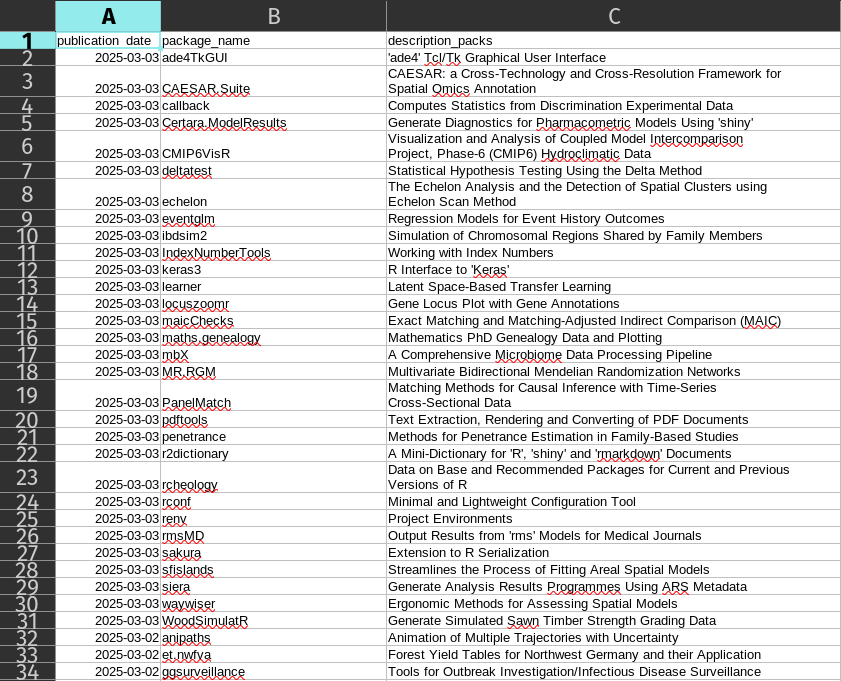
\includegraphics[width=4.6875in,height=2.60417in]{includes/scraped_table.png}

}

\caption{\label{fig-tabela_scrape}Dados obtidos a partir do web
scraping.}

\end{figure}%

\vspace{12pt}

Assim como no exemplo apresentado em \textbf{Python}, o projeto de
raspagem pode ser adaptado de acordo com as necessidades e as
informações que precisam ser coletadas. Ou seja, embora os exemplos
fornecidos sejam simples, dependendo das características do site, outras
funcionalidades podem ser adicionadas, como clicar em botões, rolar a
página automaticamente para carregar conteúdos dinâmicos, entre outras
ações.

\vspace{12pt}

Portanto, chega ao fim a descrição das tecnologias utilizadas para a
obtenção dos dados, com exemplos de raspagem em \textbf{R} e
\textbf{Python}. No entanto, a linguagem \textbf{Python}, em particular,
continuou sendo empregada em outras etapas deste trabalho, como na
modelagem dos valores de imóveis. Dessa forma, os próximos recursos
apresentados serão aqueles utilizados especificamente para a modelagem e
visualização dos resultados.

\section{Recursos utilizados para modelagem e visualização dos
resultados}\label{recursos-utilizados-para-modelagem-e-visualizauxe7uxe3o-dos-resultados}

~~~Com os dados coletados, a etapa de modelagem dos valores de imóveis
torna-se essencial para converter essas informações em entendimentos
relevantes e aplicáveis. Essa etapa permite identificar padrões de
comportamento entre as variáveis que influenciam os valores
imobiliários, além de determinar quais fatores exercem maior impacto
sobre esses valores. Para chegar a esses resultados, foram utilizadas
bibliotecas desenvolvidas em \textbf{Python}, como
\href{https://scikit-learn.org/stable/}{\textbf{scikit-learn}}
(PEDREGOSA, F. et al., 2011),
\href{https://pandas.pydata.org/}{\textbf{pandas}} (TEAM, 2020),
empregada para a manipulação das bases de dados utilizadas neste
trabalho, \href{https://numpy.org/}{\textbf{numpy}} (HARRIS et al.,
2020), voltada para computação numérica, entre outras.

\vspace{12pt}

O \href{https://scikit-learn.org/stable/}{\textbf{scikit-learn}} é uma
das bibliotecas de aprendizado de máquina mais populares em
\textbf{Python}. Ela oferece uma extensa coleção de algoritmos para
tarefas como classificação, regressão, clusterização, além de
ferramentas para pré-processamento de dados, validação cruzada e seleção
de modelos. O projeto teve início no Google Summer of Code como uma
iniciativa do engenheiro francês David Cournapeau. O
\href{https://scikit-learn.org/stable/}{\textbf{scikit-learn}} foi
criado como uma ferramenta baseada na biblioteca
\href{https://scipy.org/}{\textbf{SciPy}} (VIRTANEN et al., 2020), que é
voltada para computação científica e cálculo numérico em
\textbf{Python}.

\vspace{12pt}

Uma das funcionalidades mais úteis do
\href{https://scikit-learn.org/stable/}{\textbf{scikit-learn}} é o uso
de pipelines para transformar dados. As pipelines permitem combinar
etapas de pré-processamento e ajuste de modelos em um único fluxo
organizado. Isso não apenas simplifica o código, mas também assegura que
as transformações aplicadas aos dados de treinamento sejam
automaticamente replicadas nos dados de teste ou em novos dados. Além de
serem úteis para tarefas mais simples, como normalização de variáveis,
as pipelines também permitem a inclusão de etapas personalizadas para
lidar com cenários mais complexos, como tratamentos avançados de dados
ou integração com ferramentas externas.

\vspace{12pt}

O exemplo abaixo ilustra uma pipeline para pré-processamento e
modelagem. As variáveis numéricas passam por padronização, enquanto as
variáveis categóricas são transformadas em variáveis binárias utilizando
codificação one-hot. Por fim, os dados processados alimentam um
algoritmo de Random Forest para regressão:

\begin{Shaded}
\begin{Highlighting}[]
\ImportTok{import}\NormalTok{ numpy }\ImportTok{as}\NormalTok{ np}
\ImportTok{from}\NormalTok{ sklearn.model\_selection }\ImportTok{import}\NormalTok{ train\_test\_split}
\ImportTok{from}\NormalTok{ sklearn.pipeline }\ImportTok{import}\NormalTok{ Pipeline}
\ImportTok{from}\NormalTok{ sklearn.compose }\ImportTok{import}\NormalTok{ ColumnTransformer}
\ImportTok{from}\NormalTok{ sklearn.preprocessing }\ImportTok{import}\NormalTok{ StandardScaler, OneHotEncoder}
\ImportTok{from}\NormalTok{ sklearn.ensemble }\ImportTok{import}\NormalTok{ RandomForestRegressor}

\NormalTok{X\_train, X\_test, y\_train, y\_test }\OperatorTok{=}\NormalTok{ train\_test\_split(}
\NormalTok{    X, y,}
\NormalTok{    test\_size}\OperatorTok{=}\FloatTok{0.2}\NormalTok{,}
\NormalTok{    random\_state}\OperatorTok{=}\DecValTok{42}
\NormalTok{)}

\NormalTok{numerical\_features }\OperatorTok{=}\NormalTok{ X.select\_dtypes(include}\OperatorTok{=}\NormalTok{np.number).columns}
\NormalTok{categorical\_features }\OperatorTok{=}\NormalTok{ X.select\_dtypes(include}\OperatorTok{=}\BuiltInTok{object}\NormalTok{).columns}

\NormalTok{pipeline }\OperatorTok{=}\NormalTok{ Pipeline([}
\NormalTok{    (}\StringTok{\textquotesingle{}preprocessor\textquotesingle{}}\NormalTok{, ColumnTransformer([}
\NormalTok{        (}\StringTok{\textquotesingle{}num\textquotesingle{}}\NormalTok{, StandardScaler(), numerical\_features),}
\NormalTok{        (}\StringTok{\textquotesingle{}cat\textquotesingle{}}\NormalTok{, OneHotEncoder(), categorical\_features)}
\NormalTok{    ])),}
\NormalTok{    (}\StringTok{\textquotesingle{}model\textquotesingle{}}\NormalTok{, RandomForestRegressor(}
\NormalTok{        n\_estimators}\OperatorTok{=}\DecValTok{100}\NormalTok{,}
\NormalTok{        random\_state}\OperatorTok{=}\DecValTok{42}
\NormalTok{    ))}
\NormalTok{])}

\NormalTok{pipeline.fit(X\_train, y\_train)}
\end{Highlighting}
\end{Shaded}

Outra etapa fundamental no processo de aprendizado de máquina, além do
pré-processamento dos dados e do ajuste do algoritmo, é a otimização dos
hiperparâmetros. O
\href{https://scikit-learn.org/stable/}{\textbf{scikit-learn}} oferece
algumas ferramentas para essa tarefa, mas elas possuem funcionalidades
mais básicas e podem ser limitadas para cenários mais complexos. Dessa
forma, de forma complementar, esse trabalho utilizou a biblioteca
\href{https://optuna.org/}{\textbf{Optuna}} (AKIBA et al., 2019), que é
uma biblioteca que contém uma grande quantidade de algoritmos para
otimização, como, por exemplo, métodos de otimização bayesiana. No
entanto, inicialmente foram ajustados alguns modelos utilizando a
biblioteca \href{https://pycaret.org/}{\textbf{pycaret}}, com o objetivo
de explorar quais métodos apresentariam melhor desempenho.

\vspace{12pt}

Além das funcionalidades de otimização, o
\href{https://optuna.org/}{\textbf{Optuna}} também oferece ferramentas
para analisar o comportamento da função objetivo durante o processo de
otimização e identificar os hiperparâmetros mais relevantes. Uma dessas
ferramentas é a função \texttt{plot\_param\_importances}, que gera um
gráfico destacando a importância relativa de cada hiperparâmetro. Além
disso, como o \texttt{plot\_param\_importances} utiliza a biblioteca
\href{https://matplotlib.org/}{\textbf{Matplotlib}} (HUNTER, 2007), os
gráficos gerados podem ser personalizados pelo usuário.

\vspace{12pt}

Vale destacar que bibliotecas como o
\href{https://matplotlib.org/}{\textbf{Matplotlib}} e o
\href{https://seaborn.pydata.org/}{\textbf{seaborn}} (WASKOM, 2021)
desempenharam um papel fundamental na geração dos gráficos e na
visualização dos dados apresentados neste trabalho. Essas ferramentas
foram indispensáveis para a análise exploratória e a apresentação dos
resultados de forma clara e compreensível. Além dessas bibliotecas,
também foram utilizados recursos voltados para a análise do impacto e
das relações entre as variáveis e as previsões geradas pelos modelos.
Nesse contexto, destacam-se o
\href{https://shap.readthedocs.io/en/latest}{\textbf{SHAP}} (LUNDBERG;
LEE, 2017) e o
\href{https://lime-ml.readthedocs.io/en/latest/}{\textbf{LIME}}, que
fornecem explicações interpretáveis para os modelos de aprendizado de
máquina, e o próprio
\href{https://scikit-learn.org/stable/}{\textbf{scikit-learn}}, que foi
essencial para a criação dos gráficos de ICE (Individual Conditional
Expectation). Esses métodos serão detalhados na seção de metodologia
deste trabalho.

\vspace{12pt}

Vale ressaltar que algumas bibliotecas externas, baseadas na API do
\href{https://scikit-learn.org/stable/}{\textbf{scikit-learn}}, também
foram utilizadas neste trabalho. Entre elas, destacam-se a
\href{https://lightgbm.readthedocs.io/en/stable/}{\textbf{LightGBM}} (KE
et al., 2017) e a
\href{https://xgboost.readthedocs.io/en/stable/}{\textbf{XGBoost}}
(CHEN, T.; GUESTRIN, 2016), empregadas para a implementação de
algoritmos de aprendizado de máquina. Essas bibliotecas fornecem,
respectivamente, os algoritmos de gradient boosting LightGBM e Extreme
Gradient Boosting, reconhecidos por sua eficiência computacional e
desempenho em tarefas de modelagem preditiva.

\vspace{12pt}

Conclui-se, assim, a apresentação das ferramentas empregadas na
modelagem e visualização dos resultados. A seguir, serão descritas as
tecnologias utilizadas no desenvolvimento da aplicação final deste
trabalho. Vale destacar que o
\href{https://scikit-learn.org/stable/}{\textbf{scikit-learn}} continuou
desempenhando um papel relevante na aplicação, com sua pipeline sendo
serializada no formato \texttt{.pkl} por meio da biblioteca
\href{https://docs.python.org/3/library/pickle.html}{\textbf{pickle}}.
Essa biblioteca permitiu a reutilização da pipeline no
back-end\footnote{Back-end é a parte de um sistema ou aplicação
  responsável pelo processamento de dados, lógica e comunicação com
  bancos de dados e servidores, funcionando nos bastidores da interface
  com o usuário.} da aplicação, garantindo a consistência, eficiência do
processamento dos dados e predição do modelo para novos dados. Segue,
então, a descrição das ferramentas empregadas na construção da aplicação
final.

\section{Recursos utilizados para a criação da aplicação
final}\label{recursos-utilizados-para-a-criauxe7uxe3o-da-aplicauxe7uxe3o-final}

~~~A aplicação final foi desenvolvida com o objetivo de realizar
previsões de valores de imóveis e oferecer uma análise detalhada do
mercado imobiliário da cidade de João Pessoa. Além de integrar a
pipeline de machine learning criada durante a etapa de modelagem, a
aplicação também dispõe de funcionalidades interativas que permitem aos
usuários explorar os dados e visualizar os resultados de forma clara e
intuitiva. Para alcançar esses objetivos, foram empregadas tecnologias
para o desenvolvimento do front-end\footnote{Front-end é a parte de um
  sistema ou aplicação responsável pela interface gráfica e pela
  interação com o usuário.} e do back-end, que foram desenvolvidos em
\textbf{Python}.

\vspace{12pt}

O front-end da aplicação foi desenvolvido utilizando a biblioteca
\href{https://dash.plotly.com/}{\textbf{Dash}} (HOSSAIN, 2019), uma
ferramenta voltada para a criação de aplicativos web em \textbf{Python}.
Desenvolvida pela \href{https://plotly.com/}{\textbf{Plotly}} (INC.,
2015), a \href{https://dash.plotly.com/}{\textbf{Dash}} permite
construir interfaces gráficas completas sem a necessidade de
conhecimentos avançados em desenvolvimento web, integrando tecnologias
como \texttt{HTML}, \texttt{CSS} e \textbf{JavaScript} diretamente no
ambiente \textbf{Python}. Entre suas principais características,
destacam-se a facilidade de criar gráficos interativos, a integração com
bibliotecas populares como \href{https://plotly.com/}{\textbf{Plotly}} e
a capacidade de atualizar componentes de forma dinâmica por meio de suas
funções \texttt{callback}. A seguir, é apresentado um exemplo do uso da
função \texttt{callback}:

\begin{Shaded}
\begin{Highlighting}[]
\ImportTok{from}\NormalTok{ dash }\ImportTok{import}\NormalTok{ Dash, dcc, html, Output, Input}
\ImportTok{import}\NormalTok{ plotly.express }\ImportTok{as}\NormalTok{ px}
\ImportTok{import}\NormalTok{ pandas }\ImportTok{as}\NormalTok{ pd}

\NormalTok{df }\OperatorTok{=}\NormalTok{ pd.DataFrame(}
\NormalTok{    \{}
        \StringTok{"Categoria"}\NormalTok{: [}\StringTok{"A"}\NormalTok{, }\StringTok{"B"}\NormalTok{, }\StringTok{"C"}\NormalTok{],}
        \StringTok{"Valores"}\NormalTok{: [}\DecValTok{10}\NormalTok{, }\DecValTok{20}\NormalTok{, }\DecValTok{30}\NormalTok{]}
\NormalTok{    \}}
\NormalTok{)}

\NormalTok{app }\OperatorTok{=}\NormalTok{ Dash(}\VariableTok{\_\_name\_\_}\NormalTok{)}

\NormalTok{app.layout }\OperatorTok{=}\NormalTok{ html.Div(}
\NormalTok{    [}
\NormalTok{        dcc.Dropdown(}
            \BuiltInTok{id}\OperatorTok{=}\StringTok{"dropdown"}\NormalTok{,}
\NormalTok{            options}\OperatorTok{=}\NormalTok{[}
\NormalTok{                \{}\StringTok{"label"}\NormalTok{: cat, }\StringTok{"value"}\NormalTok{: cat\}}
                \ControlFlowTok{for}\NormalTok{ cat }\KeywordTok{in}\NormalTok{ df[}\StringTok{"Categoria"}\NormalTok{]}
\NormalTok{            ],}
\NormalTok{            value}\OperatorTok{=}\StringTok{"A"}\NormalTok{,}
\NormalTok{            clearable}\OperatorTok{=}\VariableTok{False}\NormalTok{,}
\NormalTok{        ),}
\NormalTok{        dcc.Graph(}\BuiltInTok{id}\OperatorTok{=}\StringTok{"graph"}\NormalTok{),}
\NormalTok{    ]}
\NormalTok{)}


\AttributeTok{@app.callback}\NormalTok{(Output(}\StringTok{"graph"}\NormalTok{, }\StringTok{"figure"}\NormalTok{), Input(}\StringTok{"dropdown"}\NormalTok{, }\StringTok{"value"}\NormalTok{))}
\KeywordTok{def}\NormalTok{ update\_graph(selected\_category):}
\NormalTok{    filtered\_df }\OperatorTok{=}\NormalTok{ df[df[}\StringTok{"Categoria"}\NormalTok{] }\OperatorTok{==}\NormalTok{ selected\_category]}
\NormalTok{    fig }\OperatorTok{=}\NormalTok{ px.bar(}
\NormalTok{        filtered\_df,}
\NormalTok{        x}\OperatorTok{=}\StringTok{"Categoria"}\NormalTok{,}
\NormalTok{        y}\OperatorTok{=}\StringTok{"Valores"}\NormalTok{,}
\NormalTok{        title}\OperatorTok{=}\SpecialStringTok{f"Valores da Categoria }\SpecialCharTok{\{}\NormalTok{selected\_category}\SpecialCharTok{\}}\SpecialStringTok{"}\NormalTok{,}
\NormalTok{    )}

    \ControlFlowTok{return}\NormalTok{ fig}


\ControlFlowTok{if} \VariableTok{\_\_name\_\_} \OperatorTok{==} \StringTok{"\_\_main\_\_"}\NormalTok{:}
\NormalTok{    app.run\_server(debug}\OperatorTok{=}\VariableTok{True}\NormalTok{)}
\end{Highlighting}
\end{Shaded}

Neste exemplo, o código permite que o usuário selecione um valor em um
menu suspenso, criado a partir da classe \texttt{Dropdown}, e exiba o
valor escolhido em um gráfico. Primeiramente, é criado um pequeno
conjunto de dados utilizando a biblioteca
\href{https://pandas.pydata.org/}{\textbf{pandas}}, contendo categorias
(A, B e C) e valores associados a elas. Em seguida, define-se o layout
da aplicação (\texttt{app.layout}), que consiste em um \texttt{Dropdown}
para selecionar uma categoria e um componente \texttt{Graph} para exibir
o gráfico correspondente. A lógica para atualizar o gráfico conforme a
seleção do usuário é implementada por meio da função \texttt{callback}.
O decorador \texttt{@app.callback} conecta o valor selecionado no
\texttt{Dropdown} (definido pela classe \texttt{Input}) ao gráfico
(definido pela classe \texttt{Output}). A função associada ao decorador
\texttt{callback}, chamada \texttt{update\_graph}, recebe como argumento
o valor escolhido no \texttt{Dropdown}, filtra o DataFrame com base na
categoria selecionada e gera um gráfico de barras utilizando a
biblioteca \href{https://plotly.com/}{\textbf{Plotly}}. Este gráfico é
então retornado para ser exibido no componente \texttt{Graph}.

\vspace{12pt}

Para o desenvolvimento do back-end da aplicação foi utilizado o
framework \href{https://fastapi.tiangolo.com/}{\textbf{FastAPI}}, uma
ferramenta moderna e eficiente para a criação de APIs em
\textbf{Python}. O
\href{https://fastapi.tiangolo.com/}{\textbf{FastAPI}} é conhecido por
sua alta performance, graças ao uso de tipagem estática e a sua
facilidade de suporte assíncrono, além de permitir a criação de APIs de
maneira rápida e simples. Além disso, integra-se facilmente com
bibliotecas como
\href{https://docs.pydantic.dev/latest/}{\textbf{Pydantic}} para
validação de dados e
\href{https://www.sqlalchemy.org/}{\textbf{SQLAlchemy}} (BAYER, 2012)
para interação e conexão com bancos de dados.

\vspace{12pt}

No projeto, o \href{https://www.sqlalchemy.org/}{\textbf{SQLAlchemy}}
foi utilizado para gerenciar a conexão com o banco de dados,
implementado com
\href{https://www.postgresql.org/}{\textbf{PostgreSQL}}, um sistema de
gerenciamento de banco de dados relacional amplamente reconhecido por
sua robustez e alto desempenho. Isso permitiu que os dados fossem
expostos na API e consumidos no front-end. Além disso, a API foi
responsável por expor a pipeline do modelo, possibilitando a realização
de previsões de valores imobiliários diretamente na aplicação. Não
obstante, os mapas da cidade de João Pessoa contidos na aplicação, foram
criados com a biblioteca
\href{https://python-visualization.github.io/folium/latest/}{\textbf{Folium}}
(PYTHON-VISUALIZATION, 2020) e
\href{https://www.dash-leaflet.com/}{\textbf{dash-leaflet}}.

\vspace{12pt}

O \href{https://www.docker.com/}{\textbf{Docker}} foi utilizado para
facilitar a execução e integração dos componentes da aplicação,
permitindo a criação de ambientes isolados e consistentes para o
front-end e o back-end. Por meio de containers, foi possível iniciar e
conectar ambos os serviços de forma simplificada, garantindo que a
aplicação funcionasse corretamente independentemente do ambiente em que
fosse executada. Com o uso do
\href{https://www.docker.com/}{\textbf{Docker}}, a configuração do
ambiente tornou-se reprodutível, escalável e de fácil manutenção. Além
disso, o banco de dados
\href{https://www.postgresql.org/}{\textbf{PostgreSQL}} foi criado a
partir do \href{https://www.docker.com/}{\textbf{Docker}}.

\vspace{12pt}

O \href{https://www.docker.com/}{\textbf{Docker}} é uma plataforma que
permite empacotar aplicações e suas dependências em unidades chamadas
containers, que podem ser executadas de maneira padronizada em qualquer
sistema que possua o \href{https://www.docker.com/}{\textbf{Docker}}
instalado. Isso elimina problemas comuns relacionados a diferenças de
ambiente e facilita o processo de desenvolvimento, teste e implantação
de aplicações.

\vspace{12pt}

Com as tecnologias mencionadas anteriormente e o modelo final obtido,
foi possível criar uma aplicação capaz de realizar previsões para os
imóveis da cidade de João Pessoa, além de proporcionar uma análise de
seu setor imobiliário. No entanto, o desenvolvimento de todo o código da
aplicação exigiu o uso de ferramentas que facilitassem sua escrita,
desenvolvimento e organização. Assim, a seguir serão apresentadas as
ferramentas utilizadas tanto para a implementação do código deste
trabalho quanto para a elaboração do documento final que o descreve.

\section{Recursos utilizados para escrita de código e de
documento}\label{recursos-utilizados-para-escrita-de-cuxf3digo-e-de-documento}

~~~O desenvolvimento deste trabalho foi realizado em um computador
equipado com processador AMD Ryzen 7 5800H (16 núcleos), 8 GB de memória
RAM, placa de vídeo GeForce GTX 1650 e um SSD NVMe de 256 GB, operando
sob o sistema Pop!\_OS 22.04 LTS. Embora a máquina ofereça um desempenho
geral satisfatório, a quantidade limitada de memória RAM apresentou
desafios em tarefas mais intensivas, como a otimização de
hiperparâmetros dos modelos. Essas tarefas frequentemente demandavam até
dois dias para sua conclusão e, em alguns casos, falhavam próximo ao
término devido ao alto consumo computacional. Dessa forma, a escolha das
ferramentas utilizadas para a escrita do código foram as que impactassem
o mínimo possível no desempenho do sistema.

\vspace{12pt}

O \href{https://code.visualstudio.com/}{\textbf{Visual Studio Code
(VSCode)}} foi a principal ferramenta utilizada para a escrita do código
neste trabalho. O \href{https://code.visualstudio.com/}{\textbf{VSCode}}
é um editor bastante leve e oferece suporte a diversas linguagens de
programação e permite integração com inúmeras tecnologias por meio de
suas extensões. Entre as extensões utilizadas, destaca-se o
\href{https://marketplace.visualstudio.com/items?itemName=vscodevim.vim}{\textbf{vscodevim}},
que incorpora os key mappings do editor de texto Vim, originalmente
criado por Bram Moolenaar e lançado em 2 de novembro de 1991. Além
disso, foram empregadas extensões específicas para as linguagens
\textbf{Python} e \textbf{R}, tendo como principal objetivo uma melhor
formatação de código, execução e identificação de possíveis erros.

\vspace{12pt}

Por exemplo, uma das extensões utilizadas para análise estática de
código em \textbf{Python} foi o
\href{https://marketplace.visualstudio.com/items?itemName=ms-pyright.pyright}{\textbf{Pyright}},
desenvolvido pela Microsoft. Essa ferramenta é projetada para detectar
erros durante o desenvolvimento e verificar a tipagem de código em
\textbf{Python}, contribuindo para a melhoria da qualidade e da
manutenção do programa. Outra ferramenta empregada foi o
\href{https://marketplace.visualstudio.com/items?itemName=ms-python.black-formatter}{\textbf{Black
Formatter}}, um formatador de código \textbf{Python}. Ele automatiza a
padronização do estilo de código, garantindo consistência e
legibilidade. Além disso, foi utilizado o
\href{https://marketplace.visualstudio.com/items?itemName=ms-python.flake8}{\textbf{Flake8}},
que analisa o código em busca de erros de sintaxe, problemas de estilo
com base no padrão \href{https://peps.python.org/pep-0008/}{\textbf{PEP
8}}, e outras questões, como redundâncias ou importações desnecessárias.
Por fim, também foi utilizada uma extensão mais geral de suporte à
linguagem \textbf{Python}, que oferece diversas funcionalidades, como
correção de código por meio da extensão
\href{https://marketplace.visualstudio.com/items?itemName=ms-python.debugpy}{\textbf{PythonDebugger}},
que utiliza a biblioteca
\href{https://pypi.org/project/debugpy/}{\textbf{debugpy}} para suporte
ao processo de debugging.

\vspace{12pt}

Para a elaboração deste documento, foi utilizado o
\href{https://quarto.org/}{\textbf{Quarto}} (ALLAIRE; DERVIEUX, 2024),
uma plataforma de publicação científica desenvolvida pela empresa Posit.
O \href{https://quarto.org/}{\textbf{Quarto}} é uma evolução do
RMarkdown e se destaca por sua capacidade de criar documentos de alta
qualidade que integram texto e código. Compatível com diversas
linguagens de programação, como \textbf{R}, \textbf{Python}, e outras,
essa ferramenta é extremamente versátil para análise de dados e geração
de relatórios. Com o \href{https://quarto.org/}{\textbf{Quarto}}, é
possível produzir relatórios, artigos, livros, apresentações e até
sites. Ele é amplamente adotado na comunidade científica, especialmente
entre usuários de \textbf{R}, e oferece suporte a Markdown e \LaTeX, o
que facilita a inclusão de fórmulas matemáticas, gráficos, tabelas e
outros elementos visuais. Além disso, os documentos gerados podem ser
exportados para diversos formatos, como HTML, PDF, MS Word, entre
outros. O \href{https://quarto.org/}{\textbf{Quarto}} também foi
utilizado por meio do
\href{https://code.visualstudio.com/}{\textbf{VSCode}}, com a sua
extensão disponível em \url{https://quarto.org/docs/tools/vscode.html}.

\vspace{12pt}

No contexto deste trabalho, o
\href{https://quarto.org/}{\textbf{Quarto}} foi utilizado para a
produção de todo o texto, garantindo conformidade com as normas da ABNT.
Sua capacidade de integrar texto, código e gráficos de maneira
organizada foi essencial para facilitar o desenvolvimento do documento.

\chapter{Algoritmos de Aprendizado de
Máquina}\label{algoritmos-de-aprendizado-de-muxe1quina}

~~~Neste capítulo, serão descritos os algoritmos de aprendizado de
máquina utilizados neste trabalho. Alguns dos métodos utilizados podem
fazer uso de diversos algoritmos ou modelos estatísticos. No entanto, o
foco principal e o mais utilizado foram as árvores de decisão,
especialmente em sua forma particular, as árvores de regressão. Assim,
os algoritmos descritos são métodos baseados em árvores.

\vspace{12pt}

Os métodos baseados em árvore envolvem a estratificação ou segmentação
do espaço dos preditores em várias regiões simples. Dessa forma, todos
os algoritmos utilizados neste trabalho partem dessa ideia. Portanto, o
primeiro a ser explicado será o de árvores de decisão, pois fundamenta
todos os outros algoritmos. Depois das árvores de decisão, serão
explicados os métodos ensemble e, por fim, diferentes variações do
método de gradient boosting.

\begin{longtable}[]{@{}
  >{\centering\arraybackslash}p{(\linewidth - 6\tabcolsep) * \real{0.5143}}
  >{\centering\arraybackslash}p{(\linewidth - 6\tabcolsep) * \real{0.1286}}
  >{\centering\arraybackslash}p{(\linewidth - 6\tabcolsep) * \real{0.1714}}
  >{\centering\arraybackslash}p{(\linewidth - 6\tabcolsep) * \real{0.1857}}@{}}
\caption{Métricas de ajuste na base de teste obtidas a partir da
avaliação de diversos modelos, utilizando validação cruzada K-Fold com K
= 20.}\label{tbl-testing_models}\tabularnewline
\toprule\noalign{}
\begin{minipage}[b]{\linewidth}\centering
Algoritmo
\end{minipage} & \begin{minipage}[b]{\linewidth}\centering
RMSE
\end{minipage} & \begin{minipage}[b]{\linewidth}\centering
R² (\%)
\end{minipage} & \begin{minipage}[b]{\linewidth}\centering
MAPE (\%)
\end{minipage} \\
\midrule\noalign{}
\endfirsthead
\toprule\noalign{}
\begin{minipage}[b]{\linewidth}\centering
Algoritmo
\end{minipage} & \begin{minipage}[b]{\linewidth}\centering
RMSE
\end{minipage} & \begin{minipage}[b]{\linewidth}\centering
R² (\%)
\end{minipage} & \begin{minipage}[b]{\linewidth}\centering
MAPE (\%)
\end{minipage} \\
\midrule\noalign{}
\endhead
\bottomrule\noalign{}
\endlastfoot
Random Forest Regressor & 0,26 & 85,75 & 1,39 \\
Extra Trees Regressor & 0,27 & 85,47 & 1,40 \\
Extreme Gradient Boosting & 0,27 & 85,27 & 1,47 \\
Light Gradient Boosting Machine & 0,27 & 84,63 & 1,53 \\
Gradient Boosting Regressor & 0,30 & 81,97 & 1,70 \\
K Neighbors Regressor & 0,31 & 80,05 & 1,69 \\
Linear Regression & 0,34 & 76,95 & 1,95 \\
Ridge Regression & 0,34 & 76,95 & 1,95 \\
Bayesian Ridge & 0,34 & 76,95 & 1,95 \\
Decision Tree Regressor & 0,36 & 73,74 & 1,78 \\
AdaBoost Regressor & 0,37 & 72,29 & 2,21 \\
Orthogonal Matching Pursuit & 0,43 & 62,62 & 2,47 \\
Huber Regressor & 0,58 & 29,90 & 3,14 \\
Lasso Regression & 0,62 & 21,97 & 3,64 \\
Elastic Net & 0,62 & 21,97 & 3,64 \\
Lasso Least Angle Regression & 0,62 & 21,97 & 3,64 \\
Dummy Regressor & 0,70 & -0,05 & 4,21 \\
Passive Aggressive Regressor & 2,42 & -1130,87 & 13,84 \\
Least Angle Regression & 5,08 & -97949,99 & 26,54 \\
\end{longtable}

A Tabela~\ref{tbl-testing_models} apresenta os resultados obtidos para
diferentes algoritmos, treinados inicialmente com o objetivo de
identificar quais métodos seriam utilizados para a predição dos valores
de imóvel. Observa-se que os melhores desempenhos, segundo as métricas
RMSE, \(R^2\) e MAPE, foram alcançados majoritariamente por modelos
baseados em árvores. O Random Forest Regressor, por exemplo, foi o
algoritmo que obteve o melhor resultado. Modelos como o Extra Trees
Regressor, Extreme Gradient Boosting, LightGBM e Gradient Boosting
Regressor também figuram entre os mais eficazes, superando
consistentemente os métodos lineares e outros algoritmos. Esses
resultados justificam a ênfase nos métodos baseados em árvores ao longo
do trabalho, visto que eles apresentam desempenho superior na tarefa de
predição considerada, tanto em termos de precisão quanto de robustez
frente a diferentes abordagens. Vale destacar que os modelos foram
ajustados após todas as etapa de processamento.

\section{Árvores de decisão}\label{uxe1rvores-de-decisuxe3o}

~~~Árvores de decisão podem ser utilizadas tanto para regressão quanto
para classificação. Elas servem de base para os modelos baseados em
árvores empregados neste trabalho, com foco especial nas árvores de
regressão\footnote{Uma árvore de regressão é um caso específico da
  árvore de decisão, mas para regressão.}. O processo de construção de
uma árvore se baseia no particionamento recursivo do espaço dos
preditores, onde cada particionamento é chamado de nó e o resultado
final é chamado de folha ou nó terminal. Em cada nó, é definida uma
condição e, caso essa condição seja satisfeita, o resultado será uma das
folhas desse nó. Caso contrário, o processo segue para o próximo nó e
verifica a próxima condição, podendo gerar uma folha ou outro nó. Veja
um exemplo na Figura~\ref{fig-arvore}.

\begin{figure}

\centering{

\pandocbounded{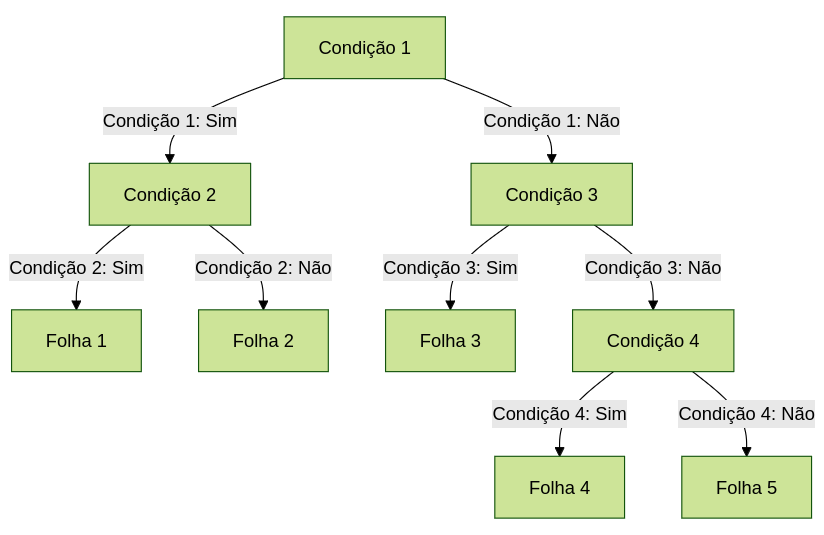
\includegraphics[keepaspectratio]{includes/mermaid-tree.png}}

}

\caption{\label{fig-arvore}Exemplo de estrutura de árvore de regressão.
A árvore tem cinco folhas e quatro nós internos.}

\end{figure}%

\vspace{12pt}

O espaço dos preditores é dividido em \(J\) regiões distintas e
disjuntas denotadas por \(R_1, R_2, \dots, R_J\). Essas regiões são
construídas em formato de caixa de forma a minimizar a soma dos
quadrados dos resíduos. Dessa forma, pode-se modelar a variável resposta
como uma constante \(c_j\) em cada região \(R_j\):

\[
f\left(x\right) = \sum^J_{j=1}c_j I\left(x \in R_j \right)\text{.}
\]

O estimador para a constante \(c_j\) é encontrado pelo método de mínimos
quadrados. Assim, deve-se minimizar
\(\sum_{x_i \in R_j} \left[y_i - f\left(x_i\right)\right]^2\). No
entanto, perceba que \(f\left(x_i\right)\) está sendo avaliado somente
em um ponto específico \(x_i\), o que reduzirá \(f\left(x_i\right)\)
para uma constante \(c_j\). É fácil de se chegar ao resultado se for
observada a definição da função indicadora \(I\left(x \in R_j\right)\):

\[
I_{R_j}(x_i) =
\begin{cases}
    1,& \text{se } x_i \in R_j \\
    0,& \text{se } x_i \notin R_j
\end{cases}\text{.}
\]

Como as regiões são disjuntas, \(x_i\) não pode estar simultaneamente em
duas regiões. Assim, para um ponto específico \(x_i\), apenas um dos
casos da função indicadora será diferente de 0. Portanto,
\(f\left(x_i\right) = c_j\). Agora, derivando
\(\sum_{x_i \in R_j}\left(y_i - c_j\right)^2\) em relação a \(c_j\)

\begin{equation}\phantomsection\label{eq-partialdev}{
\frac{\partial}{\partial{c_j}}\sum_{x_i \in R_j} \left(y_i - c_j\right)^2 = -2\sum_{x_i \in R_j} \left(y_i - c_j\right)
}\end{equation} e, ao igualar a Equação~\ref{eq-partialdev} a 0, tem-se
a seguinte igualdade:

\[
\sum_{x_i \in R_j} \left(y_i - \hat{c}_j\right) = 0\text{.}
\]

Expandindo o somatório e dividindo pelo número total de pontos \(N_j\)
na região \(R_j\), concluí-se que o estimador de \(c_j\), denotado por
\(\hat{c}_j\), é simplesmente a média dos valores observados \(y_i\) na
região \(R_j\):

\begin{equation}\phantomsection\label{eq-estimacjdev}{
\sum_{x_i \in R_j} y_i - \hat{c}_j N_j = 0 \Rightarrow \hat{c}_j = \frac{1}{N_{j}}\sum_{x_i \in R_j} y_i\text{.}
}\end{equation}

\vspace{12pt}

No entanto, JAMES et al. (2013) caracteriza como inviável considerar
todas as possíveis partições do espaço das variáveis independentes em
\(J\) caixas devido ao alto custo computacional. Dessa forma, a
abordagem a ser adotada é uma divisão binária recursiva. O processo
começa no topo da árvore, o ponto em que contém todas as observações, e
continua sucessivamente dividindo o espaço dos preditores. As divisões
são indicadas como dois novos ramos na árvore, como pode ser visto na
Figura~\ref{fig-arvore}.

\vspace{12pt}

Para executar a divisão binária recursiva, deve-se primeiramente
selecionar a variável independente \(X_j\) e o ponto de corte \(s\) tal
que a divisão do espaço dos preditores conduza a maior redução possível
na soma dos quadrados dos resíduos. Dessa forma, definimos dois
semi-planos:

\[
R_{1}\left(j, s\right) = \{X | X_j \leq s\} \text{ e } R_{2}\left(j, s\right) = \{X | X_j > s\}\text{,}
\] e procuramos a divisão da variável \(j\) e o ponto de corte \(s\) que
minimizem a seguinte expressão:

\[
\min_{j, s}\left[\min_{c_1} \sum_{x_i \in R_1\left(j, s\right)} \left(y_i - c_{1}\right)^2 + \min_{c_2} \sum_{x_i \in R_2\left(j, s\right)} \left(y_i - c_{2}\right)^2\right]\text{,}
\] em que \(c_1\) e \(c_2\) é a média da variável dependente para as
observações nas regiões \(R_1\left(j, s\right)\) e
\(R_2\left(j, s\right)\), respectivamente. Após determinar a melhor
divisão, os dados são particionados nessas duas regiões, e o processo é
repetido recursivamente para todas as sub-regiões resultantes.

\vspace{12pt}

O tamanho da árvore pode ser considerado um hiperparâmetro para regular
a complexidade do modelo, pois uma árvore muito grande pode causar
sobreajuste aos dados de treinamento, capturando não apenas os padrões
relevantes, mas também o ruído. Como resultado, o modelo pode apresentar
bom desempenho nos dados de treinamento, mas falhar ao lidar com novos
dados devido à sua incapacidade de generalização. Por outro lado, uma
árvore muito pequena pode não captar padrões, relações e estruturas
importantes presentes nos dados. Dessa forma, a estratégia adotada para
selecionar o tamanho da árvore consiste em crescer uma grande árvore
\(T_0\), interrompendo o processo de divisão apenas ao atingir um
tamanho mínimo de observações nos nós. Posteriormente, a árvore \(T_0\)
é podada utilizando o critério de custo de complexidade, que será
definido a seguir.

\vspace{12pt}

Para o processo de poda da árvore, definimos uma árvore qualquer \(T\)
que pode ser obtida através do processo da poda de \(T_0\), de modo que
\(T \subset T_0\). Assim, sendo \(N_j\) a quantidade de pontos na região
\(R_j\), seja

\[
Q_j\left(T\right) = \frac{1}{N_j} \sum_{x_i \in R_j}\left(y_i - \hat{c}_j\right)^2
\] uma medida de impureza do nó pelo erro quadrático médio. Assim,
define-se o critério de custo de complexidade:

\[
C_{\alpha}\left(T\right) = \sum_{j = 1}^{|T|}N_jQ_j\left(T\right) + \alpha |T|\text{,}
\] em que \(|T|\) denota a quantidade total de folhas, e
\(\alpha \geq 0\) é um hiperparâmetro que equilibra o tamanho da árvore
e a adequação aos dados. A ideia é encontrar, para cada \(\alpha\), a
árvore \(T_{\alpha} \subset T_0\) que minimiza
\(C_{\alpha}\left(T\right)\). Valores grandes de \(\alpha\) resultam em
árvores menores, enquanto valores menores resultam em árvores maiores, e
\(\alpha = 0\) resulta na própria árvore \(T_0\). A busca por
\(T_{\alpha}\) envolve colapsar sucessivamente o nó interno que provoca
o menor aumento em \(\sum_j N_j Q_j\left(T\right)\), continuando o
processo até produzir uma árvore com um único nó. Esse processo gera uma
sequência de subárvores, dentre as quais existe, para cada valor de
\(\alpha\), uma única subárvore que minimiza
\(C_{\alpha}\left(T\right)\).

\vspace{12pt}

A estimação de \(\alpha\) pode ser realizada por validação cruzada com
cinco ou dez folds. Assim, a árvore final será \(T_{\hat \alpha}\). O
 Algoritmo~\ref{algo-buildtree}  exemplifica o processo de crescimento
de uma árvore de regressão:

\begin{algo}

\centering{

\begin{algorithm}[H]
\caption{Algoritmo para crescer uma árvore de regressão.}
\begin{algorithmic}
\State \textbf{1.} Use a divisão binária recursiva para crescer uma árvore grande $T_0$ nos dados de treinamento, parando apenas quando cada folha tiver menos do que um número mínimo de observações.

\vspace{3.7pt}

\State \textbf{2.} Aplique o critério de custo de complexidade à árvore grande \( T_0 \) para obter uma sequência de melhores subárvores \( T_\alpha \), em função de \( \alpha \).

\vspace{3.7pt}

\State \textbf{3.} Use validação cruzada $K\text{-Fold}$ para escolher \( \alpha \). Isto é, divida as observações de treinamento em $K$ folds. Para cada \( k = 1, \ldots, K \):
    \State \hspace{1em} (a) Repita os Passos 1 e 2 em todos os folds, exceto no $k\text{-ésimo}$ fold dos dados de
    \State \hspace{1em} treinamento.
    \State \hspace{1em} (b) Avalie o erro quadrático médio da estimação no $k\text{-ésimo}$ fold deixado
    \State \hspace{1em} de fora, em função de \( \alpha \).

    \vspace{3pt}

    \State \hspace{1em} Faça a média dos resultados para cada valor de \( \alpha \) e escolha \( \alpha \) que minimize o erro
    \State \hspace{1em} médio.

\vspace{3.7pt}

\State \textbf{4.} Retorne a subárvore \( T_{\hat{\alpha}} \) do Passo 2 que corresponde ao valor estimado de \( \alpha \).
\end{algorithmic}
\end{algorithm}

}

\caption{\label{algo-buildtree}Fonte: JAMES et al. (2013, p. 337).}

\end{algo}%

\vspace{12pt}

No caso de uma árvore de decisão para classificação, a principal
diferença está no critério de divisão dos nós e na poda da árvore. Para
a classificação, a predição em um nó \(j\), correspondente a uma região
\(R_j\) com \(N_j\) observações, será simplesmente a classe majoritária.
Assim, tem-se:

\[
\hat{p}_{jk} = \frac{1}{N_j}\sum_{x_i \in R_j} I\left(y_i = k\right)\text{,}
\] como sendo a proporção de observações da classe \(k\) no nó \(j\).
Dessa forma, as observações no nó \(j\) são classificadas na classe
\(k\left(j\right) = \arg \max_{k} \hat{p}_{jk}\), correspondente à
classe majoritária nesse nó.

\vspace{12pt}

Para a divisão dos nós no caso da regressão, foi utilizado o erro
quadrático médio como medida de impureza. Para a classificação, algumas
medidas comuns para \(Q_j\left(T\right)\) são o erro de classificação, o
índice de Gini ou a entropia cruzada.

\section{Métodos Ensemble}\label{muxe9todos-ensemble}

~~~As árvores de decisão são conhecidas por sua alta interpretabilidade,
mas geralmente apresentam um desempenho preditivo inferior em comparação
com outros modelos e algoritmos. No entanto, é possível superar essa
limitação construindo um modelo preditivo que combina a força de uma
coleção de estimadores base, um processo conhecido como aprendizado em
conjunto (Ensemble Learning). De acordo com HASTIE et al. (2009), o
aprendizado em conjunto pode ser dividido em duas etapas principais: a
primeira etapa consiste em desenvolver uma população de algoritmos de
aprendizado base a partir dos dados de treinamento, e a segunda etapa
envolve a combinação desses algoritmos para formar um estimador
agregado. Portanto, nesta seção, serão definidos os métodos de
aprendizado em conjunto utilizados neste trabalho.

\subsection{Bagging}\label{bagging}

~~~O algoritmo de Bootstrap Aggregation, ou Bagging, foi introduzido por
BREIMAN (1996). Sua ideia principal é gerar um estimador agregado a
partir de múltiplas versões de um preditor, que são criadas por meio de
amostras bootstrap do conjunto de treinamento, utilizadas como novos
conjuntos de treinamento. O Bagging pode ser empregado para melhorar a
estabilidade e a predição de modelos ou algoritmos de aprendizado de
máquina, além de reduzir a variância e evitar o sobreajuste. Por
exemplo, o Bagging pode ser utilizado para melhorar o desempenho da
árvore de regressão descrita anteriormente.

\vspace{12pt}

BREIMAN (1996) define formalmente o algoritmo de Bagging, que utiliza um
conjunto de treinamento \(\mathcal{L}\). A partir desse conjunto, são
geradas amostras bootstrap \(\mathcal{L}^{(B)}\) com \(B\) réplicas,
formando uma coleção de modelos \(\{f(x, \mathcal{L}^{(B)})\}\), onde
\(f\) representa um modelo estatístico ou algoritmo treinado nas
amostras bootstrap para prever ou classificar uma variável dependente
\(y\) com base em variáveis independentes. Se a variável dependente
\(y\) for numérica, a predição é obtida pela média das estimações dos
modelos:

\[
f_{B}\left(x\right) = \frac{1}{B} \sum_{b = 1}^B f \left(x, \mathcal{L}^{\left(B\right)}\right)\text{,}
\] em que \(f_{B}\) representa a predição agregada. No caso em que \(y\)
prediz uma classe, utiliza-se a votação majoritária. Ou seja, se
estivermos classificando em classes \(j \in \{1, \dots, J\}\), então
\(N_j = \#\{B; f(x, \mathcal{L}^{(B)}) = j\}\) representa o número de
vezes que a classe \(j\) foi predita pelos estimadores. Assim:

\[
f_{B}\left(x\right) = \arg \max_{j} N_j\text{.}
\] isto é, o \(j\) para o qual \(N_j\) é máximo

\vspace{12pt}

Embora a técnica de Bagging possa melhorar o desempenho de uma árvore de
regressão ou de classificação, isso geralmente vem ao custo de menor
interpretabilidade. Quando o Bagging é aplicado a uma árvore de
regressão, construímos \(B\) árvores de regressão usando \(B\) réplicas
de amostras bootstrap e tomamos a média das predições resultantes (JAMES
et al., 2013). Nesse processo, as árvores de regressão crescem até seu
máximo, sem passar pelo processo de poda, resultando em cada árvore
individual com alta variância e baixo viés. No entanto, ao agregar as
predições das \(B\) árvores, a variância é reduzida.

\vspace{12pt}

Para mitigar a falta de interpretabilidade do método Bagging aplicado a
árvores de regressão, pode-se utilizar a medida de impureza baseada no
erro quadrático médio como uma métrica para avaliar a importância das
variáveis independentes. Um valor elevado na redução total média do erro
quadrático médio, calculado com base nas divisões realizadas por um
determinado preditor em todas as \(B\) árvores, indica que o preditor é
importante.

\vspace{12pt}

As árvores construídas pelo algoritmo de árvore de decisão se beneficiam
da estratégia de agregação do Bagging, principalmente por meio da
redução da variância das previsões. No entanto, esse benefício é
limitado pela correlação existente entre as árvores geradas. Se essas
árvores forem variáveis aleatórias independentes e identicamente
distribuídas (i.i.d.), cada uma com variância \(\sigma^2\), a variância
da média das previsões das \(B\) árvores será \(\frac{1}{B} \sigma^2\).

\vspace{12pt}

Contudo, se as árvores forem apenas identicamente distribuídas (i.d.),
mas não independentes, apresentando uma correlação positiva \(\rho\), a
variância da média das previsões passa a ser dada por:

\begin{equation}\phantomsection\label{eq-cor}{
\rho \sigma^2 + \frac{1 - \rho}{B}\sigma^2\text{.}
}\end{equation}

Nesse caso, à medida que o número de árvores \(B\) tende ao infinito, o
segundo termo da expressão se aproxima de zero, mas o primeiro termo
permanece constante. Isso demonstra que os ganhos proporcionados pelo
Bagging são limitados pela correlação entre as árvores (HASTIE et al.,
2009).

\vspace{12pt}

Essa correlação ocorre porque as árvores geradas pelo Bagging tendem a
ser bastante semelhantes. As variáveis selecionadas para as divisões são
escolhidas com base na maior redução do erro nas regiões, e,
frequentemente, as mesmas variáveis são as que mais contribuem para essa
redução, sendo repetidamente escolhidas. Uma forma de reduzir essa
correlação - e, com isso, melhorar o desempenho do Bagging - é por meio
do algoritmo Random Forest, que será apresentado a seguir.

\subsection{Random Forest}\label{random-forest}

\begin{algo}

\centering{

\begin{algorithm}[H]
\caption{Algoritmo de uma Random Forest para regressão ou classificação.}
\begin{algorithmic}
\State \hspace{1em} \textbf{1.} Para b = 1 até B:

\vspace{0.8em}

    \State \hspace{2em} (a) Construa amostras bootstrap $\mathbf{\mathcal{L}}^*$ de tamanho \( N \) dos dados de
    \State \hspace{3.6em} \vspace{0.1em} treinamento.

    \State \hspace{2em} (b) Faça crescer uma árvore de floresta aleatória \( T_b \) para os dados bootstrap,
    \State \hspace{3.6em} repetindo recursivamente os seguintes passos para cada folha da árvore,
    \State \hspace{3.6em} \vspace{0.5em} até que o tamanho mínimo do nó \( n_{min} \) seja atingido:
    \State \hspace{4em} \vspace{0.1em} i. Selecione \( m \) variáveis aleatoriamente entre as \( p \) variáveis.
    \State \hspace{4em} \vspace{0.1em} ii. Escolha a melhor variável para divisão entre as \( m \).
    \State \hspace{4em} \vspace{0.1em} iii. Divida o nó em dois subnós.

\vspace{0.8em}

\State \hspace{1em} \textbf{2.} Por fim, o conjunto de árvores \( \{T_b\}^{B}_1\) é construído.

\vspace{1em}

\State \hspace{0.7em} No caso da regressão, para fazer uma predição em um novo ponto \( x \), temos a seguinte função:


$$
\hat{f}^{B}_{rf}\left(x\right) = \frac{1}{B}\sum^{B}_{b = 1} T_{b}\left(x\right)
$$

\vspace{1em}

\State \hspace{0.7em} Para a classificação é utilizado o voto majoritário. Assim, seja $\hat{C}_{b}\left(x\right)$ a predição da classe da árvore de floresta aleatória $b$. Assim:

$$
\hat{C}^{B}_{rf}\left(x\right) = \arg \max_c \sum^{B}_{b = 1}I\left(\hat{C}_b\left(x\right) = c\right)\text{,}
$$

\State em que $c$ representa as classes possíveis.

\end{algorithmic}
\end{algorithm}

}

\caption{\label{algo-rf}Fonte: HASTIE et al. (2009, p. 588).}

\end{algo}%

~~~O algoritmo Random Forest é uma técnica derivada do método Bagging,
mas com modificações específicas na construção das árvores. O objetivo é
reduzir a variância ao diminuir a correlação entre as árvores, sem
aumentar significativamente a variabilidade. Isso é alcançado durante o
processo de crescimento das árvores por meio da seleção aleatória de um
subconjunto de variáveis independentes antes de cada divisão.

\vspace{12pt}

No algoritmo Random Forest, ao construir uma árvore a partir de amostras
bootstrap, selecionam-se aleatoriamente \(m \leq p\) das \(p\) variáveis
independentes como candidatas para a divisão (sendo \(m = p\) no caso do
Bagging). Assim, diferentemente do Bagging, o Random Forest não
considera todas as \(p\) variáveis ao escolher a divisão que minimiza o
erro das regiões, mas apenas uma amostra aleatória de \(m\) variáveis.

\vspace{12pt}

Essa seleção aleatória de variáveis independentes ajuda a resolver um
dos principais problemas do Bagging, a tendência de gerar árvores muito
semelhantes, resultando em previsões altamente correlacionadas. O Random
Forest mitiga esse problema ao criar oportunidades para que diferentes
preditores sejam considerados em cada divisão. Em média, uma fração
\((p - m)/p\) das divisões sequer incluirá o preditor mais forte como
candidato, o que aumenta a chance de seleção de outros preditores (JAMES
et al., 2013). Esse mecanismo reduz a correlação entre as árvores,
contribuindo para uma menor variabilidade nas previsões agregadas.

\vspace{12pt}

A quantidade de variáveis independentes \(m\) selecionadas
aleatoriamente é um hiperparâmetro que pode ser estimado por meio de
validação cruzada. Valores comumente utilizados são \(m = \sqrt{p}\) com
quantidade mínima de observações no nó igual a um, no caso de
classificação, e \(m = p/3\) com quantidade mínima de observações no nó
igual a cinco, no caso de regressão (HASTIE et al., 2009).

\vspace{12pt}

Quando o número total de variáveis é grande, mas apenas algumas são
realmente relevantes, o Random Forest pode apresentar desempenho
inferior com valores muito pequenos de \(m\), pois isso reduz a
probabilidade de que as variáveis mais importantes sejam selecionadas.
Por outro lado, utilizar um valor pequeno de \(m\) pode ser vantajoso
quando há muitos preditores altamente correlacionados. Além disso, assim
como no Bagging, o Random Forest não sofre de sobreajuste com o aumento
do número de árvores \(B\). Dessa forma, é suficiente utilizar um valor
de \(B\) grande o bastante para que a taxa de erro se estabilize (JAMES
et al., 2013).

\subsection{Boosting Trees}\label{boosting-trees}

~~~O Boosting, assim como o Bagging, é um método destinado a melhorar o
desempenho de modelos ou algoritmos. No entanto, neste trabalho, o
Boosting foi aplicado apenas às árvores de regressão. Portanto, a
explicação do Boosting será restrita ao caso de Boosting Trees. Seu
algoritmo pode ser observado no  Algoritmo~\ref{algo-boos} .

\vspace{12pt}

\begin{algo}

\centering{

\begin{algorithm}[H]
\caption{Método Boosting aplicado a árvores de regressão.}
\begin{algorithmic}
\State \hspace{1em} \textbf{1.} Defina $\hat{f}\left(x\right) = 0 \text{ e } r_i = y_i$ para todos os $i$ no conjunto de treinamento

\vspace{0.8em}

\State \hspace{1em} \vspace{0.8em} \textbf{2.} Para $b = 1, 2, \dots, B$, repita:

  \State \hspace{2em} (a) Ajuste uma árvore $\hat{f}^b$ com $d$ divisões para os dados de treinamento $\left(X, r\right)$.

  \State \hspace{2em} (b) Atualize $\hat{f}$ adicionando uma versão com o hiperparâmetro $\lambda$ de taxa de
  \State \hspace{3.6em} aprendizado:

$$
\hat{f}\left(x\right) \gets \hat{f}\left(x\right) + \lambda \hat{f}^b\left(x\right)
$$

  \vspace{0.1em}

  \State \hspace{2em} (c) Atualize os resíduos,

$$
r_i \gets r_i - \lambda \hat{f}^b\left(x_{i}\right)
$$

\vspace{1em}

\State \hspace{1em} \textbf{3.} Retorne o modelo de boosting,

$$
\hat{f}\left(x\right) = \sum_{b = 1}^B \lambda \hat{f}^b\left(x\right)
$$


\end{algorithmic}
\end{algorithm}

}

\caption{\label{algo-boos}Fonte: JAMES et al. (2013, p. 349).}

\end{algo}%

No algoritmo de Bagging, cada árvore é construída e ajustada utilizando
amostras bootstrap, e ao final, um estimador agregado
\(\varphi_B\)\hspace{0pt} é formado a partir das \(B\) árvores. O
Boosting Trees funciona de maneira semelhante, mas sem o uso de amostras
bootstrap. A ideia central do Boosting é corrigir os erros das árvores
anteriores, ajustando as novas árvores aos resíduos gerados pelas
predições anteriores. Assim, as árvores no Boosting são construídas de
forma sequencial, incorporando gradualmente as informações dos erros
cometidos pelas árvores anteriores.

\vspace{12pt}

No caso da regressão, o Boosting combina um grande número de árvores de
decisão \(\hat{f}^1, \dots, \hat{f}^B\). A primeira árvore é construída
utilizando o conjunto de dados original, e seus resíduos são calculados.
Com a primeira árvore ajustada, a segunda árvore é ajustada aos resíduos
da árvore anterior e, em seguida, é adicionada ao estimador para
atualizar os resíduos. Dessa forma, os resíduos servem como informação
crucial para construir novas árvores e corrigir os erros das árvores
anteriores. Como cada nova árvore depende das árvores já construídas,
árvores menores são suficientes (JAMES et al., 2013).

\vspace{12pt}

O processo de aprendizado do Boosting é mais lento, o que geralmente
resulta em modelos mais precisos, embora mais custosos
computacionalmente. Esse processo de aprendizado pode ser controlado por
um hiperparâmetro \(\lambda\) chamado de shrinkage, ou taxa de
aprendizado, permitindo que mais árvores, com formas diferentes,
corrijam os erros das árvores passadas. No entanto, um valor muito
pequeno para \(\lambda\) requer uma quantidade muito maior \(B\) de
árvores e, diferente do Bagging e Random Forest, o Boosting pode sofrer
de sobreajuste se a quantidade de árvores é muito grande. Além disso, a
quantidade de divisões \(d\) em cada árvore, que controla a complexidade
do boosting, pode ser considerada também um hiperparâmetro. Para
\(d = 1\), ajusta-se um modelo aditivo, pois cada árvore contém apenas
um nó.

\subsection{Stacked generalization}\label{sec-stacking_cite}

~~~O Stacked Generalization, ou Stacking, é um método de ensemble que
consiste em treinar um modelo gerado a partir da combinação da predição
de vários outros modelos, visando melhorar a precisão das predições.
Esse método pode ser aplicado a qualquer modelo estatístico ou algoritmo
de aprendizado de máquina. A ideia principal é atribuir pesos às
predições, de modo a dar maior importância aos modelos que produzem
melhores resultados, ao mesmo tempo em que se evita atribuir altos pesos
a modelos com alta complexidade.

\vspace{12pt}

Matematicamente, o Stacking define predições
\(\hat{f}_m^{-i}\left(x\right)\) em \(x\), utilizando o modelo \(m\),
aplicado ao conjunto de treinamento com a \(i\text{-ésima}\) observação
dos dados de treinamento removida (HASTIE et al., 2009). Os pesos dos
modelos são estimados por meio de uma regressão linear de mínimos
quadrados, ajustando \(y_i\) em relação a
\(\hat{f}^{-i}\left(x\right)\), para \(m=1,\dots,M\). A estimativa dos
pesos é obtida pela seguinte expressão:

\[
\hat{w}^{st} = \arg \min_{w} \sum^{N}_{i = 1} \left[y_i - \sum^{M}_{m = 1} w_m \hat{f}^{-i}_m\left(x_i\right)\right]^2\text{.}
\]

A estimação final é \(\sum_{m} \hat{w}_m^{st} \hat{f}_m\left(x\right)\).
Assim, em vez de escolher um único modelo, o método de Stacking combina
os modelos utilizando pesos estimados, o que melhora a performance
preditiva, mas pode comprometer a interpretabilidade. Além disso, ao
utilizar validação cruzada baseada no método leave-one-out para as
predições \(\hat{f}^{-i}_{m}\left(x\right)\), o Stacking evita atribuir
pesos excessivos a modelos de alta complexidade, reduzindo o risco de
sobreajuste.

\subsection{Gradient Boosting}\label{gradient-boosting}

~~~O algoritmo de Gradient Boosting é semelhante ao Boosting. Ele
constrói modelos aditivos ajustando sequencialmente funções base aos
pseudos-resíduos em cada iteração, que, por sua vez, correspondem a
direção contrária dos gradientes da função de perda (FRIEDMAN, 2002).
Esses pseudos-resíduos indicam a direção na qual a função de perda está
sendo minimizada, orientando o ajuste dos modelos seguintes.

\vspace{12pt}

Neste trabalho, foram utilizadas diferentes implementações do Gradient
Boosting. Todas elas, no entanto, empregam o método com árvores de
regressão como funções base, variando apenas em aspectos como a
construção das árvores ou otimizações voltadas à eficiência
computacional. Sendo assim, o algoritmo apresentado a seguir corresponde
ao Gradient Tree Boosting, cuja formulação é detalhada no
 Algoritmo~\ref{algo-gradboos} .

\begin{algo}

\centering{

\begin{algorithm}[H]
\caption{Algoritmo de Gradient Tree Boosting.}
\begin{algorithmic}
\State \hspace{1em} \textbf{1.} Inicialize $f_0\left(x\right) = \arg \min_{\gamma} \sum_{i = 1}^N L\left(y_i, \gamma \right)$

\vspace{0.8em}

\State \hspace{1em} \vspace{0.8em} \textbf{2.} Para $m = 1$ até $M$:

  \State \hspace{2em} (a) Para $i = 1, 2, \dots, N$, calcule

$$
{r}_{im} = -\left[\frac{\partial L\left(y_i, f\left(x_i \right)\right)}{\partial f\left(x_i\right)}\right]_{f = f_{m - 1}}
$$

  \State \hspace{2em} (b) Ajuste uma árvore de regressão aos pseudo-resíduos $r_{im}$, obtendo regiões
  \State \hspace{3.6em} terminais $R_{jm}, \ j = 1, 2, \dots, J_m$.


  \State \vspace{0.1em}

  \State \hspace{2em} (c) Para $j = 1, 2, \dots, J_m$, calcule

$$
\gamma_{jm} = \arg \min_{\gamma} \sum_{x_i \in R_{jm}} L\left(y_i, f_{m - 1}\left(x_i\right) + \gamma\right)
$$

  \vspace{0.1em}

  \State \hspace{2em} (d) Atualize $f_m\left(x\right) = f_{m - 1}\left(x\right) + \lambda \sum^{J_m}_{j = 1} \gamma_{jm} I\left(x \in R_{jm}\right)$

\vspace{1em}

\State \hspace{1em} \textbf{3.} Retorne $\hat{f}\left(x\right) = f_M\left(x\right)$

\end{algorithmic}
\end{algorithm}

}

\caption{\label{algo-gradboos}Fonte: HASTIE et al. (2009, p. 361).}

\end{algo}%

\vspace{12pt}

O Gradient Boosting aplicado para árvores de regressão, tem que cada
função base é uma árvore de regressão com \(J_m\) folhas. Dessa forma,
cada árvore de regressão tem a seguinte forma aditiva:

\begin{equation}\phantomsection\label{eq-treebost}{
h\left(x;\{R_{jm}\}^{J_{m}}_{1}\right) = \sum^{J_m}_{j = 1} b_{jm} I\left(x \in R_{jm}\right)\text{,}
}\end{equation} em que \(\{R_{jm}\}^{J_m}_{1}\) representa as regiões
disjuntas que, em conjunto, cobrem o espaço das variáveis preditoras.
Essas regiões correspondem às folhas da respectiva árvore de regressão.

\vspace{12pt}

Como as regiões são disjuntas, a partir da Equação~\ref{eq-treebost}, a
estimativa de \(b_{jm}\) - a predição associada à região
\(R_{jm}\)\hspace{0pt} - será simplesmente a média dos pseudo-resíduos
\(r_{im}\):

\[
\hat{b}_{jm} = \frac{1}{N_{jm}} \sum_{x_i \in R_{jm}} r_{im}\text{,}
\] onde \(N_{jm}\) denota o número de observações na região \(R_{jm}\).
Os pseudo-resíduos \(r_{im}\)\hspace{0pt} representam a direção
contrária dos gradientes da função perda \(L\), conforme expressos na
linha 2(a) do  Algoritmo~\ref{algo-gradboos} , e indicam a direção de
minimização de \(L\).

\vspace{12pt}

Assim, cada árvore de regressão é ajustada aos novos pseudo-resíduos,
com o objetivo de minimizar o erro das árvores anteriores. O estimador
é, então, atualizado separadamente em cada região
\(R_{jm}\)\hspace{0pt}, conforme descrito a seguir:

\[
f_m\left(x\right) = f_{m - 1}\left(x\right) + \lambda \sum^{J_m}_{j = 1} \gamma_{jm} I\left(x \in R_{jm}\right)\text{,}
\] em que
\(\gamma_{jm} = \arg \min_{\gamma} \sum_{x_i \in R_{jm}} L\left(y_i, f_{m - 1}\left(x_i\right) + \gamma\right)\)
representa uma constante ótima para cada região. O parâmetro
\(\lambda\), assim como no algoritmo de boosting, é o hiperparâmetro de
shrinkage, utilizado para controlar a taxa de aprendizado. Valores
menores de \(\lambda\) exigem um número maior de iterações \(M\).

\vspace{12pt}

As outras implementações de Gradient Boosting aplicadas a árvores de
decisão tem seus próprios motivos de existência. Esses motivos incluem a
busca por maior eficiência computacional, adição de recursos e até mesmo
maior flexibilidade. As duas outras implementações utilizadas foram o
Extreme Gradient Boosting (XGBoost) e Light Gradient Boosting
(LightGBM).

\vspace{12pt}

O Extreme Gradient Boosting é uma implementação altamente eficiente e
flexível do algoritmo de Gradient Boosting aplicado a árvores de
decisão. Um de seus principais diferenciais é a incorporação de técnicas
de regularização, que ajudam a reduzir o sobreajuste e a melhorar a
generalização do modelo.

\vspace{12pt}

A regularização é feita por meio de um termo adicional que penaliza a
complexidade das árvores, definido como:

\[
\Omega\left(f\right) = \gamma T + \frac{1}{2}\lambda\|\omega\|^{2}\text{,}
\] em que \(T\) é a quantidade de folhas na árvore, \(\|\omega\|^{2}\) é
a soma do quadrado dos pesos associados às folhas. \(\gamma\) e
\(\lambda\) são os parâmetros de regularização, em que \(\lambda\)
penaliza os pesos das folhas e \(\gamma\) penaliza a quantidade de
folhas nas árvores. As implementações do Extreme Gradient Boosting em
\textbf{Python}, por padrão, utilizam a regularização L2, mas também
permitem a aplicação da regularização L1.

\vspace{12pt}

Assim como o XGBoost, as implementações existentes do LightGBM também
permitem o uso de regularização L1 ou L2, embora nenhuma das
implementações a utilize por padrão. O LightGBM tem como foco a alta
velocidade de treinamento e a eficiência no uso da memória, graças ao
algoritmo baseado em histogramas (Histogram-Based Algorithm). Nesse
método, os valores contínuos das variáveis são agrupados em intervalos
discretos - como em um histograma - o que evita a avaliação de cada
ponto individualmente durante as divisões das árvores, reduzindo
significativamente o custo computacional.

\chapter{Metodologia}\label{metodologia}

\section{Obtenção dos dados}\label{obtenuxe7uxe3o-dos-dados}

~~~Os dados foram obtidos em 2023 por meio de web scraping, que é uma
técnica para coletar dados de páginas da internet. Para isso, foram
utilizadas as linguagens de programação \textbf{R} e \textbf{Python}. No
\textbf{R}, os pacotes \href{https://xml2.r-lib.org/}{\textbf{xml2}} e
\href{https://rvest.tidyverse.org/}{\textbf{rvest}} foram utilizados
para extrair dados de páginas estáticas de forma estruturada. No
\textbf{Python}, as bibliotecas
\href{https://scrapy.org/}{\textbf{Scrapy}} e
\href{https://playwright.dev/python/}{\textbf{Playwright}}, desenvolvida
pela Microsoft, foram empregadas, sendo esta última essencial para a
interação com componentes dinâmicos da página, possibilitando a extração
de informações que exigem interações como cliques ou rolagem de página
para ser gerada. Além dessas ferramentas, foram implementadas técnicas
de rotacionamento de IPs e de modificação das informações do usuário que
acessa o site, a fim de evitar bloqueios durante o processo de coleta de
dados, garantindo assim a continuidade e eficácia da extração. A API
utilizada para gerenciar a rotação de informações dos usuários que
acessam o site foi desenvolvida pela empresa ScrapeOps.

\vspace{12pt}

Assim, utilizando as ferramentas e técnicas de web scraping, foram
coletadas as variáveis que poderiam fazer sentido para a modelagem,
priorizando aquelas com menor chance de gerar problemas durante o
tratamento dos dados, como, por exemplo, ter muitos valores ausentes. Ao
todo, foram extraídas 25 variáveis, das quais 11 são quantitativas e 14
qualitativas nominais, sendo 12 de caráter dicotômico. No entanto, nem
todas as variáveis foram obtidas diretamente por web scraping. As
coordenadas geográficas, latitude e longitude, por exemplo, foram
geradas por meio da geocodificação dos endereços de cada imóvel,
utilizando o pacote
\href{https://jessecambon.github.io/tidygeocoder/}{\textbf{tidygeocoder}}
da linguagem \textbf{R}. Dessa forma, foram consideradas as seguintes
variáveis, todas obtidas por meio de web scraping, com exceção das
coordenadas geográficas, que foram obtidas por geocodificação dos
endereços:

\begin{itemize}
\item
  Valor do imóvel: variável dependente que será modelada e constitui o
  principal foco de análise deste trabalho;
\item
  Valor médio do aluguel no bairro: média dos valores de aluguel
  anunciados para imóveis localizados no respectivo bairro. Os dados
  foram obtidos por meio de web scraping, e a média final foi calculada
  com base nos valores coletados nos anúncios da região;
\item
  Área média dos imóveis anunciados para aluguel no bairro: média das
  áreas, em \(m^2\), dos imóveis disponíveis para aluguel no respectivo
  bairro. Assim como os valores de aluguel, os dados de área de aluguel
  foram obtidos por meio de web scraping, sendo a média calculada a
  partir das áreas informadas nos anúncios coletados;
\item
  Área: área total do imóvel, medida em \(m^2\);
\item
  Condomínio: valor mensal pago pelo condomínio do imóvel;
\item
  IPTU: imposto cobrado sobre imóveis urbanos;
\item
  Banheiros: quantidade de banheiros disponíveis na propriedade;
\item
  Vagas de estacionamento: número total de vagas de estacionamento
  disponíveis;
\item
  Quartos: quantidade de quartos no imóvel;
\item
  Latitude: posição horizontal, medida em frações decimais de graus;
\item
  Longitude: posição vertical, também medida em frações decimais de
  graus, assim como a latitude;
\item
  Tipo do imóvel: seis categorias foram consideradas: apartamentos,
  casas, casas de condomínio, flats e terrenos de lotes comerciais e de
  condomínio;
\item
  Endereço: nome do endereço onde o imóvel está localizado;
\item
  Variáveis dicotômicas: indicam a presença (1) ou ausência (0) de
  determinadas características no imóvel, como área de serviço,
  academia, elevador, espaço gourmet, piscina, playground, portaria 24
  horas, quadra de esportes, salão de festas, sauna, spa e varanda
  gourmet.
\end{itemize}

\vspace{12pt}

No entanto, com base nas observações realizadas durante o estudo, nem
todas as variáveis coletadas foram utilizadas na modelagem do valor dos
imóveis. Algumas foram excluídas devido a uma quantidade excessiva de
valores ausentes, enquanto outras se mostraram pouco significativas para
explicar o valor do imóvel. No caso da variável de endereço, utilizada
para a obtenção das coordenadas por meio da geocodificação, muitos
registros apresentaram baixa precisão, frequentemente por não incluírem
o número do imóvel ou conterem apenas o nome da rua e do bairro. Isso
resultou em uma localização geográfica genérica, fazendo com que
diversos imóveis fossem posicionados de forma centralizada, como, por
exemplo, no meio da rua. Após o processo de coleta e limpeza dos dados,
o banco de dados final conta com 31.781 observações.

\vspace{12pt}

Além dos dados mencionados, foram também utilizados dados geográficos
sobre a cidade de João Pessoa, incluindo informações sobre ciclovias,
faixas exclusivas de ônibus, corredores de ônibus, área rural, bairros,
escolas públicas, parques, praças e rios. No entanto, esses dados foram
empregados exclusivamente na construção dos mapas na aplicação final. As
informações foram obtidas no site
\url{https://filipeia.joaopessoa.pb.gov.br/}. A localização das escolas
públicas foi obtida a partir do INEP (Instituto Nacional de Estudos e
Pesquisas Educacionais Anísio Teixeira).

\section{Análise exploratória de
dados}\label{anuxe1lise-exploratuxf3ria-de-dados}

~~~A análise exploratória de dados é uma das primeiras etapas de
qualquer estudo que utiliza a estatística como ferramenta principal,
pois permite identificar padrões de comportamento nos dados e descobrir
relações entre as variáveis estudadas. Assim, após a coleta e
organização dos dados, a primeira etapa deste estudo consistiu em uma
análise descritiva. Essa análise possibilitou identificar padrões entre
os diferentes tipos de imóveis e como essas características podem
influenciar o seu valor. Para evidenciar esses comportamentos, foram
criados gráficos e tabelas que permitiram caracterizar as relações entre
as variáveis independentes e a variável dependente.

\vspace{12pt}

Nesta etapa, também foi analisada a correlação entre as variáveis
independentes utilizadas no modelo, o que possibilitou a criação de
novas variáveis com base na interação entre aquelas que apresentavam
alguma relação. Para isso, utilizou-se a correlação de Spearman
(SPEARMAN, 1961).

\vspace{12pt}

A correlação de Spearman é bastante semelhante à correlação de Pearson
(COHEN et al., 2009). No entanto, diferencia-se por ser uma medida não
paramétrica de correlação entre os postos das variáveis. Assim, o
coeficiente de correlação de Spearman é definido como o coeficiente de
correlação de Pearson aplicado às variáveis classificadas em postos:

\[
r_{s} = \rho_{rg_{X}, rg_{Y}} = \frac{cov\left(rg_{X}, rg_{Y}\right)}{\sigma_{rg_X}\sigma_{rg_Y}} \text{,}
\] em que \(\rho\) representa o coeficiente de Pearson aplicado aos
postos das variáveis, \(cov\left(rg_{X}, rg_{Y}\right)\) é a covariância
entre os postos, e \(\sigma_{rg_X}\) e \(\sigma_{rg_Y}\) são os desvios
padrão das variáveis em postos.

\vspace{12pt}

Portanto, essa etapa resultou na criação de quatro variáveis: a
quantidade total de cômodos do imóvel, o produto entre as coordenadas
geográficas e o preço médio do aluguel no bairro, a razão entre o número
de quartos e a área do imóvel, e o produto entre o número de quartos do
imóvel e a área média do aluguel no bairro. No entanto, a inclusão
dessas variáveis não levou à remoção das variáveis originais utilizadas
em sua construção, pois sua exclusão resultou em uma piora no desempenho
do modelo, tendo sido observado uma diminuição na métrica de erro
quadrático médio.

\vspace{12pt}

Com um maior entendimento dos dados, o próximo passo foi a construção do
modelo, incluindo as transformações aplicadas, o método de imputação de
valores ausentes e o tratamento de variáveis nominais. A próxima seção
detalhará os métodos utilizados nesse processo.

\section{Construção do modelo}\label{construuxe7uxe3o-do-modelo}

~~~No conjunto de dados extraído, foram avaliados diferentes modelos
para a estimação do valor do imóvel. O valor do imóvel foi explicado por
variáveis consideradas relevantes para o estudo, como: preço médio do
aluguel no bairro, área, área média do aluguel no bairro, número de
banheiros, vagas de estacionamento, número de quartos, latitude,
longitude, tipo de imóvel, variáveis dicotômicas obtidas durante o
processo de extração e variáveis criadas posteriormente ao processo de
raspagem dos dados. As variáveis relacionadas ao valor do condomínio e
IPTU foram excluídas do modelo devido à alta quantidade de valores
ausentes.

\vspace{12pt}

Após a seleção das variáveis, o conjunto de dados foi dividido em
conjuntos de treino e teste para avaliar o desempenho dos modelos. A
divisão foi realizada de forma estratificada, utilizando a classe
\texttt{sklearn.model\_selection.StratifiedShuffleSplit}, da biblioteca
\href{https://scikit-learn.org/stable/}{\textbf{scikit-learn}}. Essa
classe permite dividir a base de dados de maneira aleatória, preservando
a proporção das classes definidas.

\vspace{12pt}

A estratificação foi baseada em intervalos criados a partir da variável
que representa o valor dos imóveis. Foram definidos cinco intervalos: o
primeiro abrange valores entre o mínimo de R\$ 43.914 e R\$ 200.000; o
segundo, entre R\$ 200.000 e R\$ 400.000; o terceiro, entre R\$ 400.000
e R\$ 600.000; o quarto, entre R\$ 600.000 e R\$ 800.000; e a quinta,
valores acima de R\$ 800.000 até o máximo de R\$ 7.000.000. Dessa forma,
20\% do conjunto de dados foi reservado para o teste, enquanto os 80\%
restantes foram utilizados para o treinamento do modelo.

\vspace{12pt}

Para a aplicação das ferramentas de modelagem, foram utilizadas as
bibliotecas
\href{https://scikit-learn.org/stable/}{\textbf{scikit-learn}},
\href{https://lightgbm.readthedocs.io/en/stable/}{\textbf{LightGBM}} e
\href{https://xgboost.readthedocs.io/en/stable/}{\textbf{XGBoost}}. As
duas últimas foram empregadas especificamente na modelagem, enquanto a
primeira também foi utilizada para criar pipelines de pré-processamento
de dados, que organizam etapas sequenciais de preparação necessárias
para o tratamento adequado dos dados. Assim, os quatro modelos aplicados
na predição do valor do imóvel foram: Random Forest, Gradient Boosting,
LightGBM e XGBoost. Por fim, foi implementado o algoritmo de Stacking.

\vspace{12pt}

A implementação do Stacking na biblioteca
\href{https://scikit-learn.org/stable/}{\textbf{scikit-learn}} permite o
uso de um modelo para estimar os pesos atribuídos às predições dos
modelos base, por meio do argumento \texttt{final\_estimator} da classe
\texttt{StackingRegressor}. Por padrão, esse argumento corresponde a um
modelo linear do tipo Ridge, que realiza a combinação de forma
regularizada. Quando o modelo final é linear, obtém-se a formulação
clássica do Stacking, conforme discutido na
Seção~\ref{sec-stacking_cite}. No entanto, é possível utilizar outros
algoritmos nessa etapa. Neste trabalho, optou-se pelo algoritmo Random
Forest como \texttt{final\_estimator}, em substituição ao Ridge, devido
ao melhor desempenho preditivo do algoritmo Stacking com o Random Forest
nessa função. Embora o Random Forest tenha sido utilizado para essa
etapa, ele também foi empregado como estimador base, juntamente com os
outros três algoritmos.

\subsection{Etapas de
pré-processamento}\label{etapas-de-pruxe9-processamento}

~~~Após a organização e limpeza dos dados, foram realizadas
transformações nas variáveis para aprimorar a capacidade preditiva dos
modelos em relação aos valores dos imóveis. Além disso, foi aplicado um
tratamento específico para lidar com valores ausentes em algumas
variáveis do conjunto de dados. Esse tratamento foi restrito às
variáveis com menos de 20\% de valores ausentes, incluindo as variáveis
de número de banheiros, quartos, vagas, valor médio do aluguel e área
média do aluguel. Por outro lado, as variáveis de condomínio e IPTU
apresentaram um elevado percentual de valores ausentes, com a variável
de condomínio tendo quase 60\% de observações ausentes e a variável IPTU
mais de 80\%. Devido a essa alta proporção de valores ausentes, essas
variáveis foram excluídas.

\vspace{12pt}

O método utilizado para a imputação de valores ausentes foi o algoritmo
k-nearest neighbors (KNN). Esse algoritmo estima os valores ausentes de
acordo com a seguinte fórmula:

\[
\hat{y} = \frac{1}{k}\sum_{x_i \in N_k\left(x\right)}y_i\text{,}
\] em que \(N_k(x)\) representa o conjunto de \(k\) vizinhos mais
próximos de \(x\), ou seja, os pontos \(x_i\) no conjunto de dados que
estão mais próximos de \(x\). Essa proximidade é geralmente medida pela
distância Euclidiana, que é a métrica padrão utilizada pela classe
\texttt{KNNImputer} da biblioteca
\href{https://scikit-learn.org/stable/}{\textbf{scikit-learn}} para
imputação de valores ausentes. No processo de imputação, foi utilizado
um total de 17 vizinhos, definido pelo argumento \texttt{n\_neighbors}
da classe \texttt{KNNImputer}.

\vspace{12pt}

A transformação logarítmica \(\log\left(1 + x\right)\) foi aplicada para
estabilizar a variância e tornar a distribuição dos regressores mais
simétrica. Embora essa transformação tenha sido utilizada na maioria das
variáveis numéricas, algumas exceções foram feitas. Em particular, a
variável que representa o produto entre as coordenadas geográficas e o
valor do aluguel foi transformada usando a técnica de Yeo-Johnson (YEO;
JOHNSON, 2000), que apresenta a vantagem de ser aplicável a dados que
incluem valores negativos e zero. Além disso, as variáveis referentes ao
preço e à área do aluguel não foram transformadas com
\(\log\left(1 + x\right)\). A decisão foi tomada com base nas métricas
de avaliação do modelo, que indicaram uma queda de desempenho do modelo
quando essas variáveis eram transformadas.

\vspace{12pt}

A transformação de Yeo-Johnson é definida da seguinte forma:

\[
\psi(\lambda, x) = \begin{cases}
    [(1 + x)^\lambda - 1] / \lambda  &  \lambda \neq 0, \; x \ge 0 \\
    \ln(1 + x)                       &  \lambda = 0, \; x \ge 0 \\
    [(1 - x)^{2 - \lambda} - 1] / (\lambda - 2) \quad & \lambda \neq 2, \; x < 0 \\
    -\ln(1 - x)                     &   \lambda = 2, \; x < 0
\end{cases} \text{,}
\] em que \(\lambda\) é estimado por máxima verossimilhança. Além disso,
percebe-se que a transformação \(\log(1 + x)\) é um caso particular da
transformação de Yeo-Johnson quando \(\lambda = 0\) e \(x \ge 0\).

\vspace{12pt}

Para as variáveis categóricas, utilizou-se a classe
\texttt{OneHotEncoder}, da biblioteca
\href{https://scikit-learn.org/stable/}{\textbf{scikit-learn}}, que
converte as categorias em variáveis dicotômicas, criando uma nova coluna
para cada categoria. Especificamente, a \texttt{OneHotEncoder} foi
aplicada à variável que representa o tipo de imóvel, transformando cada
categoria em uma variável binária.

\vspace{12pt}

Após a aplicação da transformação logarítmica e de Yeo-Johnson às
variáveis numéricas, essas variáveis também foram padronizadas
utilizando a classe \texttt{StandardScaler}, disponível no módulo
\texttt{preprocessing} da biblioteca
\href{https://scikit-learn.org/stable/}{\textbf{scikit-learn}}. As
únicas variáveis que não foram padronizadas é o valor médio de área e
aluguel no bairro, pelo mesmo motivo dado anteriormente. Essa classe
ajusta os dados para que fiquem na mesma escala, padronizando-os de
acordo com a fórmula:

\[
z = \frac{x - \mu}{\sigma}\text{,}
\] em que \(\mu\) representa a média e \(\sigma\) o desvio padrão. Essa
padronização é essencial para garantir que os modelos estatísticos e de
aprendizado de máquina tratem as variáveis em escalas consistentes.

\subsection{Validação cruzada}\label{sec-val_cruz}

~~~A técnica utilizada para otimizar e determinar os hiperparâmetros dos
modelos, além de servir para otimizar o hiperparâmetro de vizinhos mais
próximos para a imputação de valores ausentes, foi a validação cruzada.
A validação cruzada serve para estimar um erro de generalização médio da
seguinte forma
\(Err = E\left[L\left(Y, \hat{f}\left(X\right)\right)\right]\), em que
\(L\) é uma função perda e \(\hat f\) é um estimador. Existem diversar
técnicas de validação cruzada, a que foi utilizada nesse trabalho é a
validação cruzada K-Fold.

\vspace{12pt}

A validação cruzada K-Fold é uma técnica que utiliza parte dos dados
para ajustar o modelo e outra parte para testá-lo. Nessa abordagem, os
dados são divididos em \(K\) folds. Em cada iteração, um desses folds é
reservado para testar o modelo, enquanto os \(K−1\) folds restantes são
usados para treiná-lo. O modelo é ajustado nos \(K−1\) subconjuntos e
avaliado no subconjunto de teste, permitindo estimar o erro de predição.
Esse processo é repetido \(K\) vezes, alternando o subconjunto de teste
em cada rodada, e ao final, os \(K\) erros de predição são combinados. O
erro de predição estimado pela validação cruzada é dado por:

\[
CV\left(\hat f\right) = \frac{1}{N}\sum_{i = 1}^N L\left(y_i, \hat{f}^{-k\left(i\right)}\left(x_i\right)\right)\text{,}
\] em que \(N\) representa o número total de observações, \(L\) é a
função de perda, \(y_i\) é o valor observado, \(x_i\) é a entrada
correspondente, \(\hat{f}^{-k(i)}\) é o modelo ajustado sem o
\(k\)-ésimo fold ao qual a observação \(i\) pertence, e
\(k: \{1, \dots, N\} \mapsto \{1, \dots, K\}\) indica a partição à qual
a observação \(i\) foi alocada por meio de randomização.

\begin{figure}

\centering{

\pandocbounded{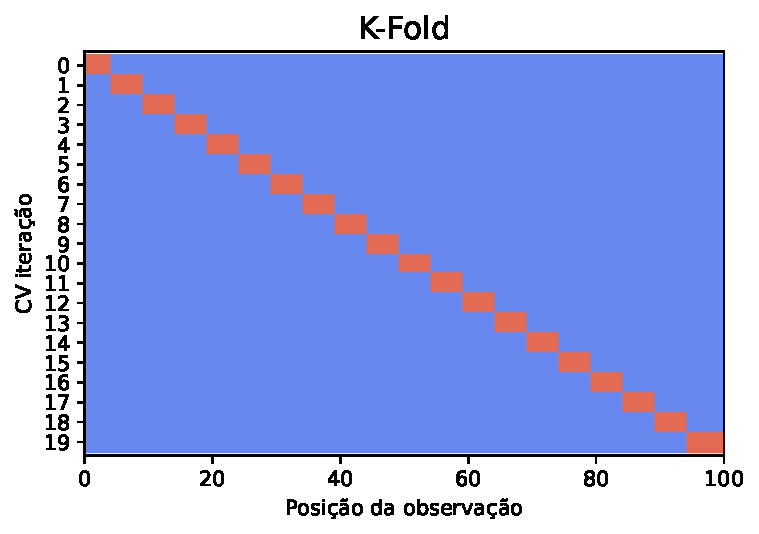
\includegraphics[keepaspectratio]{TCC_files/figure-pdf/fig-kfold-output-1.pdf}}

}

\caption{\label{fig-kfold}Visualização de K-Fold com 20 folds.}

\end{figure}%

\vspace{12pt}

A Figura~\ref{fig-kfold} ilustra exatamente o caso da validação cruzada
por K-Fold. As divisões do conjunto de dados para treinamento são
representados pela cor azul, enquanto as laranjas são os conjuntos de
validação, onde o modelo, após ser ajustado, será testado com uma função
perda \(L\).

\vspace{12pt}

Para realizar a validação cruzada com K-Fold nos modelos empregados
neste trabalho, utilizou-se uma função e uma classe da biblioteca
\href{https://scikit-learn.org/stable/}{\textbf{scikit-learn}}, ambas
disponíveis no módulo \texttt{model\_selection}. A função utilizada foi
a \texttt{cross\_val\_score}, que recebe o modelo por meio do argumento
\texttt{estimator}. A função perda para avaliação é especificado pelo
argumento \texttt{scoring}, enquanto a técnica de validação cruzada é
definida pelo argumento \texttt{cv}. Especificamente, foi empregada a
classe \texttt{KFold(n\_splits=20)} para configurar a validação cruzada
do tipo K-Fold, em que o parâmetro \texttt{n\_splits} define o número de
divisões (folds) a serem realizadas, neste caso, 20. Optou-se por 20
folds porque os resultados obtidos para os modelos mostraram-se
superiores em comparação com o uso de 10 ou 5 folds.

\vspace{12pt}

Após a execução da validação, a média das métricas retornadas pela
função \texttt{cross\_val\_score} para cada fold foi calculada, como
forma de se obter uma estimativa do desempenho do modelo. O código
abaixo é um exemplo de como se utilizar a validação cruzada em
\textbf{Python}:

\begin{Shaded}
\begin{Highlighting}[]
\ImportTok{from}\NormalTok{ sklearn.model\_selection }\ImportTok{import}\NormalTok{ cross\_val\_score, KFold}
\ImportTok{from}\NormalTok{ sklearn.ensemble }\ImportTok{import}\NormalTok{ RandomForestClassifier}
\ImportTok{from}\NormalTok{ sklearn.datasets }\ImportTok{import}\NormalTok{ load\_iris}

\NormalTok{X, y }\OperatorTok{=}\NormalTok{ load\_iris(return\_X\_y}\OperatorTok{=}\VariableTok{True}\NormalTok{)}

\NormalTok{model }\OperatorTok{=}\NormalTok{ RandomForestClassifier()}

\NormalTok{kf }\OperatorTok{=}\NormalTok{ KFold(n\_splits}\OperatorTok{=}\DecValTok{20}\NormalTok{)}

\NormalTok{scores }\OperatorTok{=}\NormalTok{ cross\_val\_score(}
\NormalTok{    X}\OperatorTok{=}\NormalTok{X, y}\OperatorTok{=}\NormalTok{y,}
\NormalTok{    estimator}\OperatorTok{=}\NormalTok{model,}
\NormalTok{    scoring}\OperatorTok{=}\StringTok{"neg\_mean\_squared\_error"}\NormalTok{,}
\NormalTok{    cv}\OperatorTok{=}\NormalTok{kf}
\NormalTok{)}

\NormalTok{mse\_scores }\OperatorTok{=} \OperatorTok{{-}}\NormalTok{scores}
\NormalTok{mean\_mse }\OperatorTok{=}\NormalTok{ mse\_scores.mean()}

\BuiltInTok{print}\NormalTok{(}\SpecialStringTok{f"Média de acurácia: }\SpecialCharTok{\{}\NormalTok{mean\_mse}\SpecialCharTok{:.4f\}}\SpecialStringTok{"}\NormalTok{)}
\end{Highlighting}
\end{Shaded}

\vspace{12pt}

A métrica utilizada para avaliar o desempenho dos modelos durante a
validação cruzada foi a raiz do erro quadrático médio (RMSE). O RMSE
avalia, em média, o quanto os valores estimados pelo modelo se afastam
dos valores observados, sendo que valores menores de RMSE indicam melhor
desempenho do modelo.

\vspace{12pt}

Embora não tenha sido utilizada na validação cruzada, outra métrica
considerada para a análise do desempenho dos modelos foi o MAPE (Erro
Percentual Absoluto Médio). Essa métrica mede, em termos percentuais, o
desvio médio entre os valores estimados e os valores observados,
oferecendo uma interpretação relativa ao erro. Por fim, foi analisado o
coeficiente de determinação (\(R^2\)), que indica a proporção da
variância da variável dependente explicada pelo modelo, com base nas
variáveis independentes utilizadas em sua construção. As métricas
utilizadas são definidas da seguinte forma:

\begin{figure}

\begin{minipage}{0.33\linewidth}
\[
\text{RMSE} = \sqrt{\dfrac{1}{n} \sum_{i = 0}^n (y_i - \hat y_i)^2}
\]\end{minipage}%
%
\begin{minipage}{0.33\linewidth}
\[
R^2 = 1 - \dfrac{SS_{\text{resíduos}}}{SS_{\text{total}}}
\]\end{minipage}%
%
\begin{minipage}{0.33\linewidth}
\[
\text{MAPE} = \frac{1}{n} \sum_{i=0}^n \left|1 - \frac{y_i}{\hat y_i}\right|\text{,}
\]\end{minipage}%

\end{figure}%

\noindent em que \(SS_{\text{resíduos}}\) e \(SS_{\text{total}}\)
representam, respectivamente, a soma dos quadrados dos resíduos e a soma
dos quadrados totais.

\vspace{12pt}

O RMSE foi utilizado para a seleção do algoritmo com melhor desempenho.
Isso é justificado pelo seu papel como estimador do risco quadrático
condicional, definido por:

\[
R\left(g\right):=\E\left[\left(Y - g\left(X\right)\right)^2\right]
\]

O risco \(R\) mede a esperança da perda quadrática associada à função
preditiva \(g\), e tem grande apelo frequentista no contexto de
predição. Suponha que se observe um novo conjunto de dados
\(\left(X_{n+1}, Y_{n+1}\right), \cdots, \left(X_{n+m}, Y_{n+m}\right)\),
i.i.d. à amostra original (IZBICKI; SANTOS, 2020). A Lei dos Grandes
Números garante que, para \(m\) suficientemente grande:

\[
\frac{1}{m}\sum_{i =1}^{m}\left(Y_{n+i} - g\left(X_{n+i}\right)\right)^2 \xrightarrow{\text{q.c.}} R\left(g\right)\text{, }
\] ou seja, a média do erro quadrático em novas amostras converge quase
certamente ao risco.

\vspace{12pt}

Portanto, quando calculado sobre dados que não participaram da estimação
de \(g\) - como em validação cruzada ou em conjuntos de validação
independentes - o erro quadrático médio atua como um estimador
consistente do risco. Essa consistência, garantida pela Lei dos Grandes
Números, assegura que, à medida que o tamanho da amostra aumenta, o erro
estimado converge quase certamente para o risco verdadeiro. Assim, ao
comparar diferentes modelos com base em seus respectivos erros
quadráticos médios, estamos, assintoticamente, comparando suas reais
capacidades de generalização.

\section{Otimização de
hiperparâmetros}\label{otimizauxe7uxe3o-de-hiperparuxe2metros}

~~~Existem diversas técnicas para a otimização de hiperparâmetros em
aprendizado de máquina. Uma das mais comuns é o Grid Search. Segundo
BISCHL et al. (2023), o Grid Search divide o intervalo contínuo de
valores possíveis de cada hiperparâmetro em um conjunto de valores
discretos, avaliando exaustivamente o desempenho do algoritmo para todas
as combinações possíveis. No entanto, como o número de combinações
cresce exponencialmente com o aumento do número de hiperparâmetros, o
Grid Search apresenta um custo computacional elevado.

\vspace{12pt}

Por essa razão, métodos de otimização mais avançados, como a otimização
bayesiana, têm ganhado destaque, pois oferecem um desempenho superior ao
explorar o espaço de hiperparâmetros de maneira mais eficiente. Neste
trabalho, utilizamos a otimização bayesiana para realizar a otimização
dos modelos e determinar a quantidade ideal de vizinhos mais próximos na
classe \texttt{KNNImputer}, empregada para a imputação de valores
ausentes.

\vspace{12pt}

A otimização bayesiana não se refere a um algoritmo específico, mas sim
a uma abordagem de otimização fundamentada na inferência bayesiana, que
engloba uma ampla família de algoritmos (GARNETT, 2023). Além disso, a
otimização bayesiana tem alcançado benchmarks superiores em comparação
com outros algoritmos em diversos problemas complexos de otimização de
hiperparâmetros (SNOEK; LAROCHELLE; ADAMS, 2012).

\vspace{12pt}

Diferentemente de outros algoritmos de otimização de hiperparâmetros, a
otimização bayesiana ajusta suas tentativas futuras com base nos
resultados obtidos anteriormente (YANG; SHAMI, 2020). Para definir os
pontos de avaliação futuros, utiliza-se uma função probabilística
\(P\left(c | \lambda \right)\), que modela a relação entre os
hiperparâmetros \(\lambda\) e a métrica de desempenho \(c\) (BERGSTRA;
YAMINS; COX, 2013). A partir dessa função, estima-se, para cada conjunto
de hiperparâmetros \(\lambda\), a performance esperada
\(\hat{c}\left(\lambda\right)\) e a incerteza associada à predição
\(\hat{\sigma}\left(\lambda\right)\). Depois de obter a distribuição
preditiva da função probabilística, uma função de aquisição determina o
uso de diferentes pontos. Essa função orienta a escolha dos próximos
pontos a serem avaliados, equilibrando exploitation (explorar regiões
próximas às melhores observações anteriores) e exploration (investigar
áreas ainda não exploradas)\footnote{Exploitation refere-se à busca por
  soluções promissoras com base em dados prévios, enquanto exploration
  visa descobrir novas regiões potencialmente vantajosas}

\vspace{12pt}

Portanto, os algoritmos de otimização bayesiana são regidos pela relação
\(\lambda \rightarrow c\left(\lambda \right)\) e buscam equilibrar
exploitation e exploration. Isso permite identificar as regiões mais
promissoras no espaço de hiperparâmetros, ao mesmo tempo em que evita
negligenciar possíveis configurações melhores em áreas ainda
inexploradas.

\subsection{Tree-Structured Parzen
Estimator}\label{tree-structured-parzen-estimator}

~~~A função probabilística adotada para a otimização bayesiana neste
trabalho foi o método Tree-Structured Parzen Estimator (TPE). O TPE
define duas funções de densidade, \(l\left(\lambda\right)\) e
\(g\left(\lambda\right)\), que são utilizadas para modelar a
distribuição dos hiperparâmetros \(\lambda\) no espaço de busca (YANG;
SHAMI, 2020). Essas densidades permitem estimar a probabilidade
condicional \(p\left(\lambda | y\right)\), que representa a
probabilidade de uma determinada configuração de hiperparâmetros
\(\lambda\) ocorrer, dado um valor da métrica de desempenho \(y\). A
definição é dada por:

\begin{equation}\phantomsection\label{eq-tpe}{
P(\lambda|y) =
\begin{cases}
    l(\lambda)\text{, } & \text{se } y < y^* \\
    g(\lambda)\text{, } & \text{se } y \ge y^*
\end{cases}\text{,}
}\end{equation} em que \(l\left(\lambda\right)\) representa a densidade
associada aos valores de \(y\) menores que o limiar \(y^*\) e
\(g\left(\lambda\right)\) é a densidade associada aos valores de \(y\)
iguais ou superiores a \(y^*\) (BERGSTRA et al., 2011). No algoritmo de
TPE, o valor de \(y^*\) é definido como sendo um quantil \(\gamma\) dos
valores observados de \(y\), de forma que
\(p\left(y < y^*\right) = \gamma\).

\vspace{12pt}

Por padrão, o Tree-Structured Parzen Estimator (TPE) utiliza como função
de aquisição o Expected Improvement (EI). O EI representa a expectativa
de um modelo \(M\), que mapeia \(f:\Lambda \rightarrow \mathbb{R}^N\),
sobre a melhora esperada em relação a um limiar \(y^*\). Formalmente, o
EI é definido como:

\[
EI_{y^*}\left(\lambda\right) = \int_{-\infty}^{\infty} \max\left(y^* - y, 0\right)p_{M}\left(y|\lambda\right)dy\text{.}
\]

Se, para o valor de \(\lambda\), o modelo prevê um \(y\) tal que
\(y > y^∗\), a diferença \(y^∗ − y\) será negativa, e o retorno será 0,
o que significa que não haverá melhora. Por outro lado, se \(y < y^∗\),
a diferença será positiva, indicando que o modelo apresenta um
desempenho superior em relação ao limiar \(y^∗\).

\vspace{12pt}

Portanto, para o cálculo do EI utilizando as definições dadas pelo TPE e
assumindo que \(y^∗>y\), adota-se a parametrização de
\(p\left(\lambda,y\right)\) como
\(p\left(y\right)p\left(\lambda∣y\right)\), com o objetivo de
simplificar os cálculos da distribuição marginal
\(p\left(\lambda\right)\). Assim, a expressão do EI, para o TPE, se
reduz a:

\begin{equation}\phantomsection\label{eq-exp}{
EI_{y^*}\left(\lambda\right) = \int_{-\infty}^{y^*} \left(y^* - y\right)p\left(y | \lambda\right) dy = \int_{-\infty}^{y^*} \left(y^* - y\right)\frac{p\left(\lambda | y\right) p\left(y \right)}{p\left(\lambda\right)} dy\text{.}
}\end{equation}

A partir da Equação~\ref{eq-tpe} e da definição
\(p\left(y < y^*\right) = \gamma\) e
\(p\left(y \geq y^*\right) = 1 - \gamma\), pode-se encontrar a
distribuição marginal \(p\left(\lambda\right)\). Dessa forma, segue-se
que:

\[
\begin{aligned}
p\left(\lambda\right) &= \int_{-\infty}^{\infty} p\left(\lambda, y\right) dy \\
&= \int_{-\infty}^{\infty} p\left(\lambda | y\right) p\left(y\right) dy \\
&= \int_{-\infty}^{y^*} p\left(\lambda | y\right) p\left(y\right) dy + \int_{y^*}^{\infty} p\left(\lambda | y\right) p\left(y\right) dy \\
&= \int_{-\infty}^{y^*} l\left(\lambda\right) p\left(y\right) dy + \int_{y^*}^{\infty} g\left(\lambda\right) p\left(y\right) dy \\
&= \gamma l\left(\lambda\right) + \left(1 - \gamma\right) g\left(\lambda\right)\text{.}
\end{aligned}
\]

Agora, basta calcular a integral
\(\int_{-\infty}^{y^*}\left(y^* - y\right) p\left(\lambda|y\right)p\left(y\right)dy\).
Tem-se, portanto:

\[
\begin{aligned}
\int_{-\infty}^{y^*}\left(y^* - y\right) p\left(\lambda|y\right)p\left(y\right)dy &= l\left(\lambda\right) \int_{-\infty}^{y^*} \left(y^* - y\right) p\left(y\right)dy \\
&= \gamma y^{*} l\left(\lambda\right) - l\left(\lambda\right) \int_{-\infty}^{y^*} y p\left(y\right)dy\text{.}
\end{aligned}
\]

Finalmente, substituindo essa última expressão encontrada e
\(p\left(\lambda\right)\) na Equação~\ref{eq-exp}, chega-se a:

\[
EI_{y^*}\left(\lambda\right) = \frac{\gamma y^* l\left(\lambda\right) - l\left(\lambda\right) \int_{-\infty}^{y^*} yp\left(y\right)dy}{\gamma l\left(\lambda\right) + \left(1 - \gamma\right)g\left(\lambda\right)} \propto \left[\gamma + \frac{g\left(\lambda\right)}{l\left(\lambda\right)} \left(1 - \gamma\right)\right]^{-1}\text{.}
\]

Essa última expressão mostra que, para maximizar o Expected Improvement,
é necessário encontrar valores de \(\lambda\) que apresentem alta
probabilidade em \(l\left(\lambda\right)\) e baixa probabilidade em
\(g\left(\lambda\right)\). Portanto, no TPE, maximizar o EI equivale a
maximizar a razão \(l\left(\lambda\right) / g\left(\lambda\right)\).

\subsection{Otimização de hiperparâmetros com
Optuna}\label{otimizauxe7uxe3o-de-hiperparuxe2metros-com-optuna}

~~~Para otimizar os hiperparâmetros dos modelos foi utilizado a
bilbioteca \href{https://optuna.org/}{\textbf{Optuna}} da linguagem de
programação \textbf{Python}. Essa biblioteca implementa diversos métodos
para otimização automatizada de hiperparâmetros. Para a sua utilização,
é preciso definir inicialmente uma função objetivo. Por exemplo, para
otimizar os hiperparâmetros de uma random forest, é necessário definir
uma função objetivo da seguinte forma:

\begin{Shaded}
\begin{Highlighting}[]
\ImportTok{import}\NormalTok{ optuna}
\ImportTok{import}\NormalTok{ numpy }\ImportTok{as}\NormalTok{ np}
\ImportTok{import}\NormalTok{ pandas }\ImportTok{as}\NormalTok{ pd}
\ImportTok{from}\NormalTok{ sklearn }\ImportTok{import}\NormalTok{ ensemble}
\ImportTok{from}\NormalTok{ sklearn.model\_selection }\ImportTok{import}\NormalTok{ cross\_val\_score, KFold}

\KeywordTok{def}\NormalTok{ objective(trial):}
\NormalTok{    X }\OperatorTok{=}\NormalTok{ train\_df[variaveis\_independentes]}
\NormalTok{    y }\OperatorTok{=}\NormalTok{ train\_df.variavel\_dependente}

\NormalTok{    params }\OperatorTok{=} \BuiltInTok{dict}\NormalTok{(}
\NormalTok{        n\_estimators}\OperatorTok{=}\NormalTok{trial.suggest\_int(}
\NormalTok{          name}\OperatorTok{=}\StringTok{\textquotesingle{}n\_estimators\textquotesingle{}}\NormalTok{,}
\NormalTok{          low}\OperatorTok{=}\DecValTok{1}\NormalTok{,}
\NormalTok{          high}\OperatorTok{=}\DecValTok{1000}\NormalTok{),}
\NormalTok{        max\_depth}\OperatorTok{=}\NormalTok{trial.suggest\_int(}
\NormalTok{          name}\OperatorTok{=}\StringTok{\textquotesingle{}max\_depth\textquotesingle{}}\NormalTok{,}
\NormalTok{          low}\OperatorTok{=}\DecValTok{20}\NormalTok{,}
\NormalTok{          high}\OperatorTok{=}\DecValTok{1000}\NormalTok{),}
\NormalTok{        max\_features}\OperatorTok{=}\StringTok{\textquotesingle{}sqrt\textquotesingle{}}\NormalTok{,}
\NormalTok{        random\_state}\OperatorTok{=}\DecValTok{42}
\NormalTok{    )}

\NormalTok{    model }\OperatorTok{=}\NormalTok{ ensemble.RandomForestRegressor(}
        \OperatorTok{*}\NormalTok{params}
\NormalTok{    )}
\NormalTok{    model.fit(X}\OperatorTok{=}\NormalTok{X, y}\OperatorTok{=}\NormalTok{y)}

\NormalTok{    cv\_scores }\OperatorTok{=}\NormalTok{ np.expm1(np.sqrt(}\OperatorTok{{-}}\NormalTok{cross\_val\_score(}
\NormalTok{        estimator}\OperatorTok{=}\NormalTok{model,}
\NormalTok{        X}\OperatorTok{=}\NormalTok{X,}
\NormalTok{        y}\OperatorTok{=}\NormalTok{y,}
\NormalTok{        scoring}\OperatorTok{=}\StringTok{"neg\_mean\_squared\_error"}\NormalTok{,}
\NormalTok{        n\_jobs}\OperatorTok{=}\DecValTok{3}\NormalTok{,}
\NormalTok{        cv}\OperatorTok{=}\NormalTok{KFold(n\_splits}\OperatorTok{=}\DecValTok{20}\NormalTok{))))}

    \ControlFlowTok{return}\NormalTok{ np.mean(cv\_scores)}

\NormalTok{study }\OperatorTok{=}\NormalTok{ optuna.create\_study()}
\NormalTok{study.optimize(objective, n\_trials}\OperatorTok{=}\DecValTok{100}\NormalTok{, n\_jobs}\OperatorTok{={-}}\DecValTok{1}\NormalTok{)}
\end{Highlighting}
\end{Shaded}

Primeiro, define-se, em cada tentativa (trial), quais hiperparâmetros
serão otimizados, especificados no objeto \texttt{params} no início da
função. Após definir o espaço de busca para cada hiperparâmetro, o
modelo escolhido é ajustado aos dados de treinamento. Com o modelo
ajustado, realiza-se a validação cruzada em cada trial, utilizando o
método K-Fold com 20 divisões (folds), conforme definido previamente.
Após definir a função objetivo, inicializa-se um estudo com
\texttt{optuna.create\_study} e, em seguida, inicia-se a otimização com
\texttt{study.optimize(objective,\ n\_trials=100,\ n\_jobs=-1)}. Por
fim, para selecionar os melhores hiperparâmetros ao fim do último trial,
basta executar \texttt{study.best\_params}.

\vspace{12pt}

Por padrão, a biblioteca \href{https://optuna.org/}{\textbf{Optuna}}
utiliza o Tree-Structured Parzen Estimator (TPE) para otimizar
hiperparâmetros de um modelo. A técnica de otimização é escolhida por
meio do argumento \texttt{sampler} no método \texttt{create\_study}.
Para selecionar o TPE, basta passar \texttt{optuna.samplers.TPESampler}
como argumento para a criação do estudo. O método TPE é o padrão para
otimização na biblioteca \href{https://optuna.org/}{\textbf{Optuna}}. No
entanto, caso se deseje utilizar outro método de otimização da
biblioteca, basta especificá-lo da mesma forma:
\texttt{optuna.create\_study(sampler=metodo\_otimizacao)}.

\vspace{12pt}

A otimização de hiperparâmetros realizada com o
\href{https://optuna.org/}{\textbf{Optuna}} oferece diversas
possibilidades para analisar o histórico de comportamento do algoritmo e
compreender a importância de cada hiperparâmetro utilizado no processo
de otimização. Neste trabalho, foi empregado o método fANOVA (Funcional
Analysis of Variance) (HUTTER; HOOS; LEYTON-BROWN, 2014) para a análise
da importância dos hiperparâmetros.

\vspace{12pt}

O método fANOVA utiliza uma Random Forest para estimar a função objetivo
com base nos hiperparâmetros avaliados. Ele realiza uma decomposição da
variância explicada pela função objetivo, atribuindo contribuições
individuais a cada hiperparâmetro. Isso permite identificar quais
hiperparâmetros têm maior impacto no desempenho do modelo.

\vspace{12pt}

Matematicamente, o fANOVA decompõe uma função
\(\hat y: \Theta_{1} \times \dots \times \Theta_{n} \rightarrow \mathbb{R}\)
em componentes aditivas que dependem apenas de subconjuntos dos
hiperparâmetros. Denota-se por \(N=\{1,\cdots,n\}\) o conjunto de todos
os hiperparâmetros de um algoritmo \(A\). Assim, tem-se a seguinte
definição:

\[
\hat{y} = \sum_{U \subseteq N} \hat{f}_{U} \left(\boldsymbol{\theta}_{U}\right)\text{,}
\] em que
\(\boldsymbol{\theta}_U = \left<\theta_{u_{1}}, \dots, \theta_{u_{m}}\right> \text{, com } \theta_{u_i} \in \Theta_{u_i}\),
é o vetor correspondente a uma configuração parcial dos hiperparâmetros
para o subconjunto \(U = \{u_{1}, \dots, u_{m}\} \subseteq N\), que
representa um subconjunto dos índices dos hiperparâmetros. Além disso,
as componentes \(\hat{f}_{U} \left(\boldsymbol{\theta}_{U}\right)\) são
definidas da seguinte forma:

\[
\hat{f}_{U} \left(\boldsymbol{\theta}_{U}\right)=
\begin{cases}
  \frac{1}{\|\Theta\|} \int \hat{y} \left(\boldsymbol{\theta}\right) d\boldsymbol{\theta}, & \text{se } U= \emptyset \\
  \hat{a}_{U}\left(\boldsymbol{\theta}_U\right) - \sum_{W \subseteq U} \hat{f}_{W}\left(\boldsymbol{\theta_{W}}\right), & \text{caso contrário}
\end{cases}\text{,}
\] em que
\(\hat{a}_{U}\left(\boldsymbol{\theta}_U\right) = \frac{1}{\|\boldsymbol{\Theta}_{T}\|} \int \hat{y}\left(\boldsymbol{\theta}_{N|U}\right)d \boldsymbol{\theta}_{T}\)
é uma estimativa da performance marginal
\(a_U\left(\boldsymbol{\theta}_U\right)\) de um algoritmo \(A\).

\vspace{12pt}

Quando \(U = \emptyset\), a constante
\(\hat{f}_{\emptyset}\)\hspace{0pt} corresponde à média global da função
\(\hat y\)\hspace{0pt} em todo o seu domínio. As funções unárias
\(\hat{f}_{\{j\}}\left(\boldsymbol{\theta}_{\{j\}}\right)\), conhecidas
como efeitos principais, quantificam o impacto do hiperparâmetro \(j\)
sobre a função \(\hat y\)\hspace{0pt}, considerando a média do
desempenho em todas as possíveis combinações dos demais hiperparâmetros.
Já quando \(|U| > 1\), as funções
\(\hat{f}_{U}\left(\boldsymbol{\theta}_U\right)\) representam efeitos de
interação entre os hiperparâmetros do subconjunto \(U\).

\vspace{12pt}

A variância de \(\hat{y}\) em seu domínio \(\boldsymbol{\Theta}\) é
definido por:

\[
\mathbb{V} = \frac{1}{\|\boldsymbol{\Theta}\|} \int\left(\hat{y}\left(\boldsymbol{\theta}\right) - \hat{f}_{\emptyset}\right)^2 d \boldsymbol{\theta}\text{,}
\] e a fANOVA decompõe essa variância em contribuições de todos os
conjuntos de hiperparâmetros:

\[
\mathbb{V} = \sum_{U \subset N}\mathbb{V}_{U} \text{, em que } \mathbb{V}_U = \frac{1}{\|\boldsymbol{\Theta}_{U}\|} \int \hat{f}_U\left(\boldsymbol{\theta}_U\right)^2 d\boldsymbol{\theta}_U\text{.}
\]

\vspace{12pt}

Por fim, a importância de cada efeito principal e efeito de interação
\(\hat{f}_U\) pode então ser quantificado pela fração da variância
explicada:

\[
\mathbb{F}_{U} = \mathbb{V}_{U} / \mathbb{V}\text{.}
\]

\vspace{12pt}

A classe \texttt{FanovaImportanceEvaluator}, do
\href{https://optuna.org/}{\textbf{Optuna}}, disponibiliza esse método.
Além disso, a função
\texttt{optuna.visualization.plot\_param\_importances}, que utiliza o
método fANOVA por padrão, facilita a criação de gráficos que destacam a
importância dos hiperparâmetros.

\vspace{12pt}

Além de analisar a importância dos hiperparâmetros, o
\href{https://optuna.org/}{\textbf{Optuna}} também oferece ferramentas
para explorar o histórico de otimização, as relações entre os
hiperparâmetros e o comportamento da função objetivo em cada trial.
Essas análises podem ser realizadas, respectivamente, pelas funções
\texttt{plot\_optimization\_history}, \texttt{plot\_contour} e
\texttt{plot\_slice}.

\section{Interpretação dos algoritmos de aprendizagem de
máquina}\label{interpretauxe7uxe3o-dos-algoritmos-de-aprendizagem-de-muxe1quina}

~~~Na aplicação de aprendizado de máquina, o foco geralmente está em
obter um modelo com o menor erro de generalização possível, o que muitas
vezes resulta na negligência da interpretação dos resultados e do que
mais influenciou a variável dependente. Isso pode comprometer a
compreensão do que o algoritmo está efetivamente fazendo. Em resposta a
essa limitação, diversas técnicas têm sido desenvolvidas para
interpretar os efeitos das variáveis independentes nas estimativas
geradas pelos algoritmos. Assim, esta seção será dedicada a descrever a
fundamentação teórica e a aplicação das técnicas de interpretação
utilizadas neste trabalho.

\subsection{Individual Conditional Expectation
(ICE)}\label{individual-conditional-expectation-ice}

~~~O método Individual Conditional Expectation (ICE) é uma ferramenta
gráfica que permite visualizar as estimativas de um modelo de forma
detalhada. Esse método traça a relação entre os valores preditos pelo
modelo e uma variável específica, analisando cada observação
individualmente. Dessa forma, o ICE possibilita a análise da variação
dos valores ajustados ao longo do domínio de uma covariável, destacando
tanto a heterogeneidade entre as observações quanto a forma como cada
uma responde individualmente às mudanças na variável em questão. Essa
abordagem facilita a identificação de padrões e variações que poderiam
ser obscurecidos em análises agregadas (GOLDSTEIN et al., 2015).

\vspace{12pt}

Formalmente, o método ICE considera as observações
\(\{x_{S_i}, \mathbf{x}_{C_i}\}_{i=1}^{N}\)\hspace{0pt} e os valores
preditos \(\hat f\)\hspace{0pt}. Para cada uma das \(N\) observações, é
traçada uma curva \(\hat f_S^{\left(i\right)}\)\hspace{0pt} em função
dos valores da variável de interesse \(x_S\)\hspace{0pt}, enquanto as
demais variáveis \(x_C\)\hspace{0pt} permanecem fixas em seus valores
observados. Nesse gráfico, \(x_S\)\hspace{0pt} é representado no eixo
das abscissas, e as predições correspondentes pelo modelo aparecem no
eixo das ordenadas.

\vspace{12pt}

Quando há um grande número de curvas no gráfico ICE, a interpretação
pode se tornar desafiadora devido à sobreposição ou excesso de linhas.
Para simplificar a análise, pode-se aplicar uma técnica de
centralização, conhecida como c-ICE (centered ICE). Essa abordagem
centraliza as curvas em um ponto específico de \(x_S\)\hspace{0pt},
mostrando apenas a diferença nas predições em relação a esse ponto.
Assim, as novas curvas c-ICE são definidas da seguinte forma:

\[
\hat{f}_{cent}^{\left(i\right)} = \hat{f}^{\left(i\right)} - \mathbf{1} \hat{f}\left(x^*, \mathbf x_{C_i}\right)\text{,}
\] em que \(x^*\) é selecionado como o mínimo ou o máximo de
\(x_S\)\hspace{0pt}, \(\hat f\)\hspace{0pt} é o modelo ajustado, e
\(\mathbf 1\) é um vetor de uns.

\vspace{12pt}

Quando \(x^∗\) é escolhido como o valor mínimo de \(x_S\), todas as
curvas c-ICE iniciam em zero, eliminando as diferenças de nível causadas
pelas variações nos valores de \(x_C^{\left(i\right)}\)\hspace{0pt}
entre as observações. Por outro lado, se \(x^∗\) for o valor máximo de
\(x_S\), as curvas centralizadas mostram o efeito cumulativo de
\(x_S\)\hspace{0pt} sobre \(\hat f\)\hspace{0pt} em relação ao ponto de
centralização. Essa abordagem facilita a interpretação do impacto de
\(x_S\).

\vspace{12pt}

O método Individual Conditional Expectation (ICE) é similar ao Partial
Dependence Plot (PDP), mas com a diferença de que o PDP apresenta uma
visão agregada (global) dos efeitos das variáveis independentes nas
predições e, por outro lado, o ICE fornece uma análise mais detalhada,
mostrando uma linha para cada instância do conjunto de dados. O PDP é
obtido como a média das linhas geradas pelo método ICE, oferecendo uma
visão mais generalizada do impacto de uma variável. Matematicamente, o
PDP é definido como:

\[
\hat{f}_{S}\left(x_{S}\right) = E_{\mathbf{X}_{C}}\left[\hat{f}\left(x_{S}, \mathbf{X}_{C}\right)\right]\text{,}
\] em que \(\mathbf{X}_C\) representa o conjunto das variáveis
independentes que são mantidas fixas durante a análise e \(x_S\) é a
variável independente de interesse, cujo efeito sobre a predição se
deseja analisar.

\vspace{12pt}

Para calcular \(\hat{f}_S\left(x_S\right)\) na prática, pode-se utilizar
simulação de Monte Carlo. O PDP pode, então, ser estimado da seguinte
forma:

\[
\hat{f}_S\left(x_S\right) = \frac{1}{N} \sum^{N}_{i=1}\hat{f}\left(x_{S}, \mathbf{X}_{C_i}\right)\text{,}
\] em que \(N\) é o número de amostras utilizadas na simulação e
\(\hat{f}\left(x_{S}, \mathbf{X}_{C_i}\right)\) são as predições do
modelo.

\vspace{12pt}

Em \textbf{Python}, a biblioteca
\href{https://scikit-learn.org/stable/}{\textbf{scikit-learn}}
disponibiliza a classe \texttt{PartialDependenceDisplay} para a criação
de gráficos de ICE e a inclusão opcional da linha de PDP. Para gerar o
gráfico, é necessário ter um modelo previamente ajustado. O código a
seguir demonstra sua utilização:

\begin{Shaded}
\begin{Highlighting}[]
\ImportTok{from}\NormalTok{ sklearn.inspection }\ImportTok{import}\NormalTok{ PartialDependenceDisplay}

\NormalTok{PartialDependenceDisplay}\OperatorTok{\textbackslash{}}
\NormalTok{    .from\_estimator(}
\NormalTok{        model,}
\NormalTok{        df,}
\NormalTok{        features,}
\NormalTok{        kind}\OperatorTok{=}\StringTok{"both"}\NormalTok{,}
\NormalTok{        centered}\OperatorTok{=}\VariableTok{True}\NormalTok{,}
\NormalTok{        random\_state}\OperatorTok{=}\NormalTok{set\_seed}
\NormalTok{    )}
\end{Highlighting}
\end{Shaded}

No exemplo acima, o método \texttt{.from\_estimator} é usado para criar
o gráfico diretamente a partir de um modelo ajustado. Ele recebe como
argumentos o modelo (\texttt{model}), a base de dados (\texttt{df}) e as
variáveis de interesse (\texttt{features}). O argumento \texttt{kind}
permite definir o tipo de visualização, podendo exibir apenas o PDP, as
linhas do ICE ou ambos (\texttt{kind="both"}). Já o argumento
\texttt{centered} oferece a opção de centralizar as curvas.

\subsection{Local interpretable model-agnostic explanations
(LIME)}\label{local-interpretable-model-agnostic-explanations-lime}

~~~RIBEIRO, M. T.; SINGH; GUESTRIN (2016) definem o Local Interpretable
Model-Agnostic Explanations (LIME) como um algoritmo capaz de explicar
as predições realizadas por qualquer modelo de classificação ou
regressão, aproximando-o localmente de um modelo mais interpretável. O
objetivo principal do LIME é identificar um modelo interpretável e gerar
uma representação compreensível que permita traduzir o comportamento de
modelos complexos.

\vspace{12pt}

Formalmente, para a construção da explicação gerada pelo LIME, define-se
a explicação como um modelo \(g \in G\), onde \(G\) representa uma
classe de modelos potencialmente interpretáveis, como regressão linear
ou árvores de decisão. O processo começa com a geração de um novo
conjunto de dados composto por amostras perturbadas da instância
original - pequenas variações nos dados de entrada - e as respectivas
predições do modelo complexo. Sobre esse novo conjunto, ajusta-se o
modelo explicativo \(g\), cuja finalidade é aproximar localmente o
comportamento do modelo original. Como nem todos os modelos \(g \in G\)
são simples o suficiente para serem interpretáveis, define-se uma medida
de complexidade \(\Omega\left(g\right)\). Por exemplo, para uma árvore
de decisão, \(\Omega\left(g\right)\) pode ser representada pela
profundidade da árvore.

\vspace{12pt}

Seja \(f: \mathbb{R}^d \rightarrow \mathbb{R}\) o modelo que está sendo
explicado. Define-se, então, uma medida de aproximação
\(\pi_x\left(z\right)\) entre uma instância \(z\) e \(x\), com o
objetivo de estabelecer a localidade ao redor de \(x\). Por fim, seja
\(L\left(f, g, \pi_x\right)\) uma estatística que quantifica o erro de
\(g\) ao tentar aproximar \(f\) na localidade definida por \(\pi_x\).
Para garantir a interpretabilidade e a fidelidade local, é necessário
minimizar \(L(f, g, \pi_x)\), mantendo \(\Omega(g)\) suficientemente
baixo. Dessa forma, obtém-se a explicação gerada pelo LIME:

\[
\xi\left(x\right) = \arg \min_{g \in G} L\left(f, g, \pi_x\right) + \Omega\left(g\right)\text{.}
\]

Podem exister diversas variações para \(L\) e \(\Omega\) com diferentes
famílias de modelos explicativos \(G\). Uma escolha para \(L\), por
exemplo, é o erro quadrático médio.

\vspace{12pt}

Além de ter sido empregado neste estudo, o LIME constitui uma das bases
conceituais da abordagem que será discutida a seguir: o Shapley Additive
Explanations (SHAP).

\subsection{Shapley Additive Explanations
(SHAP)}\label{shapley-additive-explanations-shap}

~~~O Shapley Additive Explanations (SHAP) é um método cujo objetivo é
explicar as predições individuais de uma instância \(x\) por meio da
computação da contribuição de cada variável para o resultado da
predição. Esse método é fundamentado nos valores de Shapley, que serão
definidos a seguir.

\vspace{12pt}

Os valores de Shapley foram introduzidos por SHAPLEY (1953) e baseiam-se
nos conceitos da teoria dos jogos de coalizão. Essa teoria foi adaptada
para explicar predições realizadas por modelos, representando a
contribuição média de uma variável para a predição, considerando todas
as possíveis coalizões. Nesse contexto, coalizões referem-se a
diferentes combinações de variáveis. Matematicamente, os valores de
Shapley são definidos como:

\begin{equation}\phantomsection\label{eq-shapley}{
\phi_i\left(x\right) = \sum_{Q \subseteq S | \{i\}} \frac{|Q|!\left(|S| - |Q| - 1\right)!}{|S|!} \left(\Delta_{Q\cup \{i\}}\left(x\right) - \Delta_{Q}\left(x\right)\right)\text{,}
}\end{equation} em que \(Q\) é um subconjunto das covariáveis
consideradas no modelo e \(S\) representa o conjunto completo de todas
as covariáveis. A diferença
\(\Delta_{Q \cup \{i\}}\left(x\right) - \Delta_{Q}\left(x\right)\)
corresponde à contribuição marginal da variável \(i\) ao ser adicionada
ao subconjunto \(Q\).

\vspace{12pt}

No entanto, a Equação~\ref{eq-shapley} apresenta crescimento exponencial
em termos de complexidade computacional à medida que o número de
variáveis aumenta. Para contornar esse problema e reduzir o custo
computacional, os valores de Shapley podem ser estimados de forma
aproximada e eficiente utilizando o método de Monte Carlo, conforme a
seguinte expressão:

\[
\hat{\phi}_{i}\left(x\right) = \frac{1}{n!} \sum_{O \in \pi \left(n \right)} \left( \Delta_{{Pre}^{i} \left(O\right) \cup \{i\}} - \Delta_{{Pre}^{i} \left(O\right)} \right), \ i = 1, \dots, n\text{,}
\] em que \(\pi\left(n\right)\) é o conjunto de todas as permutações
ordenadas dos índices das variáveis \(\{1, 2, \dots, n\}\) e
\({Pre}^{i}\left(O\right)\) representa o conjunto de índices das
variáveis que precedem a variável \(i\) na ordem
\(O \in \pi \left(n\right)\) (ŠTRUMBELJ; KONONENKO, 2014).

\vspace{12pt}

O SHAP estabelece uma conexão entre os valores de Shapley e o método
LIME, previamente definido. O modelo explicativo do SHAP, denotado por
\(g\), é uma função linear, construído a partir dos valores de Shapley,
conforme define a expressão a seguir:

\[
g\left(\mathbf{z^{'}}\right) = \phi_0 + \sum_{j = 1}^{M} \phi_{j} z_{j}^{'}\text{,}
\] em que \(g\) é o modelo explicativo,
\(\mathbf{z^{'}} = \left(z_{1}^{'}, \cdots, z^{'}_{M}\right)^T \in \{0, 1\}^{M}\)
é o vetor de coalizão, representando a presença
\(\left(z^{'}_j = 1\right)\) ou ausência \(\left(z^{'}_j = 0\right)\) de
cada covariável, \(M\) é o tamanho máximo da coalizão e \(\phi_j\)
denota os valores Shapley.

\vspace{12pt}

A partir do método SHAP, é possível ter diversas visualizações que
ajudam a entender como as predições do modelo se comportam. Neste
trabalho, foi utilizado o gráfico de importância das variáveis, resumo
dos valores shapley e o de dependência. Os métodos serão descritos a
seguir tendo como referência o livro de MOLNAR (2020).

\vspace{12pt}

O gráfico de importância das variáveis é bastante simples, variáveis com
valores absolutos elevados de Shapley são importantes. No entanto, como
se deseja obter a importância global, calcula-se a média dos valores
absolutos de Shapley por variável em todo o conjunto de dados. Assim,
tem-se a seguinte expressão:

\[
I_j = \frac{1}{n}\sum^{n}_{i = 1} |\phi_j^{\left(i\right)}|\text{.}
\]

O gráfico de resumo combina a importância das variáveis com seus
efeitos, representados pelos valores de Shapley e pela variação das
observações de cada variável. No eixo x estão os valores de Shapley, que
tem sua variação representada por pontos, enquanto no eixo y
encontram-se as variáveis, ordenadas de forma decrescente com base em
sua importância. Os pontos, que representam os valores de Shapley, são
coloridos de acordo com os valores altos ou baixos das observações
originais de cada variável. Essa representação facilita a compreensão de
como as predições do modelo estão sendo influenciadas por cada variável,
permitindo uma análise mais detalhada de seus efeitos.

\vspace{12pt}

Por fim, o gráfico de dependência é o mais simples de todos. Nele, os
valores de Shapley de uma variável são plotados em função de suas
respectivas observações. Matematicamente, é definido como: \[
\{\left(x_j^{\left(i\right)}, \phi_j^{\left(i\right)} \right)\}^{n}_{i=1}\text{.}
\]

Esse gráfico permite visualizar diretamente como as observações de uma
variável estão relacionadas aos seus efeitos no modelo, representados
pelos valores de Shapley. Ele foi utilizado somente para analisar como
as variáveis binárias se comportam.

\vspace{12pt}

Para aplicar o método SHAP em \textbf{Python}, foi utilizada a
biblioteca \href{https://shap.readthedocs.io/en/latest/}{\textbf{SHAP}}.
Essa biblioteca calcula os valores de Shapley com base no modelo
ajustado e no algoritmo de explicação escolhido, implementado na classe
\texttt{shap.Explainer}. Esse algoritmo estima os valores de Shapley de
maneira eficiente e adaptada ao modelo em análise. Após obter os valores
de Shapley, é possível criar gráficos como os de resumo, dependência e
importância. O gráfico de dependência pode ser gerado utilizando a
função \texttt{shap.dependence\_plot}, enquanto os gráficos de
importância e resumo são criados com a função
\texttt{shap.summary\_plot}. Abaixo, é apresentado um exemplo de código
que utiliza a biblioteca
\href{https://shap.readthedocs.io/en/latest/}{\textbf{SHAP}} para gerar
esses gráficos baseado no algoritmo Stacking:

\begin{Shaded}
\begin{Highlighting}[]
\ImportTok{import}\NormalTok{ shap}

\NormalTok{X1000 }\OperatorTok{=}\NormalTok{ shap.utils.sample(train\_df, }\DecValTok{1000}\NormalTok{)}
\NormalTok{explainer\_stacking }\OperatorTok{=}\NormalTok{ shap.Explainer(}
\NormalTok{    model}\OperatorTok{=}\NormalTok{stacking.predict,}
\NormalTok{    mask}\OperatorTok{=}\NormalTok{X1000}
\NormalTok{    )}
\NormalTok{shap\_values\_stacking }\OperatorTok{=}\NormalTok{ explainer\_stacking(test\_df)}

\NormalTok{shap.summary\_plot(}
\NormalTok{    shap\_values\_stacking,}
\NormalTok{    test\_df,}
\NormalTok{    )}

\NormalTok{shap.summary\_plot(}
\NormalTok{    shap\_values\_stacking,}
\NormalTok{    test\_df,}
\NormalTok{    plot\_type}\OperatorTok{=}\StringTok{"bar"}\NormalTok{,}
\NormalTok{    )}

\NormalTok{shap.dependence\_plot(}
\NormalTok{    variavel,}
\NormalTok{    shap\_values\_stacking.values,}
\NormalTok{    test\_df.values,}
\NormalTok{    interaction\_index}\OperatorTok{=}\VariableTok{None}\NormalTok{,}
\NormalTok{    )}
\end{Highlighting}
\end{Shaded}

Por padrão, a classe \texttt{shap.Explainer} utiliza o algoritmo de
explicação considerado a melhor escolha com base no modelo passado como
argumento. Neste trabalho, foi selecionado o algoritmo de explicação
utilizando a classe \texttt{Permutation}. Essa escolha foi realizada
automaticamente pela classe \texttt{shap.Explainer(algorithm="auto")}. O
algoritmo Permutation funciona iterando sobre todas as permutações
possíveis das variáveis, tanto na ordem original quanto na ordem
inversa. Em relação ao gráfico de importância, ele é gerado de maneira
semelhante ao gráfico de resumo, com a diferença de que o argumento
\texttt{plot\_type="bar"} é utilizado para criar o gráfico de
importância. Por fim, o método \texttt{shap.utils.sample} é utilizado
para selecionar aleatoriamente observações para a construção de uma
amostra, a fim de estimar os valores de Shapley.

\chapter{Resultados}\label{resultados}

\section{Análise exploratória de
dados}\label{anuxe1lise-exploratuxf3ria-de-dados-1}

~~~A primeira etapa da análise exploratória de dados foi identificar os
dados faltantes e determinar a melhor forma de tratá-los. A
Figura~\ref{fig-miss} mostra a porcentagem de observações ausentes em
cada variável. As variáveis com a maior quantidade de dados ausentes são
o valor do condomínio e o IPTU, pois essas informações são as menos
preenchidas no site de onde os dados foram coletados. A terceira
variável, com quase 20\% de observações ausentes, é a quantidade de
vagas de estacionamento. As variáveis com mais de 20\% de observações
ausentes foram removidas da base de dados, pois, com essa quantidade de
valores faltantes, nem mesmo métodos de imputação proporcionariam um
tratamento adequado. Dessa forma, apenas as variáveis de valor do
condomínio e IPTU foram removidas. No caso do IPTU, além da alta
proporção de observações ausentes, sua exclusão também se justifica por
estar diretamente relacionado com o valor do imóvel. As demais variáveis
com valores ausentes foram tratadas por meio de imputação.

\begin{figure}

\centering{

\pandocbounded{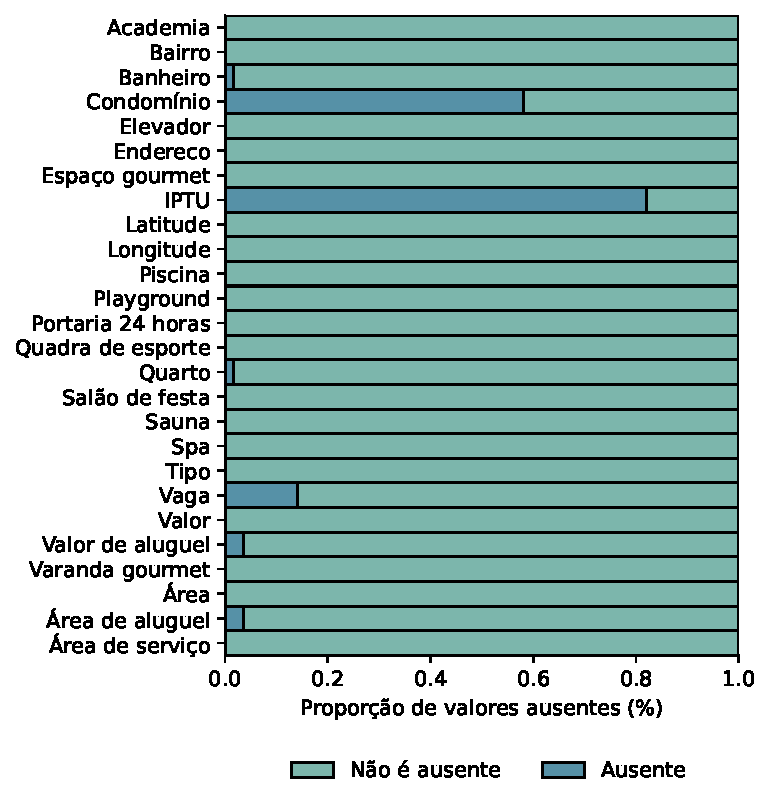
\includegraphics[keepaspectratio]{TCC_files/figure-pdf/fig-miss-output-1.pdf}}

}

\caption{\label{fig-miss}Proporção de valores ausentes por variáveis.}

\end{figure}%

Uma das dificuldades que podem surgir durante a modelagem é o
desbalanceamento das classes, ou seja, a diferença na quantidade de cada
tipo de imóvel. O tipo de imóvel mais predominante no conjunto de dados
de treinamento são os apartamentos, que representam 81,14\% do total. Em
seguida, vêm as casas, com 8,96\%, e os flats, com 5,78\%. As casas de
condomínio são uma das menos representadas, com apenas 2,04\%. Os
terrenos de condomínio e comerciais, somados, representam 2,08\% do
total. Esse desbalanceamento claro entre as classes pode dificultar o
desempenho do modelo, especialmente na predição de categorias menos
frequentes, como as casas de condomínios e terrenos, onde o modelo pode
ter dificuldade em obter bons resultados.

\begin{figure}

\centering{

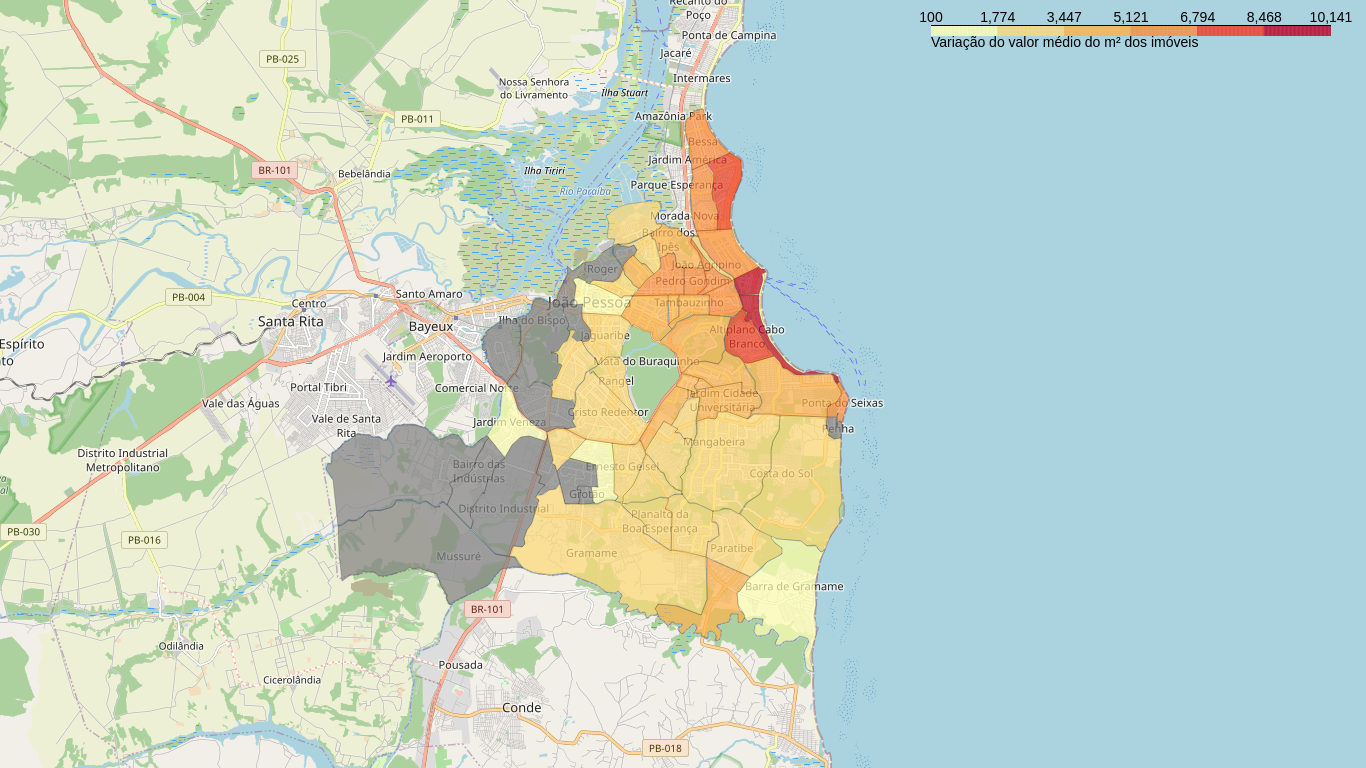
\includegraphics[width=4.6875in,height=2.60417in]{includes/map_valor_m3_final_new.png}

}

\caption{\label{fig-mapa_valor}Variação da média do valor do \(m^2\) dos
imóveis de João Pessoa, área de estudo.}

\end{figure}%

A partir da Figura~\ref{fig-mapa_valor}, tem-se o mapa da região de
estudo, correspondente à cidade de João Pessoa. O mapa apresenta a
variação da média do valor do \(m^2\) dos imóveis, calculada com base
nos bairros da cidade. Vale destacar que alguns bairros não possuíam
dados disponíveis no momento da coleta de informações por raspagem dos
sites de imóveis. Esses bairros estão representados pela cor cinza. Por
outro lado, os bairros com dados disponíveis apresentam variações de
cores que indicam diferentes faixas de valores do \(m^2\). Tonalidades
mais escuras representam bairros com valores médios mais altos para o
\(m^2\), enquanto tonalidades mais claras indicam valores médios
menores.

\vspace{12pt}

O bairro com o maior preço médio do \(m^2\) é Cabo Branco, com um valor
pouco superior a R\$ 10.000,00. Em segundo lugar, está o bairro de
Tambaú, com um valor médio de R\$ 8.951,45 por \(m^2\). Em terceiro,
encontra-se o bairro Jardim Oceania, com um valor médio de R\$ 7.879,60
por \(m^2\), seguido pelo bairro Altiplano Cabo Branco, com um valor
médio de R\$ 7.218,70 por \(m^2\).

\vspace{12pt}

A análise de alguns bairros se torna limitada devido à baixa quantidade
de imóveis disponíveis no momento da raspagem de dados. Por exemplo, o
bairro de Barra de Gramame, que apresenta o menor valor médio de
\(m^2\), tinha apenas um imóvel à venda no momento da coleta de dados.
Da mesma forma, o bairro Jardim Veneza, o segundo com o menor valor
médio por \(m^2\), também possuía poucos registros. Isso indica que os
valores apresentados para esses bairros podem não refletir com precisão
o mercado imobiliário local e podem ser superiores em outras
circunstâncias.

\vspace{12pt}

\begin{figure}

\centering{

\pandocbounded{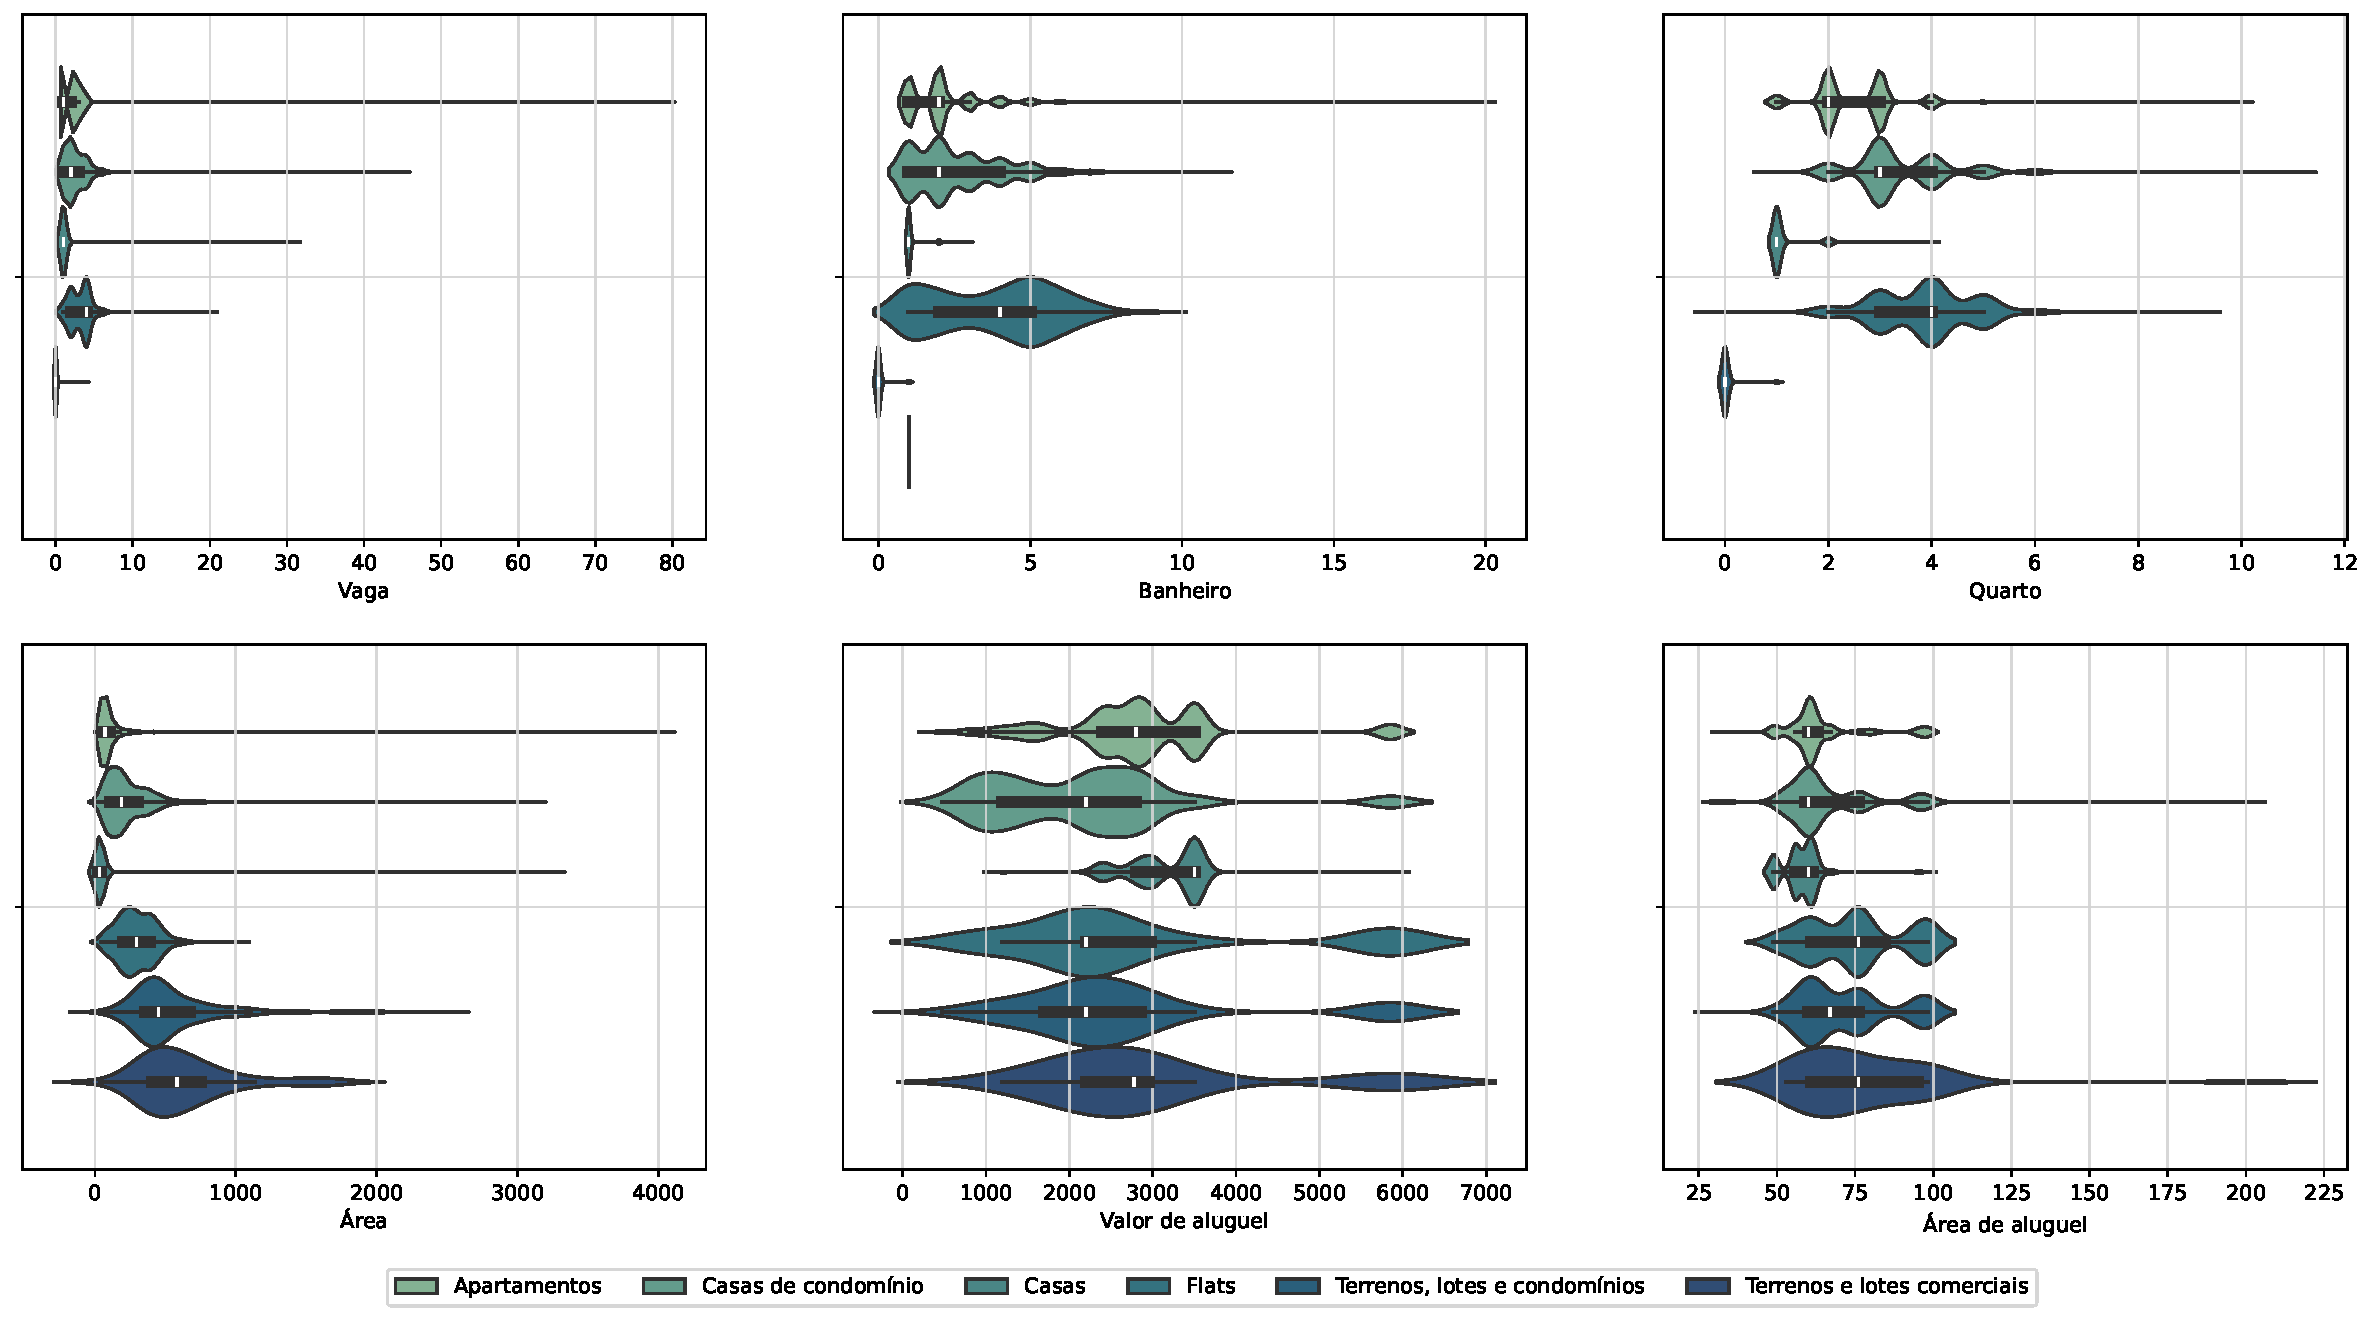
\includegraphics[keepaspectratio]{TCC_files/figure-pdf/fig-violin-output-1.pdf}}

}

\caption{\label{fig-violin}Distribuição das variáveis numéricas.}

\end{figure}%

A distribuição das variáveis foi analisada em termos do tipo do imóvel a
partir de um gráfico de violino. Pela Figura~\ref{fig-violin}, é fácil
perceber que a maioria das distribuições possuem assimetria negativa,
com caudas longas à direita, indicando a presença de valores
extremamente altos e a necessidade da aplicação de alguma transformação
para a estabilização da variância.

\vspace{12pt}

Para reduzir a assimetria da distribuição dos valores dos imóveis, foi
aplicada uma transformação logarítmica \(\log\left(1 + x\right)\). O
gráfico de densidade à esquerda na Figura~\ref{fig-densitarg} mostra a
distribuição do valor dos imóveis. Há uma tendência dos valores ficarem
mais concentrados em uma faixa mais baixa, mas alguns imóveis apresentam
valores excepcionalmente altos, o que acaba gerando uma distribuição
assimétrica positiva. Com a aplicação da transformação logarítmica, a
assimetria é suavizada da distribuição é reduzida.

\begin{figure}

\centering{

\pandocbounded{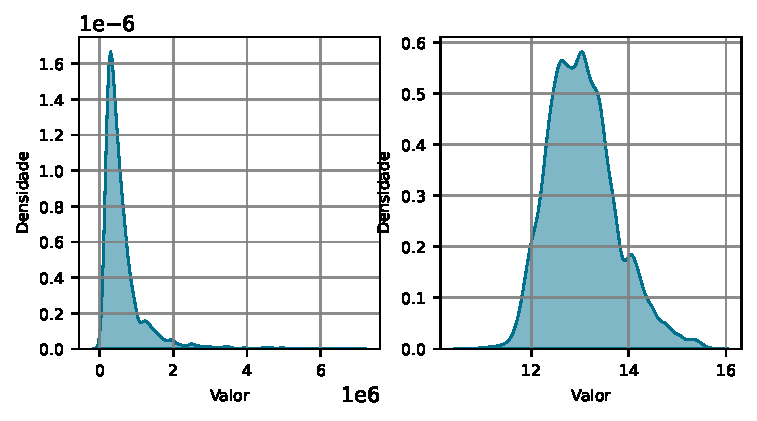
\includegraphics[keepaspectratio]{TCC_files/figure-pdf/fig-densitarg-output-1.pdf}}

}

\caption{\label{fig-densitarg}Comparação entre distribuição dos valores
dos imóveis antes e depois da transformação logarítmica.}

\end{figure}%

\begin{figure}

\centering{

\pandocbounded{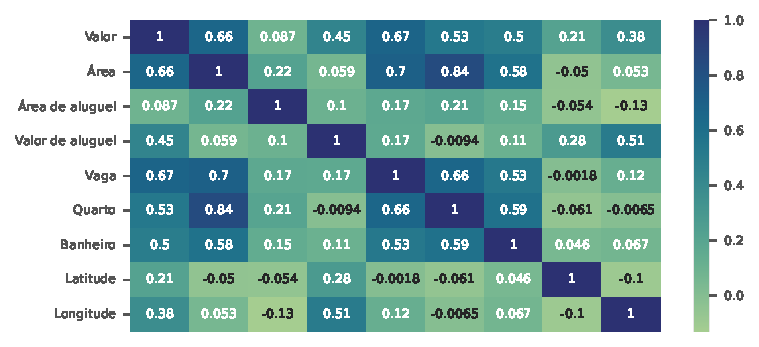
\includegraphics[keepaspectratio]{TCC_files/figure-pdf/fig-corplot-output-1.pdf}}

}

\caption{\label{fig-corplot}Gráfico de correlação de Spearman das
variáveis independentes.}

\end{figure}%

\vspace{12pt}

A Figura~\ref{fig-corplot} apresenta a matriz de correlação entre as
variáveis numéricas do conjunto de dados. As cores mais escuras indicam
uma correlação mais forte entre as variáveis, enquanto as cores mais
claras indicam o contrário. O valor do imóvel apresenta maior correlação
com as variáveis de área do imóvel e número de vagas de estacionamento.
Além disso, o valor do imóvel tem alta correlação com o valor médio do
aluguel, número de quartos e banheiros, além de ser fortemente
influenciado pela localização dos imóveis.

\vspace{12pt}

A partir do gráfico de correlação, foram criadas novas variáveis com
base nas interações entre as mais correlacionadas. Dessa forma, foram
adicionadas trẽs novas variáveis. A primeira é o produto entre o número
de quartos do imóvel e a área média do aluguel no bairro; a segunda
representa a razão entre o número de quartos e a área do imóvel; e a
terceira resulta do produto entre as coordenadas geográficas e o preço
médio do aluguel no bairro. Além disso, foi considerada uma variável que
representa a quantidade total de cômodos do imóvel. Para isso,
somaram-se o número de quartos e banheiros, adicionando-se dois cômodos
a mais para imóveis do tipo apartamento, casa, casa de condomínio e
flat, assumindo a existência de sala e cozinha.

\section{Tunagem dos modelos}\label{tunagem-dos-modelos}

~~~Como os algoritmos utilizados neste trabalho são baseados em árvores
de decisão ou podem utilizar algoritmos baseados em árvore, como Random
Forest, Gradient Boosting e suas variações, os parâmetros escolhidos
para otimização serão bastantes parecidos. Assim, foram ajustados
hiperparâmetros como o número de árvores e a profundidade das árvores,
de forma a capturar a complexidade das relações presentes nos dados.
Além disso, para os algoritmos baseados em Gradient Boosting, o
hiperparâmetro de taxa de aprendizado também foi ajustado.

\vspace{12pt}

Todos os modelos e bibliotecas usados neste trabalho seguem a API do
\href{https://scikit-learn.org/stable/}{\textbf{scikit-learn}}. Nessa
API, o hiperparâmetro que define a quantidade de árvores é denominado
\texttt{n\_estimators}, o de profundidade das árvores é
\texttt{max\_depth}, e o de taxa de aprendizado é
\texttt{learning\_rate}. Com a configuração da função objetivo na
biblioteca \href{https://optuna.org/}{\textbf{Optuna}}, foi possível
encontrar o ponto ótimo desses hiperparâmetros para cada modelo.

\subsection{Tunagem da Random Forest}\label{tunagem-da-random-forest}

~~~Para o modelo Random Forest, a função objetivo foi definida apenas
para otimizar os hiperparâmetros de quantidade de árvores e de
profundidade da árvore. O espaço de procura para a quantidade de árvores
foi definido entre 1 a 1000 árvores. Já o hiperparâmetro de profundidade
da árvore foi definido entre 20 a 1000. Além disso, foi utilizado
aleatoriamente \(m = \sqrt{p}\) das \(p\) variáveis independentes como
candidatas para a divisão.

\begin{figure}

\begin{minipage}{0.50\linewidth}

\centering{

\pandocbounded{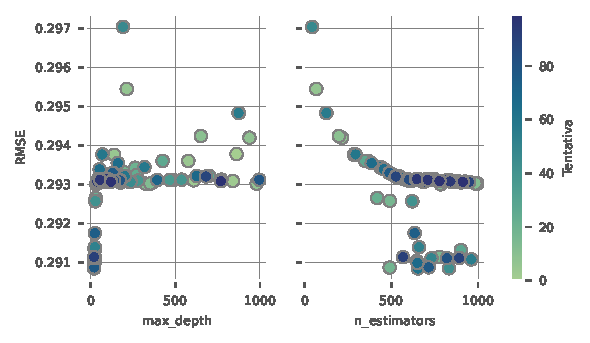
\includegraphics[keepaspectratio]{TCC_files/figure-pdf/fig-rf_slice-output-1.pdf}}

}

\subcaption{\label{fig-rf_slice}}

\end{minipage}%
%
\begin{minipage}{0.50\linewidth}

\centering{

\pandocbounded{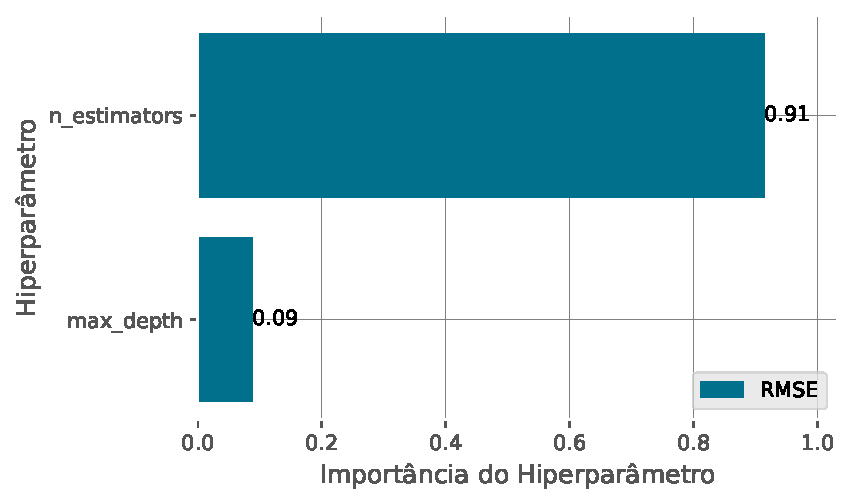
\includegraphics[keepaspectratio]{TCC_files/figure-pdf/fig-rf_import-output-1.pdf}}

}

\subcaption{\label{fig-rf_import}}

\end{minipage}%
\newline
\begin{minipage}{0.50\linewidth}

\centering{

\pandocbounded{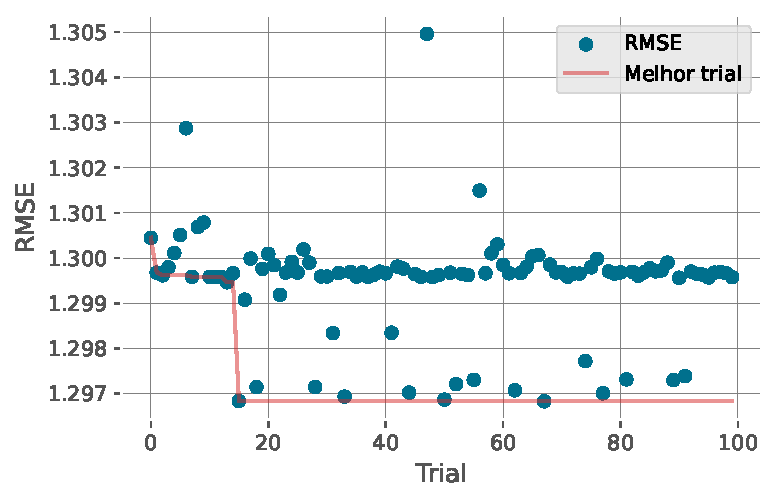
\includegraphics[keepaspectratio]{TCC_files/figure-pdf/fig-rf_history-output-1.pdf}}

}

\subcaption{\label{fig-rf_history}}

\end{minipage}%
%
\begin{minipage}{0.50\linewidth}

\centering{

\pandocbounded{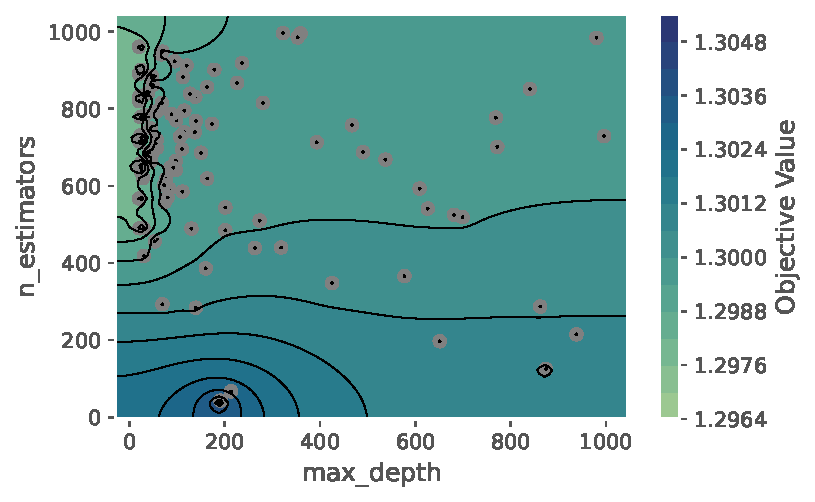
\includegraphics[keepaspectratio]{TCC_files/figure-pdf/fig-rf_contour-output-1.pdf}}

}

\subcaption{\label{fig-rf_contour}}

\end{minipage}%

\caption{\label{fig-rf_param}Resultados da tunagem da Random Forest.}

\end{figure}%

A Figura~\ref{fig-rf_slice} mostra a variação da estatística de erro em
função dos valores de cada hiperparâmetro ao longo dos trials. O gráfico
Figura~\ref{fig-rf_import} exibe a importância de cada hiperparâmetro,
calculada pelo método fANOVA. Na Figura~\ref{fig-rf_history}, observa-se
a variação do erro para cada trial, com a linha vermelha representando o
menor valor obtido em cada etapa. Por fim, a Figura~\ref{fig-rf_contour}
é um gráfico de área que mostra a interação entre os hiperparâmetros
tunados em relação à estatística de erro.

\vspace{12pt}

A partir da Figura~\ref{fig-rf_slice}, é possível ver que o erro tende a
ser menor para valores menores do hiperparâmetro de profundidade das
árvores \texttt{max\_depth}. Em contraste, para o hiperparâmetro de
número de árvores, \texttt{n\_estimators}, o erro apresenta uma
tendência de redução e estabilização à medida que o número de árvores
aumenta. Esse comportamento também é observado na
Figura~\ref{fig-rf_contour}, onde valores menores para
\texttt{max\_depth} e maiores para \texttt{n\_estimators} resultam em um
modelo com menor erro de generalização.

\vspace{12pt}

Além disso, o gráfico de importância dos hiperparâmetros na
Figura~\ref{fig-rf_import} revela que o hiperparâmetro
\texttt{n\_estimators} possui uma maior contribuição na performance do
modelo. A Figura~\ref{fig-rf_history} ilustra o comportamento da métrica
de erro para cada trial, mostrando que o método de otimização alcança um
de seus melhores valores pouco antes do trial 20.

\begin{longtable}[]{@{}cccc@{}}
\caption{Melhores hiperparâmetros para Random
Forest.}\label{tbl-params_rf}\tabularnewline
\toprule\noalign{}
Tentativa & RMSE & n\_estimators & max\_depth \\
\midrule\noalign{}
\endfirsthead
\toprule\noalign{}
Tentativa & RMSE & n\_estimators & max\_depth \\
\midrule\noalign{}
\endhead
\bottomrule\noalign{}
\endlastfoot
62 & 0,29 & 653 & 21 \\
\end{longtable}

\subsection{Tunagem do Gradient
Boosting}\label{tunagem-do-gradient-boosting}

\begin{figure}

\begin{minipage}{0.33\linewidth}

\centering{

\pandocbounded{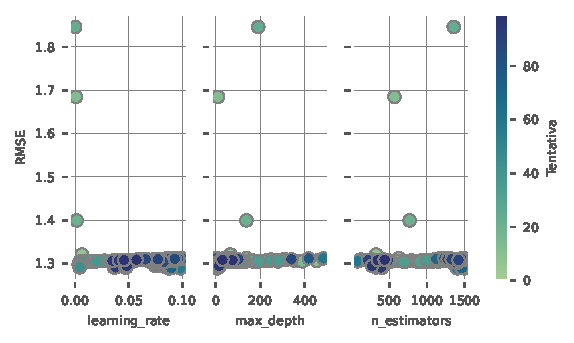
\includegraphics[keepaspectratio]{TCC_files/figure-pdf/fig-gdt_slice-output-1.pdf}}

}

\subcaption{\label{fig-gdt_slice}}

\end{minipage}%
%
\begin{minipage}{0.33\linewidth}

\centering{

\pandocbounded{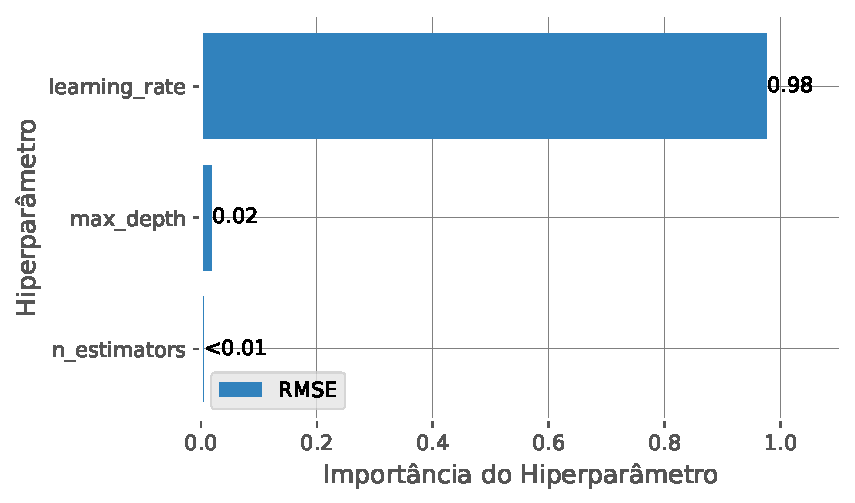
\includegraphics[keepaspectratio]{TCC_files/figure-pdf/fig-gdt_import-output-1.pdf}}

}

\subcaption{\label{fig-gdt_import}}

\end{minipage}%
%
\begin{minipage}{0.33\linewidth}

\centering{

\pandocbounded{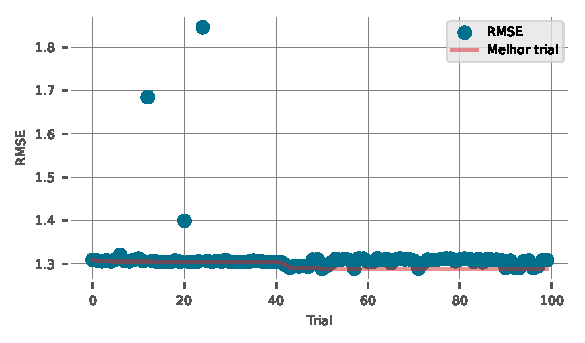
\includegraphics[keepaspectratio]{TCC_files/figure-pdf/fig-gdt_history-output-1.pdf}}

}

\subcaption{\label{fig-gdt_history}}

\end{minipage}%
\newline
\begin{minipage}{\linewidth}

\centering{

\pandocbounded{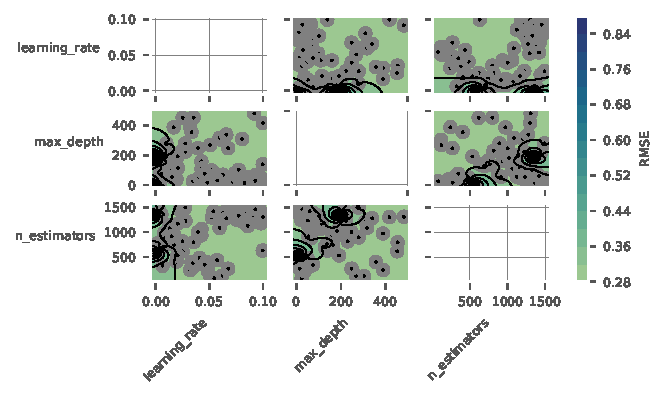
\includegraphics[keepaspectratio]{TCC_files/figure-pdf/fig-gdt_contour-output-1.pdf}}

}

\subcaption{\label{fig-gdt_contour}}

\end{minipage}%

\caption{\label{fig-gdt_param}Resultados da tunagem do Gradient
Boosting.}

\end{figure}%

~~~Para o algoritmo de Gradient Boosting, os hiperparâmetros ajustados
foram a taxa de aprendizado, a quantidade de árvores e a profundidade
das árvores. No \href{https://optuna.org/}{\textbf{Optuna}}, o espaço de
busca definido na função objetivo para a taxa de aprendizado variou de
\(1 \cdot 10^{-5}\) a \(1 \cdot 10^{-1}\); para a profundidade das
árvores, de 3 a 500; e para a quantidade de árvores, de 50 a 1500. Assim
como no Random Forest, foi utilizada \(m = \sqrt{p}\)\hspace{0pt} das
\(p\) variáveis independentes para realizar as divisões nas árvores.

\vspace{12pt}

A análise da importância dos hiperparâmetros, apresentada na
Figura~\ref{fig-gdt_import}, indica que o hiperparâmetro com maior
influência na variação da função objetivo - e, consequentemente, na
performance do modelo - é a taxa de aprendizado. Em seguida, a
profundidade das árvores é a segunda mais relevante, enquanto o número
de árvores tem a menor influência.

\vspace{12pt}

Diferentemente do modelo de Random Forest, o algoritmo de Gradient
Boosting apresentou melhorias significativas, como ilustrado na
Figura~\ref{fig-gdt_history}, em que a estatística de erro foi bastante
estável para cada combinação de hiperparâmetros, além de ter se mantido
abaixo de 0,29 por muitas vezes. A relação entre os hiperparâmetros é
bastante similar à obtida para o Random Forest. Na
Figura~\ref{fig-gdt_contour}, observa-se que o método de otimização TPE
tende a selecionar valores menores para a profundidade das árvores e
maiores para o número de árvores.

\begin{longtable}[]{@{}
  >{\centering\arraybackslash}p{(\linewidth - 8\tabcolsep) * \real{0.1864}}
  >{\centering\arraybackslash}p{(\linewidth - 8\tabcolsep) * \real{0.1356}}
  >{\centering\arraybackslash}p{(\linewidth - 8\tabcolsep) * \real{0.2373}}
  >{\centering\arraybackslash}p{(\linewidth - 8\tabcolsep) * \real{0.1864}}
  >{\centering\arraybackslash}p{(\linewidth - 8\tabcolsep) * \real{0.2542}}@{}}
\caption{Melhores hiperparâmetros para Gradient
Boosting.}\label{tbl-params_gdt}\tabularnewline
\toprule\noalign{}
\begin{minipage}[b]{\linewidth}\centering
Tentativa
\end{minipage} & \begin{minipage}[b]{\linewidth}\centering
RMSE
\end{minipage} & \begin{minipage}[b]{\linewidth}\centering
n\_estimators
\end{minipage} & \begin{minipage}[b]{\linewidth}\centering
max\_depth
\end{minipage} & \begin{minipage}[b]{\linewidth}\centering
learning\_rate
\end{minipage} \\
\midrule\noalign{}
\endfirsthead
\toprule\noalign{}
\begin{minipage}[b]{\linewidth}\centering
Tentativa
\end{minipage} & \begin{minipage}[b]{\linewidth}\centering
RMSE
\end{minipage} & \begin{minipage}[b]{\linewidth}\centering
n\_estimators
\end{minipage} & \begin{minipage}[b]{\linewidth}\centering
max\_depth
\end{minipage} & \begin{minipage}[b]{\linewidth}\centering
learning\_rate
\end{minipage} \\
\midrule\noalign{}
\endhead
\bottomrule\noalign{}
\endlastfoot
57 & 0,28 & 1404 & 7 & \(9,81\times10^{-2}\) \\
\end{longtable}

\subsection{Tunagem do LGBM}\label{tunagem-do-lgbm}

~~~Para a otimização do LGBM, foram considerados os mesmos
hiperparâmetros utilizados no algoritmo Gradient Boosting, com a adição
do ajuste do número máximo de folhas por árvore. O espaço de busca para
o número de árvores foi definido entre 100 e 2000; para a taxa de
aprendizado, utilizou-se o mesmo intervalo adotado no Gradient Boosting;
para o número total de folhas, o intervalo foi de 100 a 600; e, por fim,
para a profundidade das árvores, o intervalo adotado foi de 100 a 500.

\begin{figure}

\begin{minipage}{0.33\linewidth}

\centering{

\pandocbounded{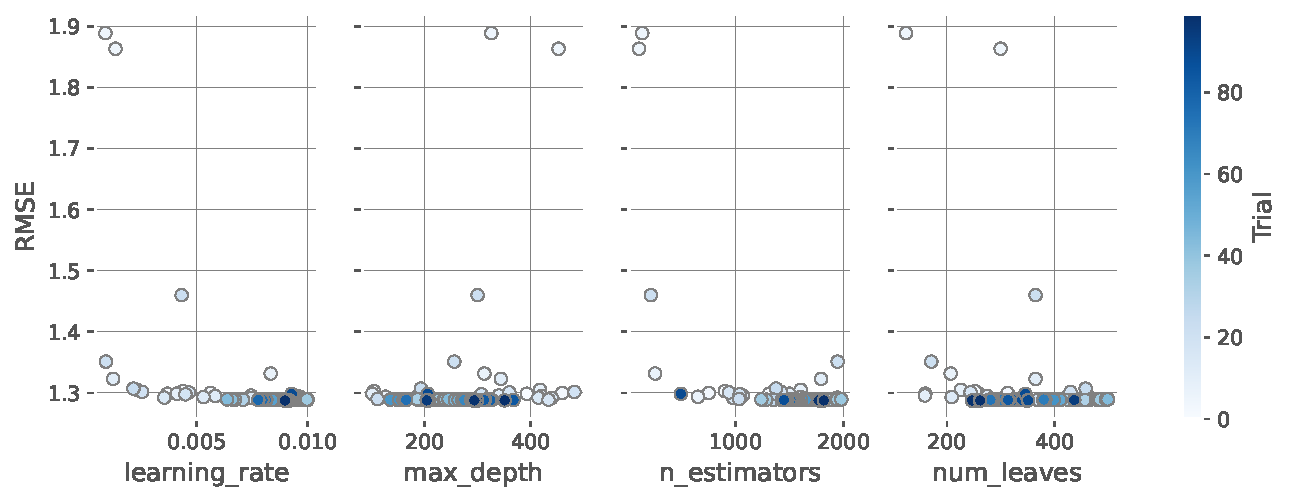
\includegraphics[keepaspectratio]{TCC_files/figure-pdf/fig-lgbm_slice-output-1.pdf}}

}

\subcaption{\label{fig-lgbm_slice}}

\end{minipage}%
%
\begin{minipage}{0.33\linewidth}

\centering{

\pandocbounded{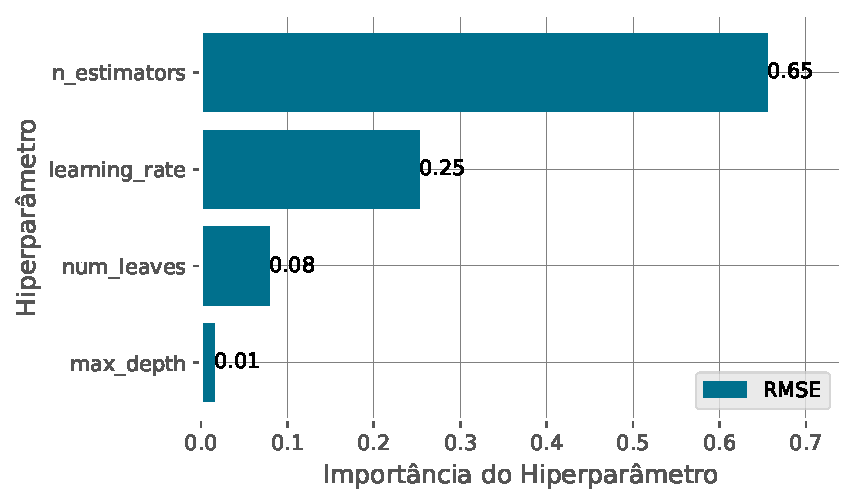
\includegraphics[keepaspectratio]{TCC_files/figure-pdf/fig-lgbm_import-output-1.pdf}}

}

\subcaption{\label{fig-lgbm_import}}

\end{minipage}%
%
\begin{minipage}{0.33\linewidth}

\centering{

\pandocbounded{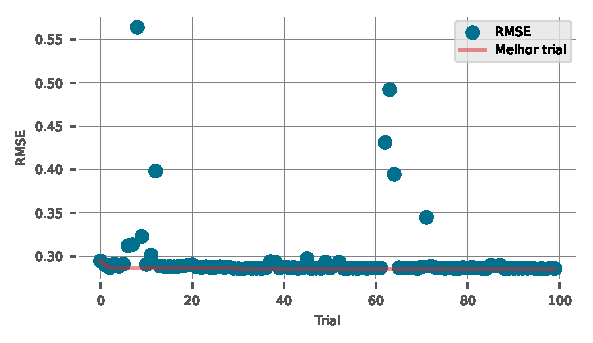
\includegraphics[keepaspectratio]{TCC_files/figure-pdf/fig-lgbm_history-output-1.pdf}}

}

\subcaption{\label{fig-lgbm_history}}

\end{minipage}%
\newline
\begin{minipage}{\linewidth}

\centering{

\pandocbounded{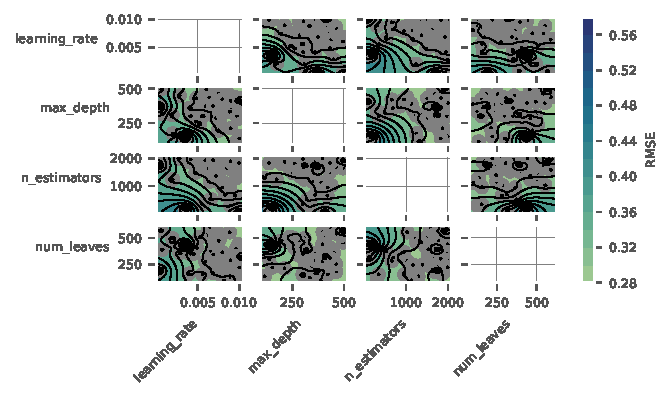
\includegraphics[keepaspectratio]{TCC_files/figure-pdf/fig-lgbm_contour-output-1.pdf}}

}

\subcaption{\label{fig-lgbm_contour}}

\end{minipage}%

\caption{\label{fig-lgbm_param}Resultados da tunagem do LGBM.}

\end{figure}%

\vspace{12pt}

As trials de otimização do modelo LGBM (Figura~\ref{fig-lgbm_history})
apresentaram um comportamento semelhante ao do Gradient Boosting, porém
com menor estabilidade em cada tentativa. Ao analisar a contribuição de
cada hiperparâmetro para o desempenho do modelo na
Figura~\ref{fig-lgbm_import}, observa-se que a taxa de aprendizado e a
quantidade de árvores são os hiperparâmetros de maior influência,
seguidos pela quantidade total de folhas e, por último, a profundidade
máxima da árvore.

\vspace{12pt}

Analisando a relação entre o hiperparâmetro de profundidade da árvore e
o número de folhas em função da estatística de erro na
Figura~\ref{fig-lgbm_contour}, observa-se que uma menor quantidade de
folhas e uma maior profundidade das árvores resultam em um modelo com
menor erro. Para uma maior quantidade de árvores e uma taxa de
aprendizado tendendo a 0,01, a estatística de erro apresenta diminuição.

\begin{longtable}[]{@{}
  >{\centering\arraybackslash}p{(\linewidth - 10\tabcolsep) * \real{0.1549}}
  >{\centering\arraybackslash}p{(\linewidth - 10\tabcolsep) * \real{0.1127}}
  >{\centering\arraybackslash}p{(\linewidth - 10\tabcolsep) * \real{0.1972}}
  >{\centering\arraybackslash}p{(\linewidth - 10\tabcolsep) * \real{0.1690}}
  >{\centering\arraybackslash}p{(\linewidth - 10\tabcolsep) * \real{0.1549}}
  >{\centering\arraybackslash}p{(\linewidth - 10\tabcolsep) * \real{0.2113}}@{}}
\caption{Melhores hiperparâmetros para Light Gradient
Boosting.}\label{tbl-params_lgbm}\tabularnewline
\toprule\noalign{}
\begin{minipage}[b]{\linewidth}\centering
Tentativa
\end{minipage} & \begin{minipage}[b]{\linewidth}\centering
RMSE
\end{minipage} & \begin{minipage}[b]{\linewidth}\centering
n\_estimators
\end{minipage} & \begin{minipage}[b]{\linewidth}\centering
num\_leaves
\end{minipage} & \begin{minipage}[b]{\linewidth}\centering
max\_depth
\end{minipage} & \begin{minipage}[b]{\linewidth}\centering
learning\_rate
\end{minipage} \\
\midrule\noalign{}
\endfirsthead
\toprule\noalign{}
\begin{minipage}[b]{\linewidth}\centering
Tentativa
\end{minipage} & \begin{minipage}[b]{\linewidth}\centering
RMSE
\end{minipage} & \begin{minipage}[b]{\linewidth}\centering
n\_estimators
\end{minipage} & \begin{minipage}[b]{\linewidth}\centering
num\_leaves
\end{minipage} & \begin{minipage}[b]{\linewidth}\centering
max\_depth
\end{minipage} & \begin{minipage}[b]{\linewidth}\centering
learning\_rate
\end{minipage} \\
\midrule\noalign{}
\endhead
\bottomrule\noalign{}
\endlastfoot
31 & 0,28 & 1988 & 202 & 379 & \(9,85\times10^{-3}\) \\
\end{longtable}

\subsection{Tunagem do XGBoost}\label{tunagem-do-xgboost}

~~~Para o algoritmo Extreme Gradient Boosting, os hiperparâmetros
selecionados para a tunagem foram a taxa de aprendizagem, profundidade
da árvore e quantidade máxima de árvores. Na configuração da função
objetivo para a tunagem dos hiperparâmetros pelo optuna, a taxa de
aprendizagem variou entre \(1 \cdot 10^{-7}\) e \(0.5\), a profundidade
da árvore variou entre 3 e 50 e a quantidade de árvores variou entre 50
e 1000.

\vspace{12pt}

A partir da Figura~\ref{fig-xgb_import}, o hiperparâmetro que
representou a maior variação na função objetivo, e portanto a maior
importância para a performance do modelo, foi a taxa de aprendizagem. A
profundidade da árvore permanece como o segundo hiperparâmetro mais
relevante, seguida pela quantidade de árvores, que ocupa a última
posição em termos de importância. Observando a
Figura~\ref{fig-xgb_history}, é possível ver que o algoritmo de XGBoost
foi aquele que apresentou a menor variação entre as trials, com uma
única trial com erro acima de 1,0.

\vspace{12pt}

O algoritmo de otimização TPE apresentou uma maior frequência de procura
do hiperparâmetro de taxa de aprendizagem para valores menores, como
pode ser visto na Figura~\ref{fig-xgb_slice}. O mesmo acontece para o
hiperparâmetro de profundidade de árvores, há uma repetição maior para
valores menores, indicando que a estatística de erro tendeu a ter
valores menores para essa região. Para a quantidade de árvores, esse
padrão foi diferente, uma quantidade maior de árvores faz com que o
modelo tenha um melhor ajuste. Essas relações também podem ser
observadas a partir da Figura~\ref{fig-xgb_contour}, menores taxas de
aprendizado, combinadas com uma menor profundidade de árvore e maior
quantidade de árvores apresentam menor valor na função objetivo.

\begin{figure}

\begin{minipage}{0.33\linewidth}

\centering{

\pandocbounded{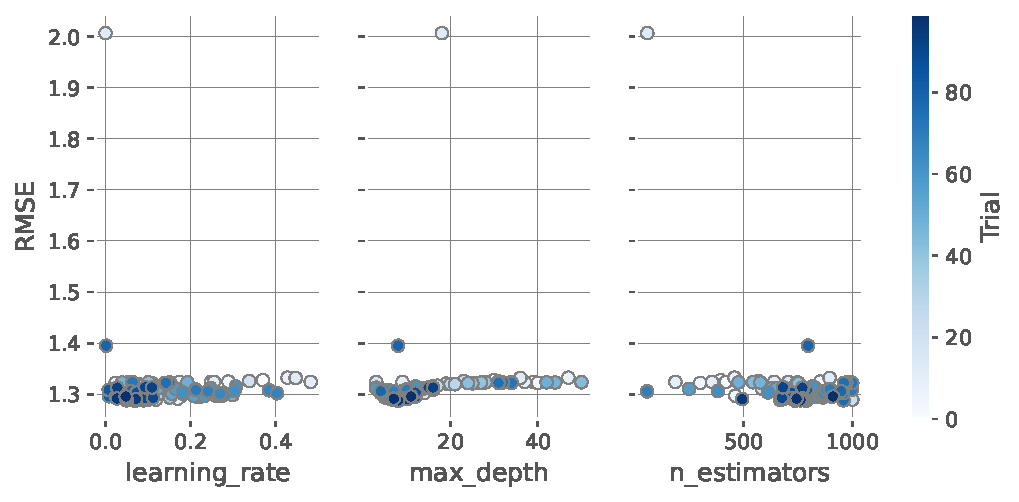
\includegraphics[keepaspectratio]{TCC_files/figure-pdf/fig-xgb_slice-output-1.pdf}}

}

\subcaption{\label{fig-xgb_slice}}

\end{minipage}%
%
\begin{minipage}{0.33\linewidth}

\centering{

\pandocbounded{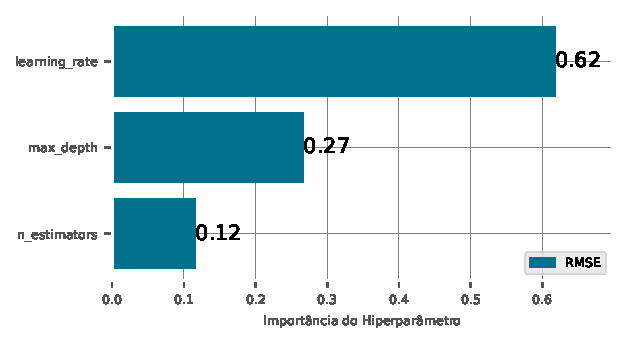
\includegraphics[keepaspectratio]{TCC_files/figure-pdf/fig-xgb_import-output-1.pdf}}

}

\subcaption{\label{fig-xgb_import}}

\end{minipage}%
%
\begin{minipage}{0.33\linewidth}

\centering{

\pandocbounded{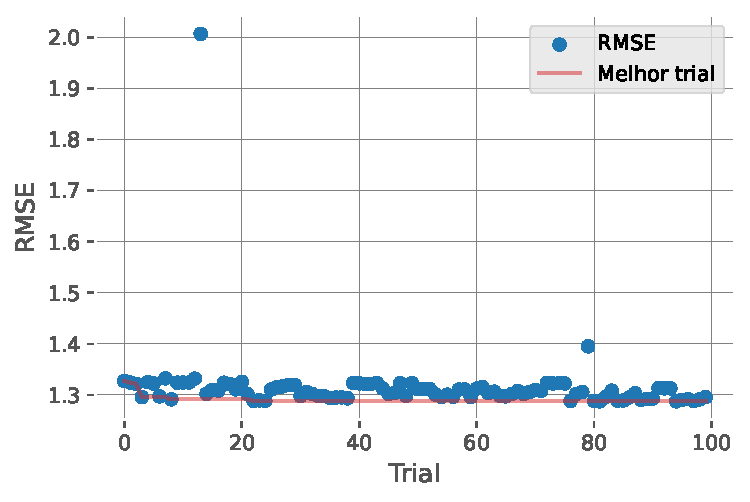
\includegraphics[keepaspectratio]{TCC_files/figure-pdf/fig-xgb_history-output-1.pdf}}

}

\subcaption{\label{fig-xgb_history}}

\end{minipage}%
\newline
\begin{minipage}{\linewidth}

\centering{

\pandocbounded{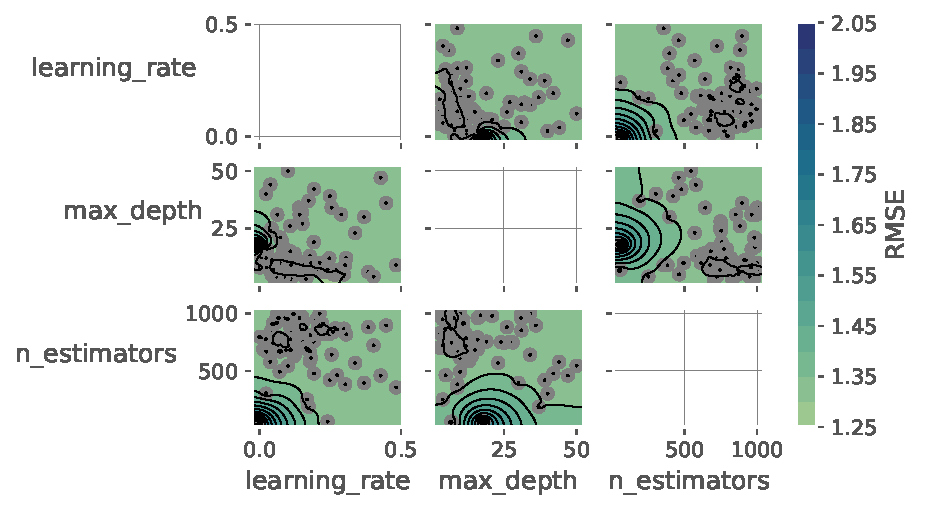
\includegraphics[keepaspectratio]{TCC_files/figure-pdf/fig-xgb_contour-output-1.pdf}}

}

\subcaption{\label{fig-xgb_contour}}

\end{minipage}%

\caption{\label{fig-xgb_param}Resultados da tunagem do XGBoost.}

\end{figure}%

\begin{longtable}[]{@{}
  >{\centering\arraybackslash}p{(\linewidth - 8\tabcolsep) * \real{0.1864}}
  >{\centering\arraybackslash}p{(\linewidth - 8\tabcolsep) * \real{0.1356}}
  >{\centering\arraybackslash}p{(\linewidth - 8\tabcolsep) * \real{0.2373}}
  >{\centering\arraybackslash}p{(\linewidth - 8\tabcolsep) * \real{0.1864}}
  >{\centering\arraybackslash}p{(\linewidth - 8\tabcolsep) * \real{0.2542}}@{}}
\caption{Melhores hiperparâmetros para Extreme Gradient
Boosting.}\label{tbl-params_xgb}\tabularnewline
\toprule\noalign{}
\begin{minipage}[b]{\linewidth}\centering
Tentativa
\end{minipage} & \begin{minipage}[b]{\linewidth}\centering
RMSE
\end{minipage} & \begin{minipage}[b]{\linewidth}\centering
n\_estimators
\end{minipage} & \begin{minipage}[b]{\linewidth}\centering
max\_depth
\end{minipage} & \begin{minipage}[b]{\linewidth}\centering
learning\_rate
\end{minipage} \\
\midrule\noalign{}
\endfirsthead
\toprule\noalign{}
\begin{minipage}[b]{\linewidth}\centering
Tentativa
\end{minipage} & \begin{minipage}[b]{\linewidth}\centering
RMSE
\end{minipage} & \begin{minipage}[b]{\linewidth}\centering
n\_estimators
\end{minipage} & \begin{minipage}[b]{\linewidth}\centering
max\_depth
\end{minipage} & \begin{minipage}[b]{\linewidth}\centering
learning\_rate
\end{minipage} \\
\midrule\noalign{}
\endhead
\bottomrule\noalign{}
\endlastfoot
81 & 0,28 & 788 & 8 & \(7,12\times10^{-2}\) \\
\end{longtable}

A Tabela~\ref{tbl-params_xgb} apresenta a tentativa em que a combinação
de hiperparâmetros resultou no menor erro para o algoritmo de Extreme
Gradient Boosting. Nesse caso, a melhor tentativa foi a de número 81,
com uma configuração de 788 árvores, profundidade máxima igual a 8 e
taxa de aprendizado de \(7,12\times10^{-2}\).

\vspace{12pt}

Para o LGBM, a melhor combinação foi encontrada na tentativa 31, com
1.988 árvores, quantidade máxima de 202 folhas, profundidade máxima de
379 e taxa de aprendizado de \(9,85\times10^{-3}\), como apresentado na
Tabela~\ref{tbl-params_lgbm}.

\vspace{12pt}

Por fim, para os algoritmos Gradient Boosting e Random Forest, as
melhores tentativas foram as de números 57 e 62, respectivamente. No
caso do Gradient Boosting, a configuração ideal foi composta por 1.404
árvores, profundidade máxima de 7 e taxa de aprendizado de
\(9,81\times10^{-2}\). Já para o Random Forest, a melhor combinação
consistiu em 653 árvores e profundidade máxima de 21. Os resultados
estão na Tabela~\ref{tbl-params_gdt} e Tabela~\ref{tbl-params_rf},
respectivamente.

\section{Resultados dos modelos}\label{resultados-dos-modelos}

~~~Nesta seção, serão apresentados os resultados do ajuste de cada
algoritmo utilizado: Random Forest, Gradient Boosting, LightGBM e
Extreme Gradient Boosting. A análise do ajuste foi realizada com base no
gráfico que compara os valores estimados aos valores observados dos
imóveis. Além disso, foram utilizadas métricas de erro, como MAPE,
\(R^2\) e RMSE, para avaliar o desempenho dos modelos. Os resultados dos
modelos, avaliados no conjunto de teste, podem ser observados na
Tabela~\ref{tbl-metrics_models}.

\vspace{12pt}

O ajuste do algoritmo Random Forest é apresentado na
Figura~\ref{fig-preds_rf}, que exibe a comparação entre os valores
previstos e observados. A raiz do erro quadrático médio (RMSE) foi de
234471,51, enquanto o coeficiente de determinação \(R^2\) alcançou
\(84,54\%\). Em relação ao MAPE, o valor foi de 18,32\%, assim, em
média, as predições realizadas pelo modelo Random Forest, estiveram em
média 18,32\% distantes dos valores reais.

\begin{longtable}[]{@{}
  >{\centering\arraybackslash}p{(\linewidth - 6\tabcolsep) * \real{0.4821}}
  >{\centering\arraybackslash}p{(\linewidth - 6\tabcolsep) * \real{0.1607}}
  >{\centering\arraybackslash}p{(\linewidth - 6\tabcolsep) * \real{0.1964}}
  >{\centering\arraybackslash}p{(\linewidth - 6\tabcolsep) * \real{0.1607}}@{}}
\caption{Métricas obtidas de cada algoritmo no conjunto de
teste.}\label{tbl-metrics_models}\tabularnewline
\toprule\noalign{}
\begin{minipage}[b]{\linewidth}\centering
Algoritmo
\end{minipage} & \begin{minipage}[b]{\linewidth}\centering
RMSE
\end{minipage} & \begin{minipage}[b]{\linewidth}\centering
\(R^2 \ \left(\%\right)\)
\end{minipage} & \begin{minipage}[b]{\linewidth}\centering
MAPE \(\left(\%\right)\)
\end{minipage} \\
\midrule\noalign{}
\endfirsthead
\toprule\noalign{}
\begin{minipage}[b]{\linewidth}\centering
Algoritmo
\end{minipage} & \begin{minipage}[b]{\linewidth}\centering
RMSE
\end{minipage} & \begin{minipage}[b]{\linewidth}\centering
\(R^2 \ \left(\%\right)\)
\end{minipage} & \begin{minipage}[b]{\linewidth}\centering
MAPE \(\left(\%\right)\)
\end{minipage} \\
\midrule\noalign{}
\endhead
\bottomrule\noalign{}
\endlastfoot
Gradient Boosting & 227677,44 & 85,42 & 18,21 \\
Extreme Gradient Boosting & 228300,83 & 85,34 & 18,13 \\
Stacking & 228377,11 & 85,33 & 18,32 \\
Light Gradient Boosting & 228784,37 & 85,28 & 18,34 \\
Random Forest & 234471,51 & 84,54 & 18,32 \\
\end{longtable}

Em relação ao algoritmo de Gradient Boosting, o modelo consegue explicar
\(85,42\%\) da variação da variável dependente, um valor superior ao
obtido com o ajuste do algoritmo de Random Forest, embora a diferença
não seja significante. Para o MAPE, o valor encontrado foi de
\(18,21\%\), indicando que os valores estimados dos imóveis estão, em
média, \(18,21\%\) distantes dos seus valores observados. O seu RMSE foi
de \(227677,44\). A relação entre os valores estimados e os observados
pode ser visualizada na Figura~\ref{fig-preds_gdt}.

\begin{figure}

\begin{minipage}{0.50\linewidth}

\centering{

\pandocbounded{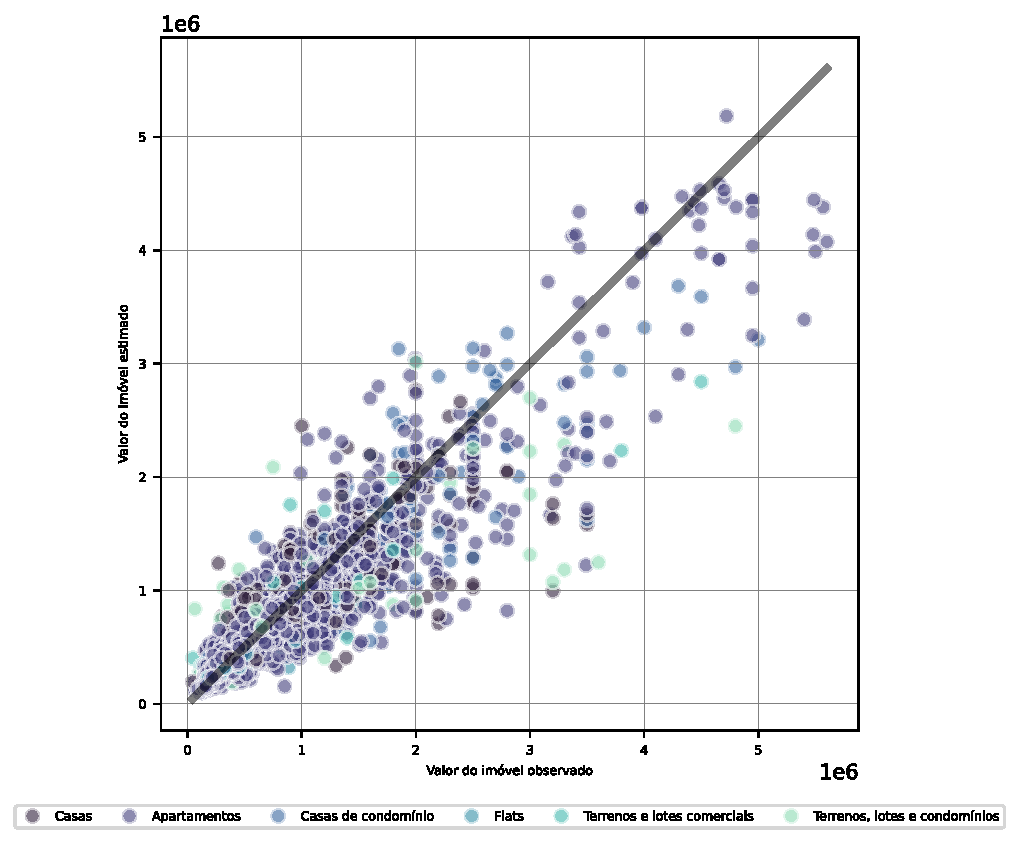
\includegraphics[keepaspectratio]{TCC_files/mediabag/includes/rf_plot_predict_no_transform.pdf}}

}

\subcaption{\label{fig-preds_rf}}

\end{minipage}%
%
\begin{minipage}{0.50\linewidth}

\centering{

\pandocbounded{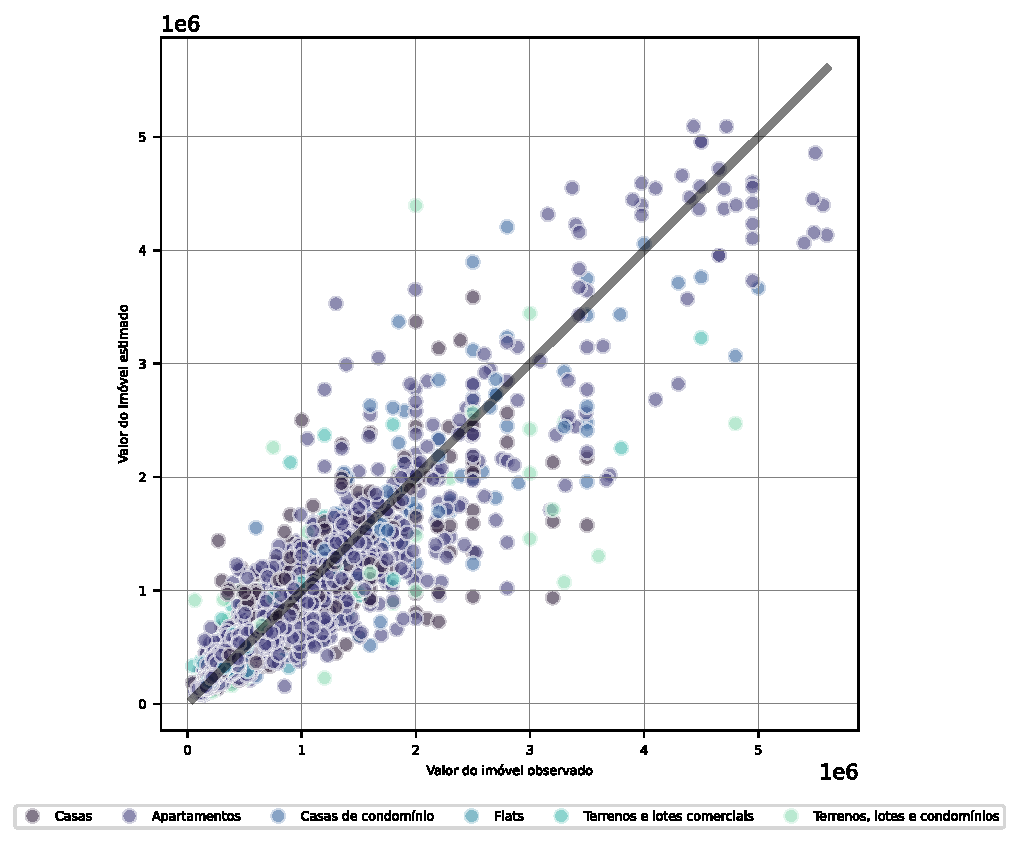
\includegraphics[keepaspectratio]{TCC_files/mediabag/includes/gdt_plot_predict_no_transform.pdf}}

}

\subcaption{\label{fig-preds_gdt}}

\end{minipage}%

\caption{\label{fig-preds1}Valores previstos em função dos observados do
algoritmo Random Forest e Gradient Boosting, respectivamente.}

\end{figure}%

\begin{figure}

\begin{minipage}{0.50\linewidth}

\centering{

\pandocbounded{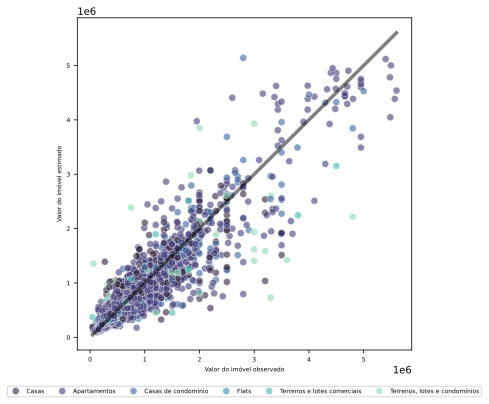
\includegraphics[keepaspectratio]{TCC_files/mediabag/includes/lgbm_plot_predict_no_transform.pdf}}

}

\subcaption{\label{fig-preds_lgbm}}

\end{minipage}%
%
\begin{minipage}{0.50\linewidth}

\centering{

\pandocbounded{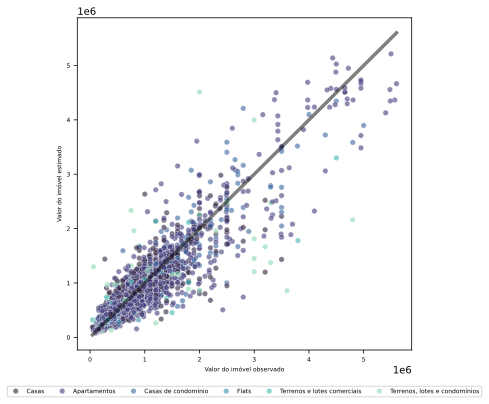
\includegraphics[keepaspectratio]{TCC_files/mediabag/includes/xgb_plot_predict_no_transform.pdf}}

}

\subcaption{\label{fig-preds_xgb}}

\end{minipage}%

\caption{\label{fig-preds2}Valores previstos em função dos observados do
algoritmo Light Gradient Boosting e Extreme Gradient Boosting,
respectivamente.}

\end{figure}%

O Light Gradient Boosting conseguiu melhorias em relação aos resultados
obtidos da Random Forest, mas não em relação ao Gradient Boosting. Em
relação ao seu \(R^2\), o modelo consegue explicar \(85,28\%\) da
variância da variável dependente. O seu RMSE ficou em \(228784,37\) e o
MAPE em \(18,34\%\). Dessa forma, as predições geradas pelo Light
Gradient Boosting estão, em média, \(18,34\%\) distantes de seus valores
reais. O gráfico de seus valores estimados em função dos observados pode
ser observado na Figura~\ref{fig-preds_lgbm}.

\vspace{12pt}

Assim como o LGBM, o Extreme Gradient Boosting também obteve resultados
melhores que o algoritmo de Random Forest. Além disso, foi o modelo que
obteve o melhor MAPE. O RMSE obtido pelo XGBoost foi de \(228300,83\) e
o seu \(R^2\) foi de \(85,34\%\), indicando que o modelo consegue
explicar \(85,34\%\) da variação da variável dependente. As predições
geradas pelo Extreme Gradient Boosting estão, em média, \(18,13\%\)
distantes de seus valores reais.

\vspace{12pt}

Utilizando os modelos finais com hiperparâmetros otimizados, eles foram
combinados como estimadores base para o ajuste do modelo de Stacking. As
estimativas geradas por esse método apresentaram um dos melhores
desempenhos em termos das métricas de erro RMSE e \(R^2\). O RMSE obtido
foi de \(228377,11\), e o modelo foi capaz de explicar \(85,33\%\) da
variância da variável dependente. No geral, os algoritmos apresentaram
métricas bastante semelhantes.

\begin{figure}

\centering{

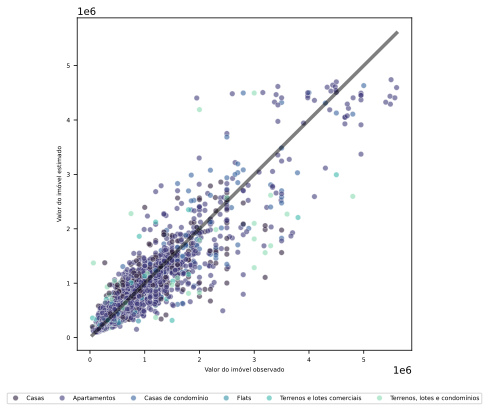
\includegraphics[width=\linewidth,height=3.125in,keepaspectratio]{TCC_files/mediabag/includes/stacking_plot_predict_no_transform.pdf}

}

\caption{\label{fig-preds_stacking}Valores previstos em função dos
observados do algoritmo Stacking.}

\end{figure}%

Nos gráficos das predições geradas pelo modelo, observa-se também que os
maiores desvios ocorrem nos imóveis do tipo terreno, o que pode indicar
a necessidade de um tratamento específico para esse tipo de imóvel. Além
disso, há uma maior variabilidade nos erros de predição para imóveis de
alto valor, sugerindo que o modelo apresenta menor precisão nessas
faixas de preço.

\vspace{12pt}

Embora o Extreme Gradient Boosting tenha apresentado o menor MAPE entre
os algoritmos avaliados, a métrica adotada para a seleção do modelo com
melhor desempenho foi o RMSE, conforme justificado ao final da
Seção~\ref{sec-val_cruz}, no qual o Gradient Boosting se destacou.
Assim, as análises a seguir serão baseadas nesse algoritmo, que também
será utilizado para as previsões na aplicação final.

\section{Impacto e importância das variáveis na
predição}\label{impacto-e-importuxe2ncia-das-variuxe1veis-na-prediuxe7uxe3o}

~~~O impacto e a importância das variáveis na predição de modelos são
fundamentais para entender quais fatores exercem maior influência sobre
as previsões, neste caso, para as predições de valores de imóveis. Esta
seção será dedicada à discussão do impacto das predições individuais e
da importância das variáveis utilizadas na construção do modelo. A
análise será feita com o modelo que apresentou os melhores resultados, o
algoritmo de Gradient Boosting.

\begin{figure}

\centering{

\pandocbounded{\includegraphics[keepaspectratio]{TCC_files/mediabag/includes/pdp_ice2.pdf}}

}

\caption{\label{fig-ice_pdp}Gráfico de ICE e PDP.}

\end{figure}%

Para analisar a influência das variáveis na predição dos valores de
imóveis, foi utilizado o gráfico de ICE em conjunto com a linha de PDP.
Esses gráficos estão representados na Figura~\ref{fig-ice_pdp}.

\vspace{12pt}

As previsões indicam um aumento claro nos valores estimados à medida que
a área do imóvel cresce, com o PDP apresentando uma tendência crescente,
em concordância com as curvas ICE. Para a quantidade de banheiros,
observa-se uma relação majoritariamente estável, com apenas pequenas
variações, comportamento semelhante ao verificado para o número de
quartos, o que pode sugerir uma influência limitada dessas variáveis no
modelo. No entanto, embora essas relações sejam bastante estáveis,
observa-se um aumento nas predições do modelo à medida que cresce a
quantidade de banheiros e quartos.

\vspace{12pt}

No caso do valor médio do aluguel, o PDP revela uma tendência crescente,
reforçada pelas curvas ICE, indicando que aluguéis mais altos estão
fortemente associados a imóveis de maior valor. Por outro lado, a área
média de aluguel apresenta um padrão mais uniforme, sinalizando uma
contribuição menos expressiva na explicação dos preços dos imóveis.

\vspace{12pt}

As curvas ICE para as coordenadas geográficas exibem um comportamento
mais complexo, mas é possível identificar um aumento nos valores
previstos à medida que as coordenadas aumentam. Esse padrão sugere que
imóveis localizados mais próximos da região litorânea de João Pessoa
tendem a ter preços mais elevados. Por fim, a quantidade de vagas de
garagem apresenta uma relação claramente ascendente nas predições.

\begin{figure}

\begin{minipage}{0.50\linewidth}

\centering{

\pandocbounded{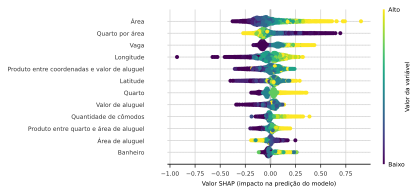
\includegraphics[keepaspectratio]{TCC_files/mediabag/includes/shap_summary_plot2.pdf}}

}

\subcaption{\label{fig-shap_summary}Gráfico de resumo dos valores SHAP.}

\end{minipage}%
%
\begin{minipage}{0.50\linewidth}

\centering{

\pandocbounded{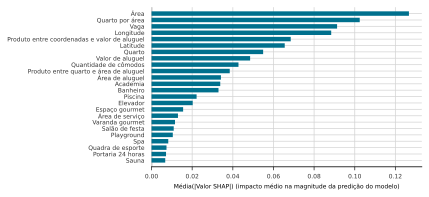
\includegraphics[keepaspectratio]{TCC_files/mediabag/includes/shap_importance2.pdf}}

}

\subcaption{\label{fig-shap_importance}Importância das variáveis.}

\end{minipage}%

\caption{\label{fig-teste}Impacto e importância das variáveis na
predição a partir do método SHAP.}

\end{figure}%

\vspace{12pt}

A análise da importância das variáveis foi realizada por meio do método
SHAP. Diferentemente das medidas tradicionais de importância geradas por
algoritmos baseados em árvores, que se baseiam na redução da impureza, o
SHAP calcula a contribuição de cada variável com base na magnitude dos
valores de Shapley atribuídos individualmente às predições.

\vspace{12pt}

Como pode ser observado na Figura~\ref{fig-shap_importance}, a variável
com maior impacto na predição do modelo é a área do imóvel, responsável
por alterar, em média, mais de 12 pontos percentuais na predição
absoluta. Outras variáveis que se destacam entre as mais relevantes para
a estimativa do valor dos imóveis incluem a quantidade de vagas de
garagem, a razão entre o número de quartos e a área, a localização
geográfica e o produto entre as coordenadas geográficas e o valor do
aluguel. Por último, as quatro variáveis com menor impacto na predição
do modelo são sauna, portaria 24 horas, quadra de esporte e spa.

\vspace{12pt}

Com a Figura~\ref{fig-shap_summary}, observa-se um resumo da análise dos
valores Shapley. A variável área se destaca como a de maior impacto no
modelo, especialmente para valores elevados, que aumentam
significativamente as predições. As coordenadas geográficas indicam que
valores mais altos tendem a elevar a predição do valor dos imóveis,
refletindo a valorização de imóveis localizados mais próximos às regiões
litorâneas de João Pessoa, como observado na Figura~\ref{fig-ice_pdp}.
Por outro lado, a variável de área média de aluguel do bairro apresenta
um padrão menos linear, com valores altos indicando uma redução na
predição do modelo.

\begin{figure}

\begin{minipage}{0.33\linewidth}
\pandocbounded{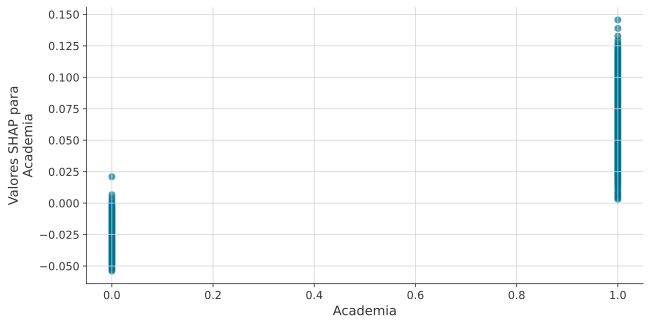
\includegraphics[keepaspectratio]{TCC_files/mediabag/includes/dependence_plot_cat/dep_plot_academia2.pdf}}\end{minipage}%
%
\begin{minipage}{0.33\linewidth}
\pandocbounded{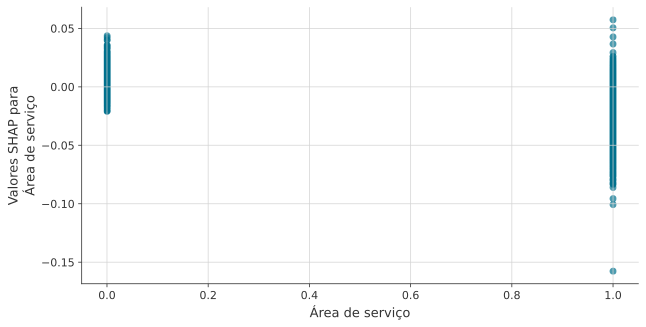
\includegraphics[keepaspectratio]{TCC_files/mediabag/includes/dependence_plot_cat/dep_plot_area_servico2.pdf}}\end{minipage}%
%
\begin{minipage}{0.33\linewidth}
\pandocbounded{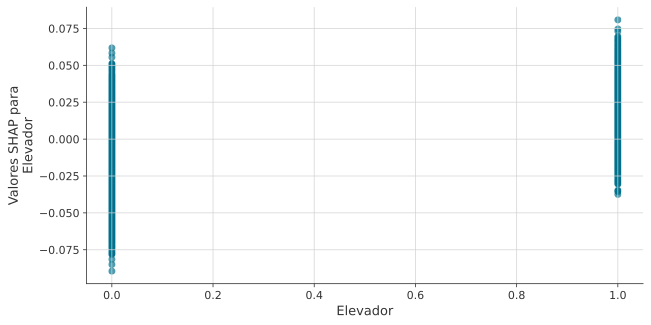
\includegraphics[keepaspectratio]{TCC_files/mediabag/includes/dependence_plot_cat/dep_plot_elevador2.pdf}}\end{minipage}%
\newline
\begin{minipage}{0.33\linewidth}
\pandocbounded{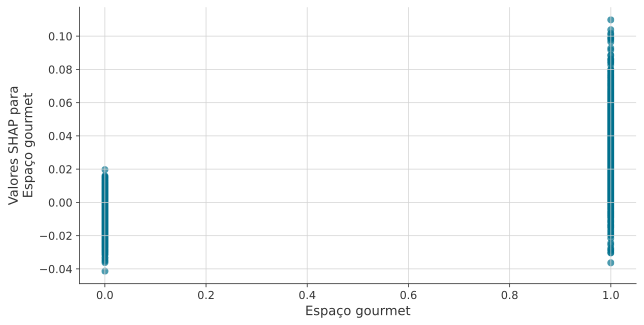
\includegraphics[keepaspectratio]{TCC_files/mediabag/includes/dependence_plot_cat/dep_plot_espaco_gourmet2.pdf}}\end{minipage}%
%
\begin{minipage}{0.33\linewidth}
\pandocbounded{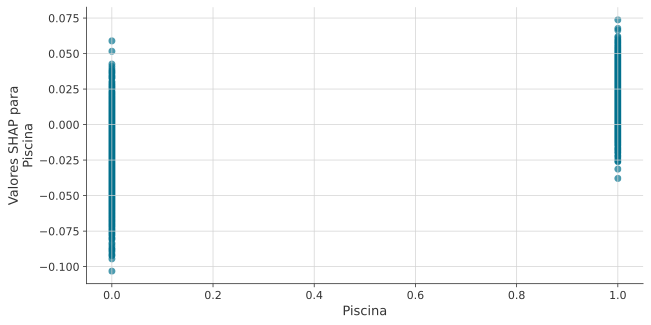
\includegraphics[keepaspectratio]{TCC_files/mediabag/includes/dependence_plot_cat/dep_plot_piscina2.pdf}}\end{minipage}%
%
\begin{minipage}{0.33\linewidth}
\pandocbounded{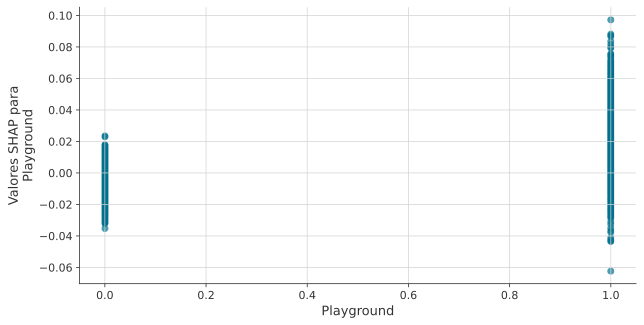
\includegraphics[keepaspectratio]{TCC_files/mediabag/includes/dependence_plot_cat/dep_plot_playground2.pdf}}\end{minipage}%
\newline
\begin{minipage}{0.33\linewidth}
\pandocbounded{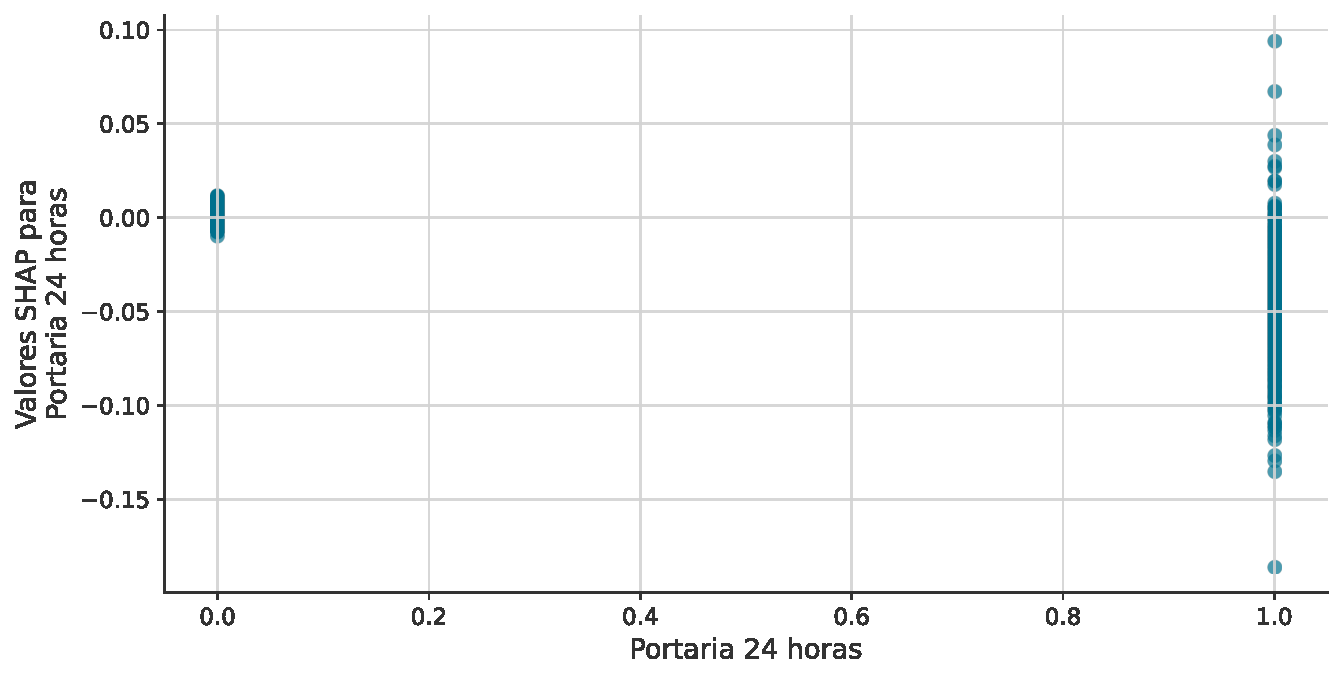
\includegraphics[keepaspectratio]{TCC_files/mediabag/includes/dependence_plot_cat/dep_plot_portaria_24_horas2.pdf}}\end{minipage}%
%
\begin{minipage}{0.33\linewidth}
\pandocbounded{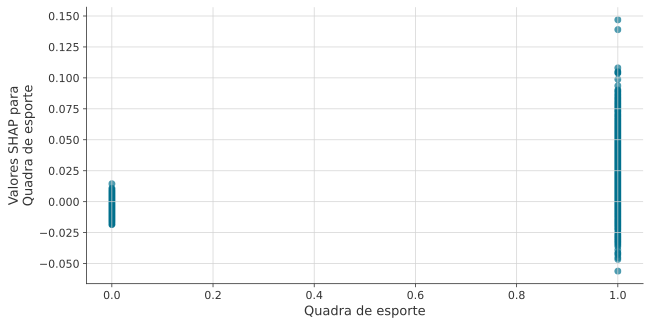
\includegraphics[keepaspectratio]{TCC_files/mediabag/includes/dependence_plot_cat/dep_plot_quadra_de_esporte2.pdf}}\end{minipage}%
%
\begin{minipage}{0.33\linewidth}
\pandocbounded{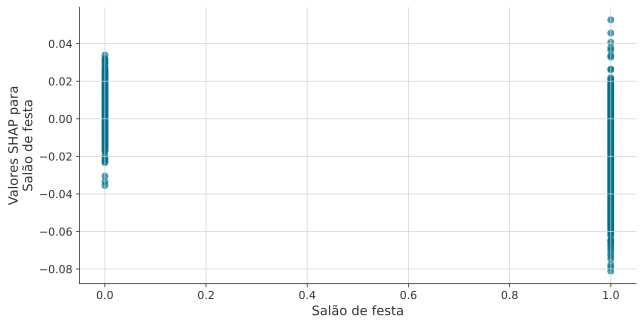
\includegraphics[keepaspectratio]{TCC_files/mediabag/includes/dependence_plot_cat/dep_plot_salao_de_festa2.pdf}}\end{minipage}%
\newline
\begin{minipage}{0.33\linewidth}
\pandocbounded{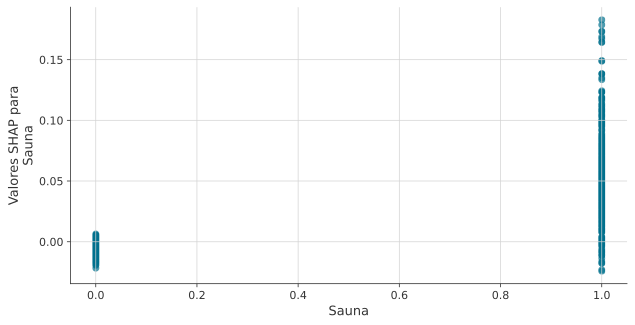
\includegraphics[keepaspectratio]{TCC_files/mediabag/includes/dependence_plot_cat/dep_plot_sauna2.pdf}}\end{minipage}%
%
\begin{minipage}{0.33\linewidth}
\pandocbounded{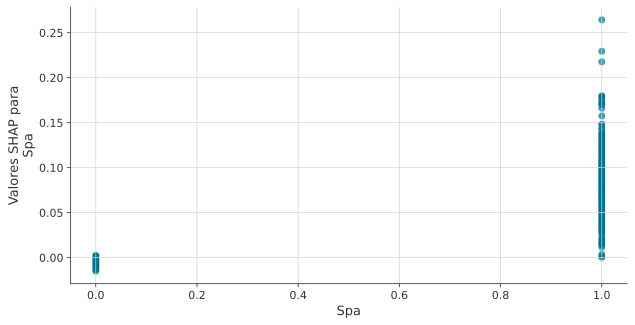
\includegraphics[keepaspectratio]{TCC_files/mediabag/includes/dependence_plot_cat/dep_plot_spa2.pdf}}\end{minipage}%
%
\begin{minipage}{0.33\linewidth}
\pandocbounded{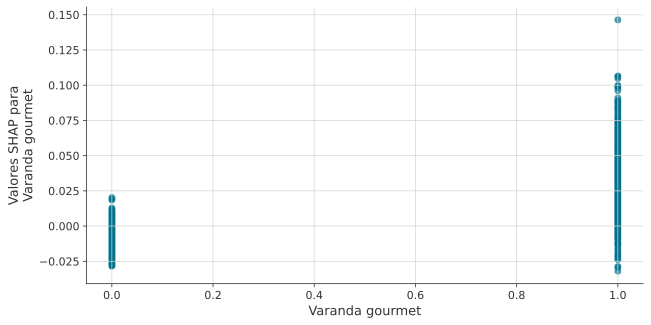
\includegraphics[keepaspectratio]{TCC_files/mediabag/includes/dependence_plot_cat/dep_plot_varanda_gourmet2.pdf}}\end{minipage}%

\caption{\label{fig-dependence_plot}Gráfico de dependência de valores
SHAP para variáveis binárias.}

\end{figure}%

\vspace{12pt}

Para a análise das variáveis binárias, foram utilizados gráficos de
dependência específicos para cada uma delas, os quais podem ser
visualizados na Figura~\ref{fig-dependence_plot}. Ao observar os valores
SHAP para imóveis com e sem academia, nota-se que a presença dessa
característica tende a elevar a predição do valor do imóvel. Um padrão
semelhante é identificado para imóveis com elevador. No entanto, mesmo
imóveis sem elevador também apresentam uma tendência de aumento na
predição, o que pode ser atribuído à interação com outras
características relevantes do imóvel.

\vspace{12pt}

Conforme já discutido na análise da importância das variáveis, sauna e
spa apresentam baixa relevância no impacto da predição do modelo. Ainda
assim, seus gráficos de dependência revelam que essas variáveis podem
contribuir para aumentar as predições em casos específicos,
especialmente em imóveis de maior valor que apresentam essas
características. O mesmo comportamento é observado para as variáveis
varanda gourmet, playground e espaço gourmet, indicando que, embora
menos relevantes no modelo de forma geral, essas características podem
ser úteis na valorização de determinados imóveis.

\begin{figure}[H]

{\centering \pandocbounded{\includegraphics[keepaspectratio]{TCC_files/mediabag/includes/lime_plot.pdf}}

}

\caption{Contribuições a partir do método LIME.}

\end{figure}%

Na figura acima, são apresentados os valores das contribuições
calculadas pelo método LIME para cada variável. Observa-se no gráfico um
padrão bastante semelhante ao identificado anteriormente pelos métodos
ICE e PDP, com a diferença de que, agora, cada cor representa um tipo
distinto de imóvel.

\vspace{12pt}

No caso da variável área, é possível observar que ela influencia
principalmente os imóveis do tipo terreno, apresentando um padrão
consistente de aumentar a predição do modelo. Isso se deve ao fato de
que terrenos, em geral, possuem áreas maiores, o que é interpretado como
um fator de valorização pelo modelo.

\vspace{12pt}

Em relação aos atributos dos imóveis, observa-se que eles têm maior
influência nas predições de apartamentos e casas. Por outro lado, a
localização se mostra um fator mais determinante para o aumento da
predição do modelo no caso de flats e terrenos, possivelmente devido à
sua maior concentração em áreas próximas à região litorânea de João
Pessoa.

\vspace{12pt}

Na seção a seguir, serão apresentados os resultados da aplicação final
desenvolvida a partir dos dados coletados por meio da abordagem de web
scraping, bem como o funcionamento prático do modelo final, o Gradient
Boosting, utilizado para a avaliação de imóveis com base em determinadas
características.

\section{Aplicação web}\label{aplicauxe7uxe3o-web}

~~~A aplicação final foi desenvolvida com o objetivo de ser simples e
intuitiva, facilitando a análise e compreensão do comportamento do
mercado imobiliário de João Pessoa. Nesta seção, serão apresentados os
resultados da aplicação e suas funcionalidades. O código completo pode
ser acessado através do seguinte link:
\url{https://github.com/cowvin0/tcc_realestate/tree/main/app}.

\vspace{12pt}

A aplicação conta com uma página principal onde o usuário pode
visualizar informações referentes aos imóveis coletados por meio do web
scraping da cidade de João Pessoa. Nessa página, são apresentados quatro
elementos gráficos. O primeiro é um gráfico de barras que exibe o valor
médio dos imóveis por bairro. O segundo, também em barras, mostra o
valor médio por tipo de imóvel. O terceiro é um histograma que
representa a distribuição dos valores individuais dos imóveis,
segmentados por tipo. Por fim, há um bloco com um mapa interativo da
cidade de João Pessoa. Por padrão, é exibido um mapa de calor com a
concentração de preços, mas o usuário pode alternar entre diferentes
tipos de visualizações geográficas com informações detalhadas da cidade.
A página inicial pode ser visualizada na Figura~\ref{fig-app}.

\begin{figure}

\centering{

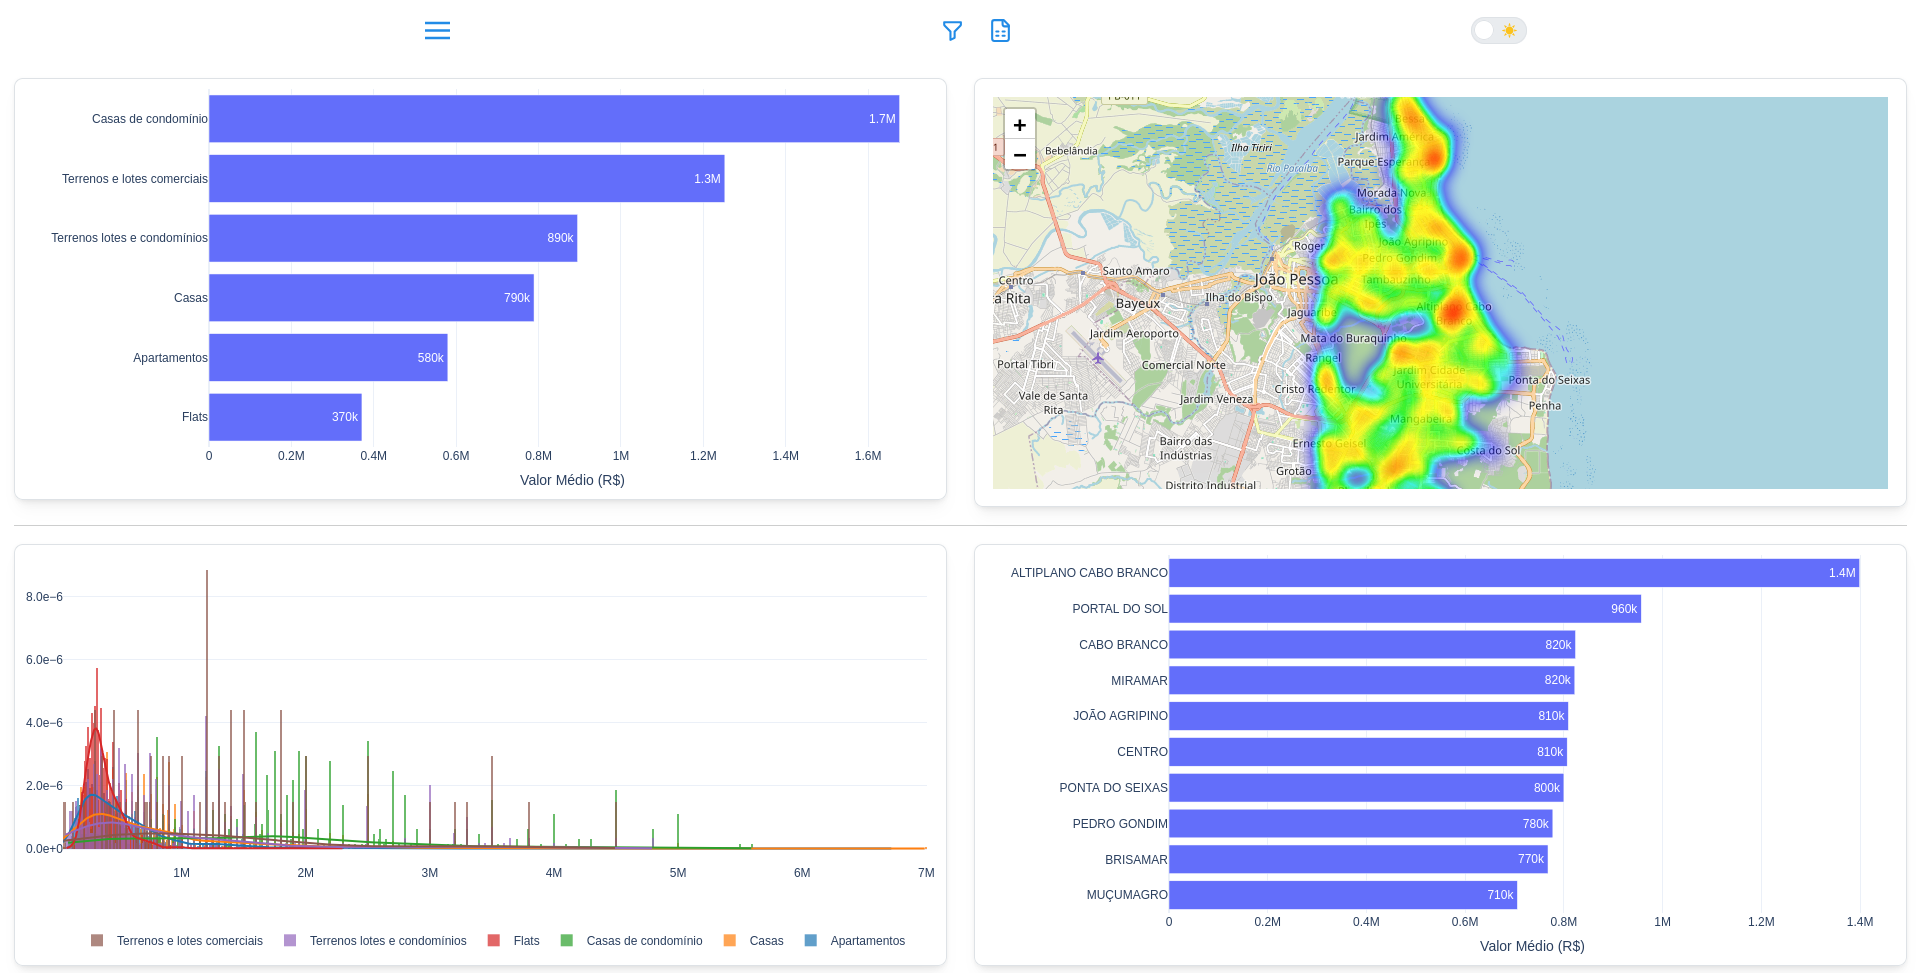
\includegraphics[width=4.6875in,height=2.60417in]{includes/screen_app.png}

}

\caption{\label{fig-app}Página da aplicação com gráfico de barras do
valor médio por tipo de imóvel, mapa de calor, histograma dos valores
dos imóveis e gráfico do valor médio por bairro.}

\end{figure}%

Com os gráficos, além de obter uma visão descritiva e analisar o
comportamento dos valores dos imóveis por bairro, o objetivo é também
permitir a aplicação de filtros. É possível filtrar os imóveis por faixa
de valor, bairros de interesse, tipos de imóvel e até mesmo por
intervalos definidos a partir da distribuição exibida no gráfico de
histograma.

\vspace{12pt}

Além dos gráficos, a aplicação oferece uma análise mais detalhada das
características dos imóveis por meio de uma tabela, apresentada na
Figura~\ref{fig-table_app}. Na figura, um retângulo vermelho destaca o
ícone de uma planilha, que pode ser clicado para exibir a visualização
da tabela. Abaixo dela, há um botão que permite o download dos dados em
formato \texttt{.csv}.

\vspace{12pt}

Essa tabela reúne todas as variáveis utilizadas no modelo, além de
incluir algumas variáveis que não foram incorporadas à modelagem, como o
IPTU e o valor do condomínio, inicialmente excluídas da base de dados
devido à alta proporção de valores ausentes.

\begin{figure}

\centering{

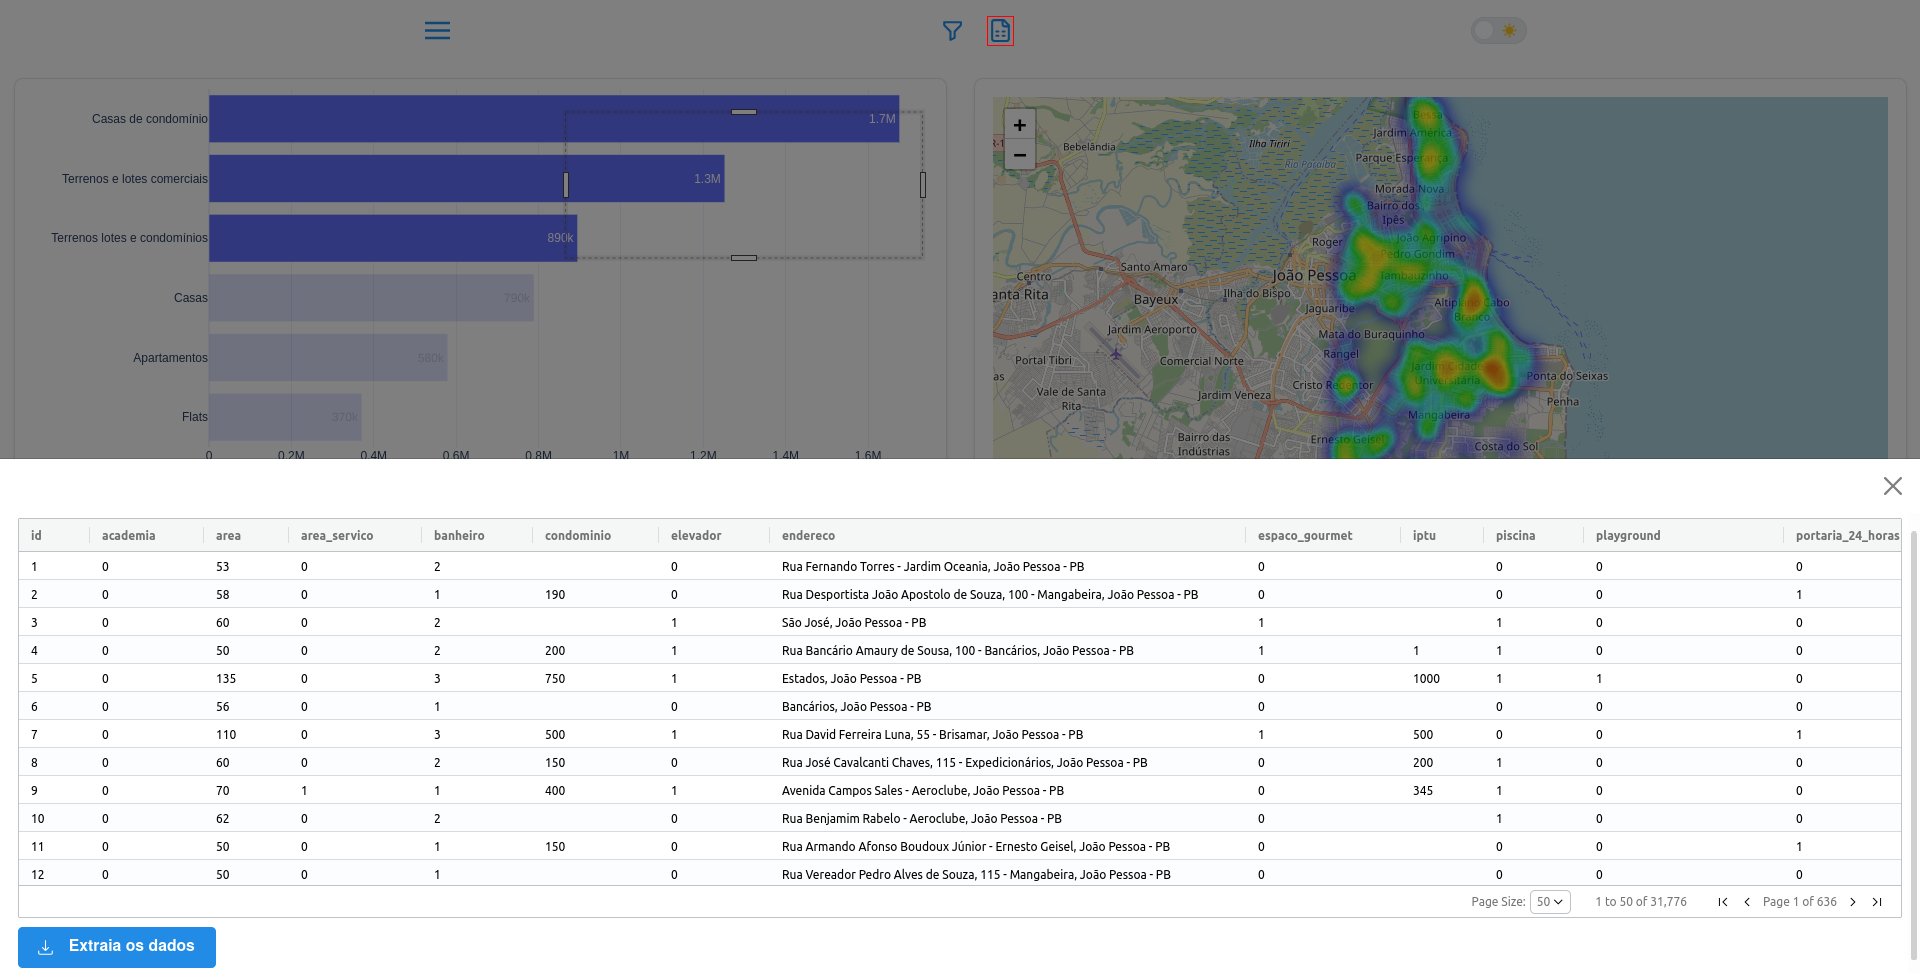
\includegraphics[width=4.6875in,height=2.60417in]{includes/table-app.png}

}

\caption{\label{fig-table_app}Tabela dos dados utilizados para predição
dos valores de imóveis.}

\end{figure}%

A funcionalidade mais importante da aplicação pode ser acessada através
do botão à direita do ícone da planilha, representado por um funil. Ao
clicar nesse botão, um menu será exibido (Figura~\ref{fig-menu_map}),
permitindo configurar o mapa e realizar previsões com o modelo final, o
Gradient Boosting.

\vspace{12pt}

Na seção de configurações do mapa, o usuário pode selecionar o tipo de
mapa desejado a partir de uma lista suspensa, que inclui todas as opções
suportadas pela aplicação. Por padrão, o mapa de calor é selecionado.
Uma das alternativas disponíveis é o mapa de pontos, que exibe a
localização dos imóveis pontualmente, com suas cores variando conforme o
valor dos imóveis, quanto mais clara a cor, mais alto o valor do imóvel.
Além desses dois mapas, a aplicação permite a visualização de
informações adicionais, como rios, ciclovias, bairros, corredores de
ônibus, faixas exclusivas para ônibus, parques, praças, área rural,
comunidades e escolas públicas.

\begin{figure}

\centering{

\includegraphics[width=4.6875in,height=2.60417in]{includes/menu_map.png}

}

\caption{\label{fig-menu_map}Controles para tipos de mapas.}

\end{figure}%

Abaixo da lista que contem os tipos de mapas, está o botão para realizar
as previsões com base nas características do imóvel passadas pelo
usuário. Ao clicar nesse botão, aparecerão diversos blocos para
preenchimento das informações do imóvel. Com as informações preenchidas,
basta utilizar o botão abaixo de todos os blocos para realizar a
estimação do valor do imóvel.

\vspace{12pt}

O usuário deve, obrigatoriamente, informar o tipo de imóvel para
realizar a predição; caso contrário, a funcionalidade não será ativada.
Após essa seleção, o usuário pode preencher as informações do imóvel.
Algumas dessas informações precisam ser selecionadas diretamente no
mapa, como as coordenadas geográficas, o valor médio do imóvel e a área
média por bairro.

\vspace{12pt}

Quando o botão para acessar as informações do imóvel é pressionado, o
mapa é automaticamente atualizado, removendo qualquer tipo previamente
selecionado e exibindo apenas o mapa vazio. Com esse mapa vazio, o
usuário deve clicar em uma localidade específica para coletar as
informações necessárias, como mostrado na
Figura~\ref{fig-map_get_coord}.

\begin{figure}

\begin{minipage}{0.50\linewidth}

\centering{

\pandocbounded{\includegraphics[keepaspectratio]{includes/map_pred.png}}

}

\subcaption{\label{fig-map_pred}}

\end{minipage}%
%
\begin{minipage}{0.50\linewidth}

\centering{

\pandocbounded{\includegraphics[keepaspectratio]{includes/map_get_coord.png}}

}

\subcaption{\label{fig-map_get_coord}}

\end{minipage}%

\caption{\label{fig-map_pred_coord}A Figura~\ref{fig-map_pred} exibe o
menu com os blocos para preenchimento das informações de imóveis,
enquanto a Figura~\ref{fig-map_get_coord} demonstra as informações
coletadas ao clicar no bairro de Altiplano.}

\end{figure}%

Embora o usuário tenha a opção de selecionar as coordenadas e as
informações de aluguel diretamente no mapa, também é possível inserir
esses dados manualmente em seus respectivos blocos de informação. Além
disso, como o KNN foi utilizado inicialmente como método de imputação
para valores ausentes, o usuário não é obrigado a fornecer todos os
dados, exceto o tipo de imóvel. Dessa forma, mesmo que algumas
informações do imóvel estejam faltando, é possível realizar a predição.
Basta deixar um ou mais campos em branco, permitindo que o KNN estime as
informações ausentes com base nas demais informações fornecidas.

\chapter{Conclusão}\label{conclusuxe3o}

~~~Neste trabalho, foi possível aplicar uma abordagem pouco usual para a
solução de problemas relacionados à avaliação do preço de imóveis,
principalmente pela dificuldade para se obter dados sobre imóveis, na
cidade de João Pessoa. A partir da utilização de técnicas de web
scraping, foi possível coletar uma base de dados abrangente diretamente
de sites de anúncios imobiliários. Esse processo automatizado de
extração de dados demonstrou-se fundamental, especialmente em contextos
onde não há acesso a bases públicas organizadas, permitindo a construção
de um conjunto rico de variáveis relevantes para a modelagem dos preços
dos imóveis.

\vspace{12pt}

Com os dados devidamente tratados e organizados, foi aplicada uma
abordagem de aprendizado de máquina, utilizando-se diferentes
algoritmos, sendo o Gradient Boosting aquele que apresentou o melhor
desempenho preditivo. O modelo final apresentou um RMSE de 227677,44,
MAPE de \(18,21\%\) e \(R^2\) de \(85,42\%\). Ou seja, obteve-se um
modelo que consegue explicar \(85,42\%\) da variância da variável
dependente e os valores estimados estão, em média, \(18,21\%\) distantes
de seus valores observados.

\vspace{12pt}

Além da modelagem, foi dada ênfase à interpretação do modelo por meio de
técnicas como SHAP, LIME, ICE e PDP. A partir dos gráficos ICE
combinados com a linha média do PDP, foi possível confirmar que imóveis
localizados mais próximos às regiões litorâneas tendem a ter valores de
predição mais elevados. O mesmo padrão de aumento nas predições foi
observado para variáveis como área do imóvel, quartos, banheiros, vagas
de garagem, quantidade de cômodos e valor do aluguel. Ou seja, à medida
que essas variáveis aumentam, maior o valor estimado pelo modelo. Por
outro lado, a variável área de aluguel apresentou um comportamento com
variações pouco expressivas nas predições, indicando um impacto mais
limitado na resposta do modelo.

\vspace{12pt}

Pelo método SHAP, observou-se que a área do imóvel foi a variável com
maior impacto na predição do modelo, sendo responsável por alterar, em
média, mais de 12\% na predição absoluta das previsões. Outras variáveis
de maior impacto nas predições foram a razão entre o número de quartos e
a área, as coordenadas geográficas e o produto entre essas coordenadas e
o valor do aluguel. Por outro lado, variáveis como sauna, spa, portaria
24 horas e quadra de esportes apresentaram menor impacto nas predições.
No entanto, os gráficos de dependência dos valores SHAP revelaram que,
embora tenham menor influência, variáveis como sauna e spa ainda são
relevantes na predição de imóveis de alto padrão, evidenciando sua
importância em casos específicos envolvendo imóveis de categorias mais
elevadas.

\vspace{12pt}

A aplicação do método LIME revelou que os atributos dos imóveis exercem
maior influência nas predições de apartamentos e casas. Em
contrapartida, a localização mostrou-se um fator mais determinante para
o aumento das predições no caso de flats e terrenos, possivelmente
devido à maior concentração desses imóveis em áreas próximas à região
litorânea. Observou-se ainda que a variável área tem impacto
especialmente relevante para os imóveis do tipo terreno, apresentando um
padrão consistente de elevação nas predições do modelo.

\vspace{12pt}

Por fim, com todos os dados coletados e o modelo final obtido, os
resultados foram integrados em uma aplicação interativa desenvolvida com
foco na análise do comportamento do mercado imobiliário de João Pessoa e
na avaliação de imóveis. A aplicação permite a visualização de mapas,
gráficos descritivos e a realização de previsões com base nas
características informadas pelo usuário. Essa ferramenta apresenta uma
abordagem ainda pouco comum na avaliação de imóveis, ao adotar métodos
mais computacionais, automatizados e orientados por dados, contribuindo
para enfrentar um dos principais desafios do setor imobiliário, que é a
escassez de informações disponíveis.

\section{Sugestões para trabalhos
futuros}\label{sugestuxf5es-para-trabalhos-futuros}

~~~Para trabalhos futuros, recomenda-se uma exploração mais aprofundada
de métodos interpretativos de modelos, como LIME, SHAP, ICE e PDP, com o
objetivo de identificar os fatores mais relevantes para a predição dos
diferentes tipos de imóveis. Essa abordagem poderia, inclusive,
contribuir para melhorar as predições em observações nas quais o modelo
apresenta maior erro.

\vspace{12pt}

Também é sugerido uma investigação mais detalhada sobre o ajuste do
modelo, a fim de avaliar sua capacidade de generalização. Além disso,
sugere-se analisar o impacto da tunagem de hiperparâmetros no desempenho
preditivo dos modelos e na comparação entre eles. Outra possibilidade
interessante seria explorar metodologias alternativas para a predição
dos valores dos imóveis, como, por exemplo, o uso de Redes Neurais.

\chapter*{\texorpdfstring{\centering Referências}{Referências}}\label{referuxeancias}

\markboth{Referências}{Referências}

\phantomsection\label{refs}
\begin{CSLReferences}{0}{1}
\bibitem[\citeproctext]{ref-abecip_credito2007}
ABECIP. \textbf{O Crédito Imobiliário no Brasil: Caracterização e
Desafios}. {[}S.l.{]}: Associação Brasileira das Entidades de Crédito
Imobiliário e Poupança, 2007b.

\bibitem[\citeproctext]{ref-revolucao_credito_imobiliario}
\_\_\_\_\_\_. \textbf{A Revolução do Crédito Imobiliário: 44 Anos
(1967--2011)}. {[}S.l.{]}: Associação Brasileira das Entidades de
Crédito Imobiliário e Poupança, 2007a.

\bibitem[\citeproctext]{ref-abecip_monografia}
\_\_\_\_\_\_. \textbf{IV Prêmio ABECIP de Monografia em Crédito
Imobiliário e Poupança}. {[}S.l.{]}: Associação Brasileira das Entidades
de Crédito Imobiliário e Poupança, 2015.

\bibitem[\citeproctext]{ref-optuna_2019}
AKIBA, T. et al. Optuna: A Next-generation Hyperparameter Optimization
Framework. {[}S.l.{]}: {[}s.n.{]}, 2019.

\bibitem[\citeproctext]{ref-quarto}
ALLAIRE, J.; DERVIEUX, C.
\textbf{\href{https://CRAN.R-project.org/package=quarto}{quarto: R
Interface to 'Quarto' Markdown Publishing System}}. {[}S.l.{]}:
{[}s.n.{]}, 2024.

\bibitem[\citeproctext]{ref-assumpccao2011credito}
ASSUMPÇÃO FILHO, C. A. B. O cr{é}dito imobili{á}rio no Brasil. 2011.

\bibitem[\citeproctext]{ref-sqlalchemy}
BAYER, M. \href{http://aosabook.org/en/sqlalchemy.html}{SQLAlchemy}.
\emph{Em}: BROWN, A.; WILSON, G. (Org.). \textbf{The Architecture of
Open Source Applications Volume II: Structure, Scale, and a Few More
Fearless Hacks}. {[}S.l.{]}: aosabook.org, 2012.

\bibitem[\citeproctext]{ref-bergstra2011algorithms}
BERGSTRA, J. et al. Algorithms for hyper-parameter optimization.
\textbf{Advances in neural information processing systems}, 2011. v. 24.

\bibitem[\citeproctext]{ref-bergstra2013making}
\_\_\_\_\_\_; YAMINS, D.; COX, D. Making a science of model search:
Hyperparameter optimization in hundreds of dimensions for vision
architectures. {[}S.l.{]}: PMLR, 2013. p. 115--123.

\bibitem[\citeproctext]{ref-bischl2023hyperparameter}
BISCHL, B. et al. Hyperparameter optimization: Foundations, algorithms,
best practices, and open challenges. \textbf{Wiley Interdisciplinary
Reviews: Data Mining and Knowledge Discovery}, 2023. v. 13, n. 2, p.
e1484.

\bibitem[\citeproctext]{ref-breiman1996bagging}
BREIMAN, L. Bagging predictors. \textbf{Machine learning}, 1996. v. 24,
p. 123--140.

\bibitem[\citeproctext]{ref-geocoder}
CAMBON, J. et al. tidygeocoder: An R package for geocoding.
\textbf{Journal of Open Source Software}, 2021. v. 6, n. 65, p. 3544.
Disponível em:
\textless{}\url{https://doi.org/10.21105/joss.03544}\textgreater.

\bibitem[\citeproctext]{ref-campos2014precificaccao}
CAMPOS, S. F. Precifica{ç}{ã}o de im{ó}veis e seus elementos agregadores
de valor sob a vis{ã}o do consumidor: uma an{á}lise do mercado
imobili{á}rio de Jo{ã}o Pessoa-PB. 2014.

\bibitem[\citeproctext]{ref-chen2016xgboost}
CHEN, T.; GUESTRIN, C. Xgboost: A scalable tree boosting system.
{[}S.l.{]}: {[}s.n.{]}, 2016. p. 785--794.

\bibitem[\citeproctext]{ref-cohen2009pearson}
COHEN, I. et al. Pearson correlation coefficient. \textbf{Noise
reduction in speech processing}, 2009. p. 1--4.

\bibitem[\citeproctext]{ref-evolucao_abecip}
COSTA FARIAS, B. M. Da. A evolu{ç}{ã}o do mercado imobili{á}rio
brasileiro e o conceito de Home Equity. 2010.

\bibitem[\citeproctext]{ref-fipe_metodologia}
FIPE -- FUNDAÇÃO INSTITUTO DE PESQUISAS ECONÔMICAS. \textbf{Índice
FipeZap de Preços de Imóveis Anunciados: Notas Metodológicas}. São
Paulo: Fipe, 2024.

\bibitem[\citeproctext]{ref-friedman2002stochastic}
FRIEDMAN, J. H. Stochastic gradient boosting. \textbf{Computational
statistics \& data analysis}, 2002. v. 38, n. 4, p. 367--378.

\bibitem[\citeproctext]{ref-garnett2023bayesian}
GARNETT, R. \textbf{Bayesian optimization}. {[}S.l.{]}: Cambridge
University Press, 2023.

\bibitem[\citeproctext]{ref-goldstein2015peeking}
GOLDSTEIN, A. et al. Peeking inside the black box: Visualizing
statistical learning with plots of individual conditional expectation.
\textbf{journal of Computational and Graphical Statistics}, 2015. v. 24,
n. 1, p. 44--65.

\bibitem[\citeproctext]{ref-harris2020array}
HARRIS, C. R. et al. Array programming with {NumPy}. \textbf{Nature},
set. 2020. v. 585, n. 7825, p. 357--362. Disponível em:
\textless{}\url{https://doi.org/10.1038/s41586-020-2649-2}\textgreater.

\bibitem[\citeproctext]{ref-hastie2009elements}
HASTIE, T. et al. \textbf{The elements of statistical learning: data
mining, inference, and prediction}. {[}S.l.{]}: Springer, 2009. V. 2.

\bibitem[\citeproctext]{ref-holston1989modernist}
HOLSTON, J. \textbf{The modernist city: An anthropological critique of
Brasilia}. {[}S.l.{]}: University of Chicago Press, 1989.

\bibitem[\citeproctext]{ref-shammamah_hossain-proc-scipy-2019}
HOSSAIN, Shammamah.
\href{https://doi.org/10.25080/Majora-7ddc1dd1-012}{{V}isualization of
{B}ioinformatics {D}ata with {D}ash {B}io}. (Chris Calloway et al.,
Org.). {[}S.l.{]}: {[}s.n.{]}, 2019. p. 126--133.

\bibitem[\citeproctext]{ref-Hunter:2007}
HUNTER, J. D. \href{https://doi.org/10.1109/MCSE.2007.55}{Matplotlib: A
2D graphics environment}. \textbf{Computing in Science \& Engineering},
2007. v. 9, n. 3, p. 90--95.

\bibitem[\citeproctext]{ref-pmlr-v32-hutter14}
HUTTER, F.; HOOS, H.; LEYTON-BROWN, K. An Efficient Approach for
Assessing Hyperparameter Importance. (E. P. Xing \& T. Jebara, Org.).
Bejing, China: PMLR, 2014. V. 32, p. 754--762. Disponível em:
\textless{}\url{https://proceedings.mlr.press/v32/hutter14.html}\textgreater.

\bibitem[\citeproctext]{ref-plotly}
INC., P. T. Collaborative data science. 2015. Disponível em:
\textless{}\url{https://plot.ly}\textgreater.

\bibitem[\citeproctext]{ref-izbicki2020aprendizado}
IZBICKI, R.; SANTOS, T. M. Dos. \textbf{Aprendizado de m{á}quina: uma
abordagem estat{ı́}stica}. {[}S.l.{]}: Rafael Izbicki, 2020.

\bibitem[\citeproctext]{ref-james2013introduction}
JAMES, G. et al. \textbf{An introduction to statistical learning}.
{[}S.l.{]}: Springer, 2013. V. 112.

\bibitem[\citeproctext]{ref-ke2017lightgbm}
KE, G. et al. Lightgbm: A highly efficient gradient boosting decision
tree. \textbf{Advances in neural information processing systems}, 2017.
v. 30.

\bibitem[\citeproctext]{ref-kouzis2016learning}
KOUZIS-LOUKAS, D. \textbf{Learning Scrapy}. {[}S.l.{]}: Packt Publishing
Ltd, 2016.

\bibitem[\citeproctext]{ref-NIPS2017_7062}
LUNDBERG, S. M.; LEE, S.-I.
\href{http://papers.nips.cc/paper/7062-a-unified-approach-to-interpreting-model-predictions.pdf}{A
Unified Approach to Interpreting Model Predictions}. \emph{Em}: GUYON,
I. et al. (Org.). \textbf{Advances in Neural Information Processing
Systems 30}. {[}S.l.{]}: Curran Associates, Inc., 2017, p. 4765--4774.

\bibitem[\citeproctext]{ref-molnar2020interpretable}
MOLNAR, C. \textbf{Interpretable machine learning}. {[}S.l.{]}: Lulu.
com, 2020.

\bibitem[\citeproctext]{ref-scikit-learn}
PEDREGOSA, F. et al. Scikit-learn: Machine Learning in {P}ython.
\textbf{Journal of Machine Learning Research}, 2011. v. 12, p.
2825--2830.

\bibitem[\citeproctext]{ref-folium}
PYTHON-VISUALIZATION. \textbf{Folium}. Disponível em:
\textless{}\url{https://python-visualization.github.io/folium/}\textgreater.

\bibitem[\citeproctext]{ref-r_language}
R CORE TEAM. \textbf{\href{https://www.R-project.org/}{R: A Language and
Environment for Statistical Computing}}. Vienna, Austria: R Foundation
for Statistical Computing, 2024.

\bibitem[\citeproctext]{ref-ribeiro2016should}
RIBEIRO, M. T.; SINGH, S.; GUESTRIN, C. " Why should i trust you?"
Explaining the predictions of any classifier. {[}S.l.{]}: {[}s.n.{]},
2016. p. 1135--1144.

\bibitem[\citeproctext]{ref-shapley1953value}
SHAPLEY, L. S. A value for n-person games. \textbf{Contribution to the
Theory of Games}, 1953. v. 2.

\bibitem[\citeproctext]{ref-snoek2012practical}
SNOEK, J.; LAROCHELLE, H.; ADAMS, R. P. Practical bayesian optimization
of machine learning algorithms. \textbf{Advances in neural information
processing systems}, 2012. v. 25.

\bibitem[\citeproctext]{ref-spearman1961proof}
SPEARMAN, C. The proof and measurement of association between two
things. 1961.

\bibitem[\citeproctext]{ref-vstrumbelj2014explaining}
ŠTRUMBELJ, E.; KONONENKO, I. Explaining prediction models and individual
predictions with feature contributions. \textbf{Knowledge and
information systems}, 2014. v. 41, p. 647--665.

\bibitem[\citeproctext]{ref-reback2020pandas}
TEAM, T. Pandas Development. \textbf{pandas-dev/pandas: Pandas}. Zenodo.
Disponível em:
\textless{}\url{https://doi.org/10.5281/zenodo.3509134}\textgreater.

\bibitem[\citeproctext]{ref-selenium}
THORPE, A.
\textbf{\href{https://CRAN.R-project.org/package=selenium}{selenium:
Low-Level Browser Automation Interface}}. {[}S.l.{]}: {[}s.n.{]}, 2024.

\bibitem[\citeproctext]{ref-van1995python}
VAN ROSSUM, G.; DRAKE JR, F. L. \textbf{Python reference manual}.
{[}S.l.{]}: Centrum voor Wiskunde en Informatica Amsterdam, 1995.

\bibitem[\citeproctext]{ref-2020SciPy-NMeth}
VIRTANEN, P. et al.
\href{https://doi.org/10.1038/s41592-019-0686-2}{{{SciPy} 1.0:
Fundamental Algorithms for Scientific Computing in Python}}.
\textbf{Nature Methods}, 2020. v. 17, p. 261--272.

\bibitem[\citeproctext]{ref-wagner1980urbanization}
WAGNER, F. E.; WARD, J. O. Urbanization and Migration in Brazil.
\textbf{The American Journal of Economics and Sociology}, 1980. v. 39,
n. 3, p. 249--259.

\bibitem[\citeproctext]{ref-Waskom2021}
WASKOM, M. L. seaborn: statistical data visualization. \textbf{Journal
of Open Source Software}, 2021. v. 6, n. 60, p. 3021. Disponível em:
\textless{}\url{https://doi.org/10.21105/joss.03021}\textgreater.

\bibitem[\citeproctext]{ref-httr}
WICKHAM, H. \textbf{\href{https://CRAN.R-project.org/package=httr}{httr:
Tools for Working with URLs and HTTP}}. {[}S.l.{]}: {[}s.n.{]}, 2023.

\bibitem[\citeproctext]{ref-rvest}
\_\_\_\_\_\_. \textbf{\href{https://rvest.tidyverse.org/}{rvest: Easily
Harvest (Scrape) Web Pages}}. {[}S.l.{]}: {[}s.n.{]}, 2024.

\bibitem[\citeproctext]{ref-xml2}
\_\_\_\_\_\_; HESTER, J.; OOMS, J.
\textbf{\href{https://xml2.r-lib.org/}{xml2: Parse XML}}. {[}S.l.{]}:
{[}s.n.{]}, 2023.

\bibitem[\citeproctext]{ref-yang2020hyperparameter}
YANG, L.; SHAMI, A. On hyperparameter optimization of machine learning
algorithms: Theory and practice. \textbf{Neurocomputing}, 2020. v. 415,
p. 295--316.

\bibitem[\citeproctext]{ref-yeo}
YEO, I.-K.; JOHNSON, R. A. A New Family of Power Transformations to
Improve Normality or Symmetry. \textbf{Biometrika}, 2000. v. 87, n. 4,
p. 954--959. Disponível em:
\textless{}\url{http://www.jstor.org/stable/2673623}\textgreater. Acesso
em: 25 out. 2023.

\end{CSLReferences}




\end{document}
